
\chapter{Multiple Integrals}

\section*{Introduction}

In single-variable calculus, integration lets us accumulate a quantity along a line segment---the area under a curve, the total distance traveled, the mass of a wire. But the real world is two- and three-dimensional: how much rain fell on a field? What is the mass of a planet with varying density? How much heat flows through a curved surface? To answer questions like these, we need to integrate over flat regions, curved surfaces, and solid bodies. That is what multiple integrals do.\\ \\
\noindent The core idea is not as intimidating as it sounds---we are just adding up small pieces, exactly as before, but now in higher dimensions. A double integral sums over a region in the plane; a triple integral sums over a solid in space. The mechanics are an extension of single-variable integration: we evaluate iterated integrals by integrating one variable at a time, peeling away dimensions layer by layer.\\ \\
\noindent What makes this chapter genuinely powerful is the interplay between geometry and coordinate systems. Many integrals that are nightmarish in Cartesian coordinates become routine in polar, cylindrical, or spherical coordinates---the right choice of coordinates can turn pages of algebra into a few clean lines. We formalize this idea through the \textbf{Jacobian determinant}, which tells us exactly how area and volume elements transform when we switch coordinate systems. This machinery unifies every coordinate change we perform, from the familiar \( r\,dr\,d\theta \) of polar coordinates to exotic transformations tailored to specific geometries.\\ \\
\noindent Along the way, we apply multiple integrals to compute areas, volumes, surface areas, centers of mass, moments of inertia, and average values---the workhorses of physics and engineering. By the end of this chapter, you will be able to set up and evaluate integrals over virtually any region in two or three dimensions.


\newpage 





\lecture{Double Integrals over Rectangular Regions} \index{Double Integrals} \index{Rectangular Regions}

\noindent In our study of single-variable calculus, we encountered the definite integral as a powerful tool for computing accumulated change. Given a function \(f(x)\), we interpreted \(\int_a^b f(x)\,dx\) as the signed area between the curve and the $x$-axis—a measurement of how a quantity accumulates along a one-dimensional interval. But what happens when we want to measure accumulation over a two-dimensional region? \\ \\
Consider, for instance, the temperature distribution across a metal plate, the density variation in a thin sheet of material, or the pressure distribution across a surface. These scenarios involve quantities that vary with both $x$ and $y$ coordinates. How might we extend our understanding of integration to capture such two-dimensional variation? \\ \\
Just as we built the single integral from the concept of adding up infinitesimally thin rectangles, we can imagine building a two-dimensional integral by adding up infinitesimally small rectangular pieces of a surface. This generalization leads us to the concept of a double integral—a fundamental tool for analyzing change across two-dimensional regions.

\begin{figure}[H]
\centering
\tdplotsetmaincoords{70}{110}
\begin{tikzpicture}[tdplot_main_coords,line cap=round,>=stealth,
    declare function={f(\x,\y)=3+0.5*sin(30*\x)*cos(30*\y);}]
 \draw[->] (0,0,0) coordinate (O) -- (5,0,0) node[pos=1.05]{$x$};
 \draw[->] (O) -- (0,5,0) node[pos=1.05]{$y$};
 \draw[->] (O) -- (0,0,5) node[pos=1.05]{$z$};
 \draw (1,2,0) -- (2,2,0)   -- (2,3,0) -- (1,3,0) -- cycle;
 \foreach \X in {1,2} {\foreach \Y in {2,3} 
   {\draw[dashed] (\X,\Y,0) -- (\X,\Y,{f(\X,\Y)});}}    
 \foreach \X in {1,2} {
   \draw[dashed] (\X,2,0) -- (\X,0,0);}
 \foreach \Y in {2,3} {
   \draw[dashed] (1,\Y,0) -- (0,\Y,0);}
 \foreach \X in {0,...,4}
  {\draw plot[variable=\x,domain=0:5,smooth] (\X,\x,{f(\X,\x)});
   }
 \foreach \Y in {0,...,5}
  {\draw plot[variable=\x,domain=0:4,smooth] (\x,\Y,{f(\x,\Y)});
   }
 \draw[blue,thick] plot[variable=\x,domain=1:2]  (\x,2,{f(\x,2)})
    -- plot[variable=\y,domain=2:3]  (2,\y,{f(2,\y)})
    -- plot[variable=\x,domain=2:1]  (\x,3,{f(\x,3)})
    -- plot[variable=\y,domain=3:2]  (1,\y,{f(1,\y)})
    -- cycle;
\end{tikzpicture}
\caption{\textit{The integral extends naturally to higher dimensions. Above we see the volume under the surface: the multivariate analog to the area under a curve.}}
\end{figure}


\subsection*{Definition and Interpretation} \index{Double Integrals}

\noindent Let's begin with the simplest case: a continuous function \(f(x,y)\) defined over a rectangular region \(R = [a,b] \times [c,d]\) in the \(xy\)-plane. What might it mean to integrate this function over $R$? In single-variable calculus, our integrand \(f(x)\) traced out a curve above the x-axis, and we found the area beneath it. Here, our function \(f(x,y)\) traces out a surface above the $xy$-plane, suggesting that our integral should measure the volume beneath this surface. \\ \\
We denote this double integral as:
\[
\iint_R f(x,y) \, dA,
\]
where \(dA\) represents an infinitesimal element of area, just as \(dx\) represented an infinitesimal length in single-variable calculus. This notation, with its double integral sign, reflects the two-dimensional nature of our accumulation. Note that we will begin writing a set as a subscript to the integral to indicate the bounds of integration. We will begin using this more, and using either sets or product sets listed as $A,B,R,R_i$, or $[a,b],[2,5],(-\infty,4)$, or $A \times B, [a,b] \times [c,d]$ or $[-1,1]^2$ and so on. \\ \\
But what exactly are we accumulating? The value \(f(x,y)\) at each point can be thought of as a ``height" above the $xy$-plane, and when we multiply this height by a small area \(dA\), we get a small volume element. The double integral sums up all these infinitesimal volumes over the region $R$, giving us the total signed volume between the surface \(z = f(x,y)\) and the $xy$-plane. \\ \\
To make this intuition precise, we need to follow the same path that led us to the Riemann integral in single-variable calculus. How might we approximate this volume before taking a limit? Just as we divided an interval into subintervals, we can partition our rectangle $R$ into smaller rectangles and approximate the volume above each piece.

\subsubsection*{Construction via Riemann Sums} \index{Riemann Sum}

\noindent Recall how we constructed the single integral: we divided our interval into smaller pieces, chose a sample point in each piece, multiplied by the width of the piece, and took the limit as the pieces became infinitesimally small. For a double integral, we follow a similar path, but now we're working with two-dimensional pieces. \\ \\
Let's construct this systematically. First, we'll partition our rectangular region R into a grid of smaller rectangles. How do we do this? We can divide each side of our rectangle independently:
\begin{itemize}
    \item Partition \([a,b]\) into \(n\) equal subintervals, each of width \(\Delta x = \frac{b-a}{n}\)
    \item Partition \([c,d]\) into \(m\) equal subintervals, each of height \(\Delta y = \frac{d-c}{m}\)
\end{itemize}

\noindent This creates a grid of \(nm\) small rectangles, which we'll call \(R_{ij}\). Each has area \(\Delta A = \Delta x \Delta y\). Just as we chose a sample point in each subinterval for single integrals, here we choose a sample point \((x_{ij}^*, y_{ij}^*)\) in each small rectangle. \\ \\
Now we can build our approximation. Above each small rectangle \(R_{ij}\), we have an approximately rectangular solid with:
\begin{itemize}
    \item Base area: \(\Delta A = \Delta x \Delta y\)
    \item Height: \(f(x_{ij}^*, y_{ij}^*)\)
    \item Volume: \(f(x_{ij}^*, y_{ij}^*)\Delta A\)
\end{itemize}

\noindent Adding up all these small volumes gives us our double Riemann sum:
\[
S_{n,m} = \sum_{i=1}^n \sum_{j=1}^m f(x_{ij}^*, y_{ij}^*) \Delta A
\]

\noindent Just as the definite integral emerged as the limit of Riemann sums, we define the double integral as the limit of these double Riemann sums as our grid becomes infinitely fine:
\[
\iint_R f(x,y) \, dA = \lim_{n,m \to \infty} S_{n,m} = \lim_{n,m \to \infty} \sum_{i=1}^n \sum_{j=1}^m f(x_{ij}^*, y_{ij}^*) \Delta A
\]

\noindent This limit, when it exists, gives us the precise value of the double integral. For continuous functions (and even some discontinuous ones), this limit exists and is independent of how we choose our sample points \((x_{ij}^*, y_{ij}^*)\)—a remarkable fact that parallels the single-variable case. \\ \\
This construction gives us more than just a definition; it provides a concrete way to visualize what a double integral actually computes. We're literally adding up infinitely many infinitesimally small volumes, just as a single integral adds up infinitely many infinitesimally thin rectangles. The figure below is the 3D representation of the Riemann sums under a surface:

\begin{figure}[H]
\centering
\begin{tikzpicture}[y={(0:1cm)},x={(225:0.86cm)}, z={(90:1cm)}]

% coordinates for the lower grid
\path
  (1,3,0) coordinate (bm0) -- 
  (4,3,0) coordinate (fm0) coordinate[midway] (lm0) --
  (4,8,0) coordinate[pos=0.25] (fm1) coordinate[midway] (fm2) coordinate[pos=0.75] (fm3) coordinate (fm4) --
  (1,8,0) coordinate (bm4) coordinate[midway] (lm4)--
  (bm0) coordinate[pos=0.25] (bm3) coordinate[midway] (bm2) coordinate[pos=0.75] (bm1);
\draw[dashed]
  (lm0) -- 
  (lm4) coordinate[pos=0.25] (lm1) coordinate[midway] (lm2) coordinate[pos=0.75] (lm3);

% the blocks
\DrawBlock{b}{1}{4}
\DrawBlock{b}{2}{3.7}
\DrawBlock{b}{3}{4.3}
\DrawBlock{b}{4}{5}
\DrawBlock{f}{1}{3.3}
\DrawBlock{f}{2}{3.5}
\DrawBlock{f}{3}{4}
\DrawBlock{f}{4}{4.7}

\foreach \Point/\Height in {lm1/3.7,lm2/4.3,lm3/5}
  \draw[ultra thin,dashed,opacity=0.2] (\Point) -- ++(0,0,\Height);

% the lower grid
\foreach \x in {1,2,3}
  \draw[dashed] (fm\x) -- (bm\x);
\draw[dashed] (fm0) -- (bm0) -- (bm4);
\draw (fm0) -- (fm4) -- (bm4);
\draw[dashed] (lm0) -- (lm4);

% coordinates for the surface
\coordinate (curvefm0) at ( $ (fm0) + (0,0,4) $ );
\coordinate (curvebm0) at ( $ (bm0) + (0,0,4) $ );
\coordinate (curvebm4) at ( $ (bm4) + (0,0,6) $ );
\coordinate (curvefm4) at ( $ (fm4) + (0,0,5.7) $ );

% the surface
\filldraw[ultra thick,fill=gray!25,fill opacity=0.2]
  (curvefm0) to[out=-30,in=210] 
  (curvefm4) to[out=-4,in=260]
  (curvebm4) to[out=215,in=330]
  (curvebm0) to[out=240,in=-20]
  (curvefm0);

% lines from grid to surface
\draw[very thick,name path=leftline] (curvefm0) -- (fm0);
\draw[very thick] (curvefm4) -- (fm4);
\draw[very thick,name path=rightline] (curvebm4) -- (bm4);
\draw[very thick,dashed] (curvebm0) -- (bm0);

% coordinate system
\coordinate (O) at (0,0,0);
\draw[-latex] (O) -- +(5,0,0) node[above left] {$x$};
\path[name path=yaxis] (O) -- +(0,10,0) coordinate (yaxisfinal) node[above] {$y$};
\draw[-latex] (O) -- +(0,0,5) node[left] {$z$};
\path[name intersections={of=yaxis and leftline,by={yaxis1}}];
\path[name intersections={of=yaxis and rightline,by={yaxis2}}];
\draw (O) -- (yaxis1);
\draw[densely dashed,opacity=0.1] (yaxis1) -- (yaxis2);
\draw[-latex] (yaxis2) -- (yaxisfinal);

% for debugging
%\foreach \Name in {bm0,fm0,lm0,fm1,fm2,fm3,fm4,bm4,lm4,bm1,bm2,bm3,lm1,lm2,lm3,%
%curvefm0,curvebm0,curvebm4,curvefm4}
%  \node at (\Name) {\Name};  
\end{tikzpicture} 
\caption{\textit{The Riemann Sum approximation of the volume under a surface. When taking the limit of these rectangular prisms to be infinitesimally small, we approximate the double integral.}}
\end{figure}
\noindent It is important to also note, that just as we have the idea of \textbf{negative area} in single variable calculus when the curve dips below the $x$-axis, we also have the analogous \textbf{negative volume} when our surface dips below the $xy$-plane.

\exampleline
\begin{example}
Approximate the double integral \(\iint_R f(x,y)\,dA\) where \(f(x,y) = x^2 + y^2\) over the rectangular region \(R = [0,2] \times [0,1]\) using a Riemann sum with \(n = 2\) subintervals in $x$ and \(m = 2\) subintervals in $y$. Use the upper-right corner of each subrectangle as the sample point.

\begin{solution}
Let's construct this approximation systematically:

\begin{enumerate}
\item First, let's determine our partition dimensions:
    \[
    \Delta x = \frac{2-0}{2} = 1, \quad \Delta y = \frac{1-0}{2} = \frac{1}{2}
    \]
    So each subrectangle has area:
    \[
    \Delta A = \Delta x \Delta y = (1)\left(\frac{1}{2}\right) = \frac{1}{2}
    \]

\item The $x$-coordinates of our partition are:
    \[
    x_0 = 0, \quad x_1 = 1, \quad x_2 = 2
    \]
    The $y$-coordinates are:
    \[
    y_0 = 0, \quad y_1 = \frac{1}{2}, \quad y_2 = 1
    \]

\item Using upper-right corners as sample points, our four subrectangles have points:
    \begin{align*}
    R_{11}: &\quad (x_{11}^*, y_{11}^*) = \left(1, \frac{1}{2}\right) \\
    R_{12}: &\quad (x_{12}^*, y_{12}^*) = \left(1, 1\right) \\
    R_{21}: &\quad (x_{21}^*, y_{21}^*) = \left(2, \frac{1}{2}\right) \\
    R_{22}: &\quad (x_{22}^*, y_{22}^*) = \left(2, 1\right)
    \end{align*}

\item Evaluate \(f(x,y) = x^2 + y^2\) at each sample point:
    \begin{align*}
    f\left(1, \frac{1}{2}\right) &= 1 + \frac{1}{4} = \frac{5}{4} \\
    f(1, 1) &= 1 + 1 = 2 \\
    f\left(2, \frac{1}{2}\right) &= 4 + \frac{1}{4} = \frac{17}{4} \\
    f(2, 1) &= 4 + 1 = 5
    \end{align*}

\item Form the double Riemann sum:
    \begin{align*}
    S_{2,2} &= \sum_{i=1}^2 \sum_{j=1}^2 f(x_{ij}^*, y_{ij}^*) \Delta A \\
    &= \frac{1}{2}\left[f\left(1,\frac{1}{2}\right) + f(1,1) + f\left(2,\frac{1}{2}\right) + f(2,1)\right] \\
    &= \frac{1}{2}\left[\frac{5}{4} + 2 + \frac{17}{4} + 5\right] \\
    &= \frac{1}{2}\left[\frac{5 + 8 + 17 + 20}{4}\right] \\
    &= \frac{50}{8} = \frac{25}{4} = 6.25
    \end{align*}
\end{enumerate}

\noindent Therefore, our Riemann sum approximation is \(\frac{25}{4}\) or approximately 6.25 cubic units. This is a rough approximation; the actual value of the double integral would be obtained by taking the limit as \(n,m \to \infty\). \\ \\
Note: This example illustrates how even a coarse partition (2×2) involves significant computation. The true power of double integrals emerges when we develop more sophisticated techniques (like Fubini's Theorem) to evaluate them exactly rather than approximating with Riemann sums.
\end{solution}
\end{example}
\exampleline

\subsubsection*{Types of Riemann Sums} \index{Riemann Sum Types}

\noindent Just as in single-variable calculus, where we could choose different sample points in each subinterval (left endpoint, right endpoint, midpoint), we have analogous choices for double integrals. Recall from Chapter 1 Lecture 1 that we listed different approximation techniques: left-hand sums tended to overestimate decreasing functions, right-hand sums underestimated them, and midpoint sums often provided better approximations. \\ \\
For double integrals, we have similar options for choosing our sample points \((x_{ij}^*, y_{ij}^*)\) in each subrectangle \(R_{ij}\):

\begin{itemize}
   \item \textbf{Lower-Left Corner:} Take \((x_{ij}^*, y_{ij}^*)\) as the lower-left vertex of each \(R_{ij}\)
   \item \textbf{Upper-Right Corner:} Use the upper-right vertex of each \(R_{ij}\)
   \item \textbf{Center Point:} Choose the center point of each \(R_{ij}\)
   \item \textbf{Supremum/Infimum:} Select points where \(f\) achieves its maximum/minimum value in \(R_{ij}\)
\end{itemize}

\noindent Just as with single integrals, these choices can lead to over- or under-approximations. For instance, if \(f(x,y)\) is increasing in both variables, the lower-left corners will give an underestimate, while upper-right corners will give an overestimate. The center point method often provides a better approximation, as it tends to balance out these extremes. \\ \\ Importantly, for continuous functions, all these methods converge to the same limit as the mesh of our partition becomes infinitely fine. This convergence mirrors the behavior we saw with single integrals and reinforces a fundamental principle: while the choice of sample points affects our approximations, it does not affect the final value of the integral.

\subsection*{Fubini's Theorem and Iterated Integrals} \index{Fubini's Theorem}

\noindent Now that we understand what a double integral represents and how to approximate it, a natural question arises: how do we actually compute one? The Riemann sum definition, while theoretically important, isn't practical for calculation. Just as we developed techniques to evaluate single integrals without resorting to Riemann sums, we need efficient methods for double integrals. \\ \\
The key insight comes from examining how we might systematically accumulate volume. Looking at our rectangular region $R = [a,b] \times [c,d]$, we could:
\begin{itemize}
   \item First, for each fixed $x$-value, integrate along the $y$-direction to find the area of a cross-sectional slice
   \item Then, integrate these slice areas along the $x$-axis to get the total volume
\end{itemize}
This intuition leads us to one of the most powerful results in multivariable calculus: Fubini's Theorem.

\subsubsection*{Statement of Fubini's Theorem}

\noindent For a continuous function $f(x,y)$ on a rectangular region $R = [a,b] \times [c,d]$, Fubini's Theorem states that we can compute the double integral by evaluating two single integrals in either order:
\[
\iint_R f(x,y) \, dA = \int_a^b \left[\int_c^d f(x,y) \, dy\right] dx = \int_c^d \left[\int_a^b f(x,y) \, dx\right] dy
\]

\noindent This remarkable result tells us that two seemingly different processes—integrating first with respect to $y$ then $x$, or first with respect to $x$ then $y$—must yield the same result. Let's understand why this makes sense geometrically: imagine slicing our three-dimensional solid in two different ways:
\begin{itemize}
   \item We could slice parallel to the $yz$-plane, getting cross-sections for each $x$
   \item Or we could slice parallel to the $xz$-plane, getting cross-sections for each $y$
\end{itemize}
Either way, when we add up all the slices, we must get the same volume.

\begin{figure}[H]
\centering
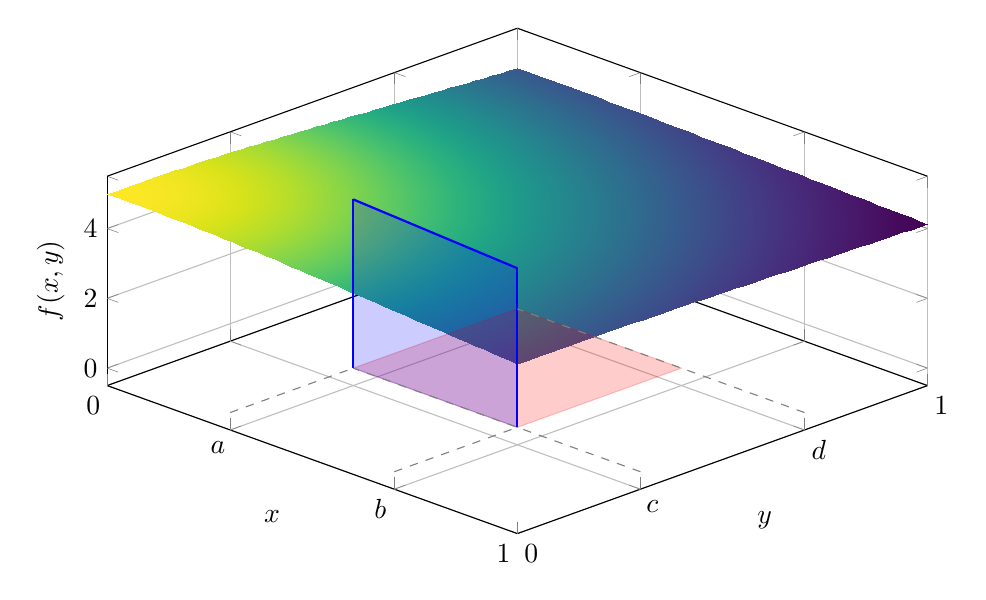
\begin{tikzpicture}
    \begin{axis}[
        view={45}{45},
        xlabel={$x$},
        ylabel={$y$},
        zlabel={$f(x,y)$},
        xtick={0,1},
        ytick={0,1},
        xticklabels={$0$,$1$},
        yticklabels={$0$,$1$},
        extra x ticks={0.3, 0.7},
        extra x tick labels={$a$,$b$},
        extra y ticks={0.3, 0.7},
        extra y tick labels={$c$,$d$},
        domain=0:1,
        y domain=0:1,
        samples=50,
        samples y=50,
        grid=major,
        width=12cm,
        height=8cm,
        colormap/viridis
    ]
        % Plot the lifted surface
        \addplot3[surf, shader=interp] {exp(-x^2-y^2) + 4};
        
        % Red shaded footprint
        \addplot3[red, fill=red, opacity=0.2] coordinates {
            (0.3, 0.3, 0)
            (0.7, 0.3, 0)
            (0.7, 0.7, 0)
            (0.3, 0.7, 0)
            (0.3, 0.3, 0)
        };
        
        % Blue shaded region between blue vertical poles
        \addplot3[blue, fill=blue, opacity=0.2] coordinates {
            (0.3, 0.3, 0)
            (0.3, 0.3, 4.835270)
            (0.7, 0.3, 4.559898)
            (0.7, 0.3, 0)
            (0.3, 0.3, 0)
        };
        
        % Blue vertical lines from (a, c) and (b, c) to the function
        \addplot3[blue, thick] coordinates {(0.3, 0.3, 0) (0.3, 0.3, 4.835270)};
        \addplot3[blue, thick] coordinates {(0.7, 0.3, 0) (0.7, 0.3, 4.559898)};
        
        % Connect the blue lines along y = c at the function
        \addplot3[blue, thick] coordinates {(0.3, 0.3, 4.835270) (0.7, 0.3, 4.559898)};
        
        % Dotted lines from footprint to the y-axis
        \addplot3[gray, dashed] coordinates {(0.3, 0, 0) (0.3, 0.3, 0)};
        \addplot3[gray, dashed] coordinates {(0.7, 0, 0) (0.7, 0.3, 0)};
        \addplot3[gray, dashed] coordinates {(1, 0.3, 0) (0.3, 0.3, 0)};
        \addplot3[gray, dashed] coordinates {(1, 0.7, 0) (0.3, 0.7, 0)};
    \end{axis}
\end{tikzpicture}
\caption{\textit{Just as multiplying $\ell \times w \times h$ produces Volume the same way $w \times h \times \ell$ does, Fubini's theorem lets you calculate the volume under the curve commutatively. In this figure, we could either multiply the blue region (representing integration along $x$ at a fixed $y=c$) over the range of $y$ from $c$ to $d$, or the red region (representing integration along $y$ at a fixed $x$ between $a$ and $b$) over the range of $x$ from $a$ to $b$. Both approaches yield the same total volume under the surface.}}
\end{figure}

\subsubsection*{Understanding Iterated Integrals} \index{Iterated Integrals}

\noindent Let's examine the first form of Fubini's Theorem in detail:
\[
\int_a^b \left[\int_c^d f(x,y) \, dy\right] dx
\]

\noindent This is called an iterated integral, and we evaluate it from the inside out:

\begin{enumerate}
   \item First, compute the inner integral $\displaystyle\int_c^d f(x,y) \, dy$:
       \begin{itemize}
           \item Treat $x$ as a constant
           \item Integrate with respect to $y$ from $c$ to $d$
           \item The result will be a function of $x$ only
       \end{itemize}
   \item Then, integrate this result with respect to $x$ from $a$ to $b$
\end{enumerate}

\noindent Think of this process as:
\begin{itemize}
   \item First finding the area under the curve for each fixed $x$-value (the inner integral)
   \item Then accumulating these areas as $x$ varies from $a$ to $b$ (the outer integral)
\end{itemize}

\exampleline
\begin{example}
Evaluate each of the following double integrals:
\begin{enumerate}
   \item \(\displaystyle\iint_R xy \,dA\) where $R = [0,2] \times [0,3]$
   \item \(\displaystyle\iint_R (x^3\sqrt{y} + \cos x) \,dA\) where $R = [0,1] \times [0,4]$
   \item \(\displaystyle \iint_{R_3} \frac{1}{1 + x^2 - y^2 - x^2 y^2}\,dA\) where \(R_3 = [0,1]\times\bigl[0,\tfrac12\bigr].\)
\end{enumerate}

\begin{solution}
Let's solve these systematically using Fubini's Theorem.

\begin{enumerate}
\item For \(\displaystyle\iint_R xy \,dA\) on $R = [0,2] \times [0,3]$:
\begin{align*}
\iint_R xy \,dA &= \int_0^2 \left[\int_0^3 xy \,dy\right] dx \\
&= \int_0^2 \left[x\left(\frac{y^2}{2}\right)\right]_0^3 dx \\
&= \int_0^2 \left(\frac{9x}{2}\right) dx \\
&= \frac{9}{2}\left(\frac{x^2}{2}\right)\bigg|_0^2 \\
&= \frac{9}{2}(2) = 9
\end{align*}

\item For \(\displaystyle\iint_R (x^3\sqrt{y} + \cos x) \,dA\) on $R = [0,1] \times [0,4]$:
\begin{align*}
\iint_R (x^3\sqrt{y} + \cos x) \,dA &= \int_0^1 \left[\int_0^4 (x^3\sqrt{y} + \cos x) \,dy\right] dx \\
&= \int_0^1 \left[x^3\left(\frac{2y^{3/2}}{3}\right) + y\cos x\right]_0^4 dx \\
&= \int_0^1 \left(\frac{16x^3}{3} + 4\cos x\right) dx \\
&= \left[\frac{16x^4}{12} + 4\sin x\right]_0^1 \\
&= \frac{16}{12} + 4\sin(1) \\
&= \frac{4}{3} + 4\sin(1)
\end{align*}

\item For \(\displaystyle\iint_R \frac{1}{1 + x^2 - y^2 - x^2y^2} \,dA\) on $R = [0,1] \times [0,\frac{1}{2}]$:

First, notice the denominator factors:
\[
1 + x^2 - y^2 - x^2y^2 = (1 + x^2)(1 - y^2)
\]
Therefore:
\begin{align*}
\iint_R \frac{1}{1 + x^2 - y^2 - x^2y^2} \,dA &= \int_0^1 \left[\int_0^{1/2} \frac{1}{(1+x^2)(1-y^2)} \,dy\right] dx \\
&= \int_0^1 \frac{1}{1+x^2}\left[\text{arctanh}(y)\right]_0^{1/2} dx \\
&= \int_0^1 \frac{\text{arctanh}(1/2)}{1+x^2} dx \\
&= \text{arctanh}(1/2)\left[\arctan(x)\right]_0^1 \\
&= \text{arctanh}(1/2)\cdot\frac{\pi}{4}
\end{align*}
\end{enumerate}
\end{solution}
\end{example}
\exampleline

\subsubsection*{Strategic Choice of Integration Order}

\noindent While Fubini's Theorem guarantees both orders of integration give the same result, one order might be significantly simpler than the other. In fact, sometimes one order might be straightforward while the other becomes extremely difficult or even impossible to evaluate directly. Let's develop some strategies for choosing the optimal order of integration. \\ \\ A systematic approach to choosing integration order involves:

\begin{enumerate}
   \item \textbf{Examine the Function Structure:}
       \begin{itemize}
           \item Look for terms that would simplify if held constant
           \item Identify potential partial fraction decompositions
           \item Note any terms that might lead to easier substitutions
       \end{itemize}
   
   \item \textbf{Consider the Integration Boundaries:}
       \begin{itemize}
           \item Check which variable has simpler limits
           \item Look for limits that depend on the other variable
           \item Consider whether one set of limits might introduce new complications
       \end{itemize}
   
   \item \textbf{Anticipate the Result of Each Integration:}
       \begin{itemize}
           \item Consider what antiderivatives would arise in each order
           \item Look for potential simplifications in the resulting functions
           \item Watch for terms that might cancel or combine nicely
       \end{itemize}
\end{enumerate}

\noindent Let's examine some specific scenarios:

\begin{itemize}
   \item When $f(x,y)$ contains $e^x$ or $\ln(x)$, integrate with respect to $y$ first to keep these terms ``constant"
   \item For rational functions like $\frac{1}{(x^2+y^2)}$, consider which variable might lead to easier partial fractions
   \item If $f(x,y)$ factors as $g(x)h(y)$, either order works equally well
\end{itemize}

\noindent Common pitfalls to avoid:
\begin{itemize}
   \item Don't automatically choose the order that makes the inner integral look simpler—consider the full process
   \item Watch for cases where simplifying the inner integral makes the outer integral more complicated
   \item Be careful with functions that might become undefined during integration
\end{itemize}

\noindent Consider this example: If we have
\[
\iint_R \frac{y}{x^2+y^2} \,dA
\]
integrating with respect to $y$ first leads to arctangent functions, while integrating with respect to $x$ first leads to logarithms. Depending on the region $R$, one approach might be significantly easier than the other. \\ \\ The key insight is that Fubini's Theorem gives us flexibility in our approach. By choosing the optimal order of integration, we can often transform a seemingly difficult double integral into a sequence of manageable single integrals. This exemplifies a broader principle in mathematics: when faced with a complex problem, look for ways to transform it into a sequence of simpler, familiar problems.


\exampleline
\begin{example}
Evaluate \(\displaystyle\iint_R \frac{y}{x^2 + y^2} \,dA\) where $R = [1,2] \times [-1,1]$ by considering both orders of integration. Determine which approach is more efficient.

\begin{solution}
Let's evaluate this integral using both possible orders to compare approaches. \\ \\ First, let's try integrating with respect to $y$ first:
\[
\iint_R \frac{y}{x^2 + y^2} \,dA = \int_1^2 \int_{-1}^1 \frac{y}{x^2 + y^2} \,dy\,dx
\]

\noindent For any fixed $x$, notice that the integrand $f(y) = \frac{y}{x^2 + y^2}$ is an odd function in $y$:
\[
f(-y) = \frac{-y}{x^2 + (-y)^2} = -\frac{y}{x^2 + y^2} = -f(y)
\]

\noindent Therefore, when integrating over the symmetric interval $[-1,1]$:
\[
\int_{-1}^1 \frac{y}{x^2 + y^2} \,dy = 0
\]
 \noindent since the negative area perfectly cancels the positive area. Thus:
\[
\iint_R \frac{y}{x^2 + y^2} \,dA = \int_1^2 [0] \,dx = 0
\]

\noindent Now, let's examine what happens if we integrate with respect to $x$ first:
\[
\iint_R \frac{y}{x^2 + y^2} \,dA = \int_{-1}^1 \int_1^2 \frac{y}{x^2 + y^2} \,dx\,dy
\]

\noindent Here, $y$ is held constant in the inner integral:
\[
\int_1^2 \frac{y}{x^2 + y^2} \,dx
\]

\noindent For fixed \( y \neq 0 \), we use the standard arctangent formula:
\[
\int \frac{y}{x^2 + y^2} \, dx = \arctan\!\left(\frac{x}{y}\right)
\]

\noindent Evaluating from $x = 1$ to $x = 2$ and then integrating with respect to $y$ becomes quite involved:
\[
\int_{-1}^1 y\left[\frac{1}{|y|}\arctan\left(\frac{x}{y}\right)\right]_{x=1}^{x=2} dy
\]
\begin{figure}[H]
\centering
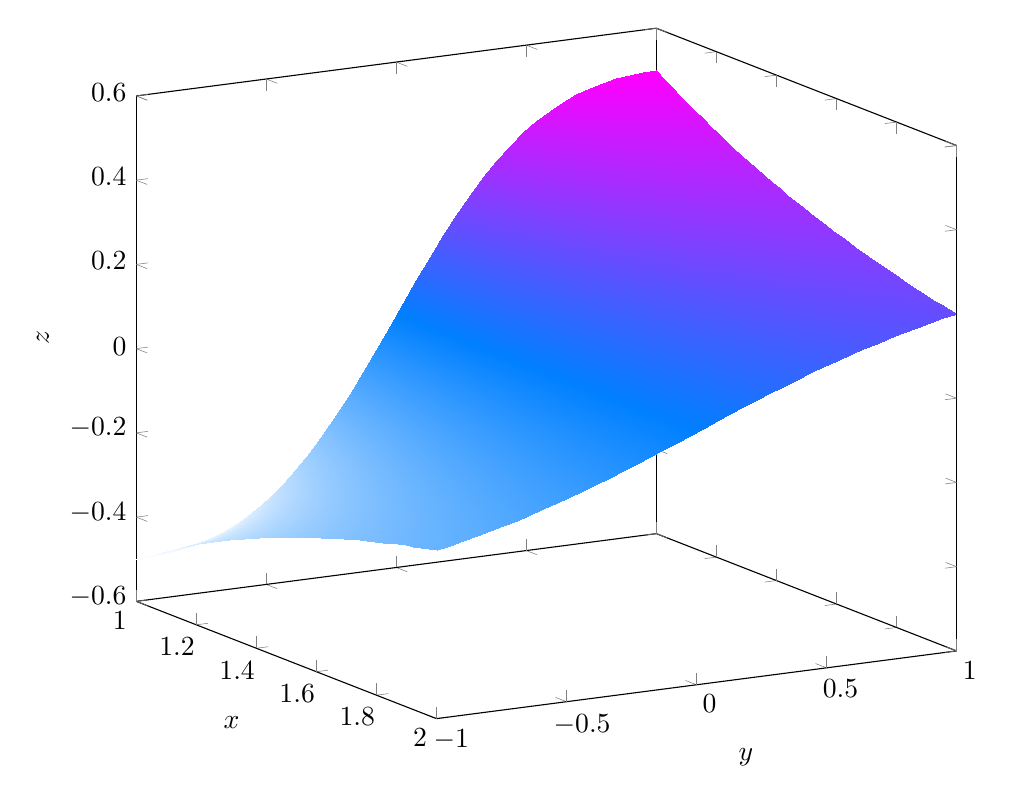
\begin{tikzpicture}
\begin{axis}[
    width=12cm,
    view={60}{15},  % <-- elevation of 15 for a slight overhead perspective
    domain=1:2,
    y domain=-1:1,
    xmin=1, xmax=2,
    ymin=-1, ymax=1,
    samples=40,
    samples y=40,
    xlabel={$x$},
    ylabel={$y$},
    zlabel={$z$},
    colormap/cool,
    mesh/ordering=y varies,
    mesh/cols=40
]
\addplot3[
    surf,
    shader=interp
]
{y/(x^2 + y^2)};
\end{axis}
\end{tikzpicture}
\caption{\textit{A plot of the function $f(x,y) = \frac{y}{x^2 + y^2}$. Notice that the function is odd in $y$, and thus integrating across symmetric bounds produces volume equal to 0.}}
\end{figure}
\end{solution}
\end{example}
\exampleline

\subsubsection*{Indefinite Double Integration} \index{Indefinite Double Integration}

Just as with single integrals, we can consider indefinite double integrals where we seek a function $F(x,y)$ such that:
\[
\frac{\partial^2 F}{\partial x\partial y} = g(x,y)
\]

\noindent First, integrate with respect to \( y \):
\[
\frac{\partial F}{\partial x} = \int g(x, y) \, dy = G(x, y) + p(x),
\]
where \( G(x, y) = \int g(x, y) \, dy \) and \( p(x) \) is an arbitrary function of \( x \). \\

\noindent Next, integrate with respect to \( x \):
\[
F(x, y) = \int \frac{\partial F}{\partial x} \, dx = \int G(x, y) \, dx + \int p(x) \, dx + q(y).
\]

\noindent The general solution is:
\[
F(x, y) = H(x, y) + P(x) + q(y),
\]
where \( H(x, y) = \int G(x, y) \, dx \), \( P(x) = \int p(x) \, dx \), and \( q(y) \) is an arbitrary function of \( y \). \\
\noindent You have heard in your Calculus I and II texts that finding the function from an expression of derivatives is called a Differential Equation. This is the multivariable analog of that, called Partial Differential Equations, which will be introduced and discussed further in Chapter 6. \\

\noindent To find indefinite double integrals:
\begin{enumerate}
   \item First integrate with respect to one variable, adding an arbitrary function of the other variable
   \item Then integrate the result with respect to the second variable
   \item Combine all arbitrary terms into the general form above
\end{enumerate}

\noindent For example, if $f(x,y) = xy$:
\begin{align*}
\iint xy \,dx\,dy &= \int\left(\int xy \,dx\right)\,dy \\
&= \int\left(\frac{x^2y}{2} + h(y)\right)\,dy \\
&= \frac{x^2y^2}{4} + \int h(y)\,dy + g(x) \\
&= \frac{x^2y^2}{4} + g(x) + H(y)
\end{align*}

\noindent This process highlights the additional complexity that arises in multivariable calculus—instead of just a constant of integration, we now have arbitrary functions to consider. Let's hit a couple of examples:

\exampleline
\begin{example}
Find the indefinite double integral for:
\begin{enumerate}
   \item \(\displaystyle \iint xy^2 \,dx\,dy\)
   \item \(\displaystyle \iint (x^2 + 3xy) \,dx\,dx\) \quad (i.e., integrate twice with respect to \(x\))
\end{enumerate}

\begin{solution}
Let's solve each integral systematically, remembering that for indefinite double integrals we need to include arbitrary functions of the other variable at each step.

\begin{enumerate}
\item For \(\displaystyle \iint xy^2 \,dx\,dy\):
\begin{align*}
\int xy^2 \,dx &= \frac{x^2y^2}{2} + h(y) \\[1ex]
\iint xy^2 \,dx\,dy &= \int \left(\frac{x^2y^2}{2} + h(y)\right) dy \\[1ex]
&= \frac{x^2y^3}{6} + \int h(y)\,dy + g(x) \\[1ex]
&= \frac{x^2y^3}{6} + g(x) + H(y)
\end{align*}
where $g(x)$ and $H(y)$ are arbitrary functions.

\item For \(\displaystyle \iint (x^2 + 3xy) \,dx^2\):

First, note that integrating with respect to $dx^2$ means we integrate twice with respect to $x$:
\begin{align*}
\int (x^2 + 3xy) \,dx &= \frac{x^3}{3} + \frac{3x^2y}{2} + h_1(y) \\[1ex]
\int \left(\frac{x^3}{3} + \frac{3x^2y}{2} + h_1(y)\right) \,dx &= \frac{x^4}{12} + \frac{x^3y}{2} + h_1(y)x + h_2(y) \\[1ex]
\end{align*}
\end{enumerate}
\end{solution}
\end{example}
\exampleline





\newpage




\lecture{Double Integrals over General Regions} \index{General Regions}

\noindent The world rarely presents us with perfectly rectangular regions to integrate over. Whether we're computing fluid flow through an irregular pipe, finding the center of mass of a non-rectangular plate, or calculating heat distribution across a circular disk, we need tools to handle integration over more general regions. In this lecture, we extend our understanding of double integrals beyond rectangular boundaries to tackle these real-world scenarios.

\begin{figure}[H]
\centering
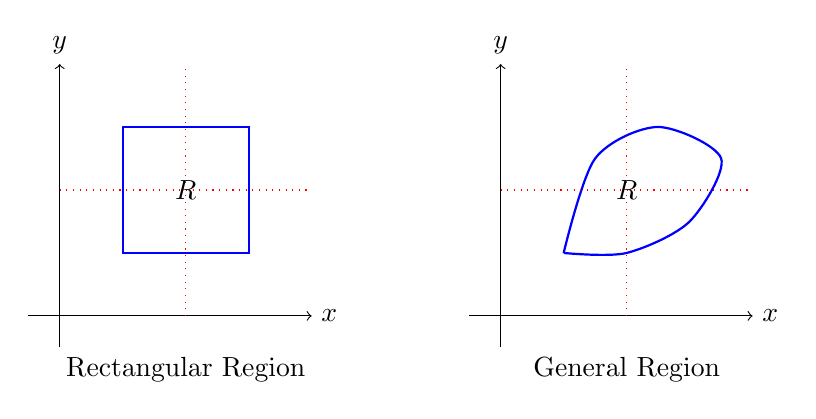
\begin{tikzpicture}[scale=0.8]
% First subplot - Rectangular region
\begin{scope}[local bounding box=plot1]
    % Draw axes
    \draw[->] (-0.5,0) -- (4,0) node[right] {$x$};
    \draw[->] (0,-0.5) -- (0,4) node[above] {$y$};
    
    % Draw rectangle
    \draw[thick, blue] (1,1) rectangle (3,3);
    
    % Sample lines
    \draw[red, dotted] (2,0) -- (2,4);
    \draw[red, dotted] (0,2) -- (4,2);
    
    % Label
    \node at (2,2) {$R$};
    \node[below] at (2,-0.5) {Rectangular Region};
\end{scope}

% Second subplot - General region 
\begin{scope}[xshift=7cm, local bounding box=plot2] 
    % Draw axes 
    \draw[->] (-0.5,0) -- (4,0) node[right] {$x$}; 
    \draw[->] (0,-0.5) -- (0,4) node[above] {$y$}; 
    
    % Draw curved region (without self-intersection)
    \draw[thick, blue] plot[smooth] coordinates {(1,1) (1.5,2.5) (2.5,3) (3.5,2.5) (3,1.5) (2,1) (1,1)}; 
    
    % Sample lines 
    \draw[red, dotted] (2,0) -- (2,4); 
    \draw[red, dotted] (0,2) -- (4,2); 
    
    % Label 
    \node at (2,2) {$R$}; 
    \node[below] at (2,-0.5) {General Region}; 
\end{scope}
\end{tikzpicture}
\caption{\textit{Left: A rectangular region where the bounds of integration are constant. Right: A general region where the bounds may vary along each coordinate direction.}}
\label{fig:region_comparison}
\end{figure}


\noindent Just as we first mastered integration over intervals before handling more complex single-variable integration, our study of rectangular regions has prepared us for this natural generalization. The key insight is that while our regions may now have curved boundaries, our fundamental approach remains the same—we still aim to accumulate infinitesimal pieces over a region systematically.





\begin{figure}[H]
\centering
\tdplotsetmaincoords{70}{110}
\begin{tikzpicture}[tdplot_main_coords, line cap=round, >=stealth, scale=1.5,
declare function={
    surfacefn(\x,\y)=2+0.2*sin(90*\x)*cos(90*\y);
}]
% Axes
\draw[->] (0,0,0) coordinate (O) -- (4,0,0) node[pos=1.05]{$x$};
\draw[->] (O) -- (0,4,0) node[pos=1.05]{$y$};
\draw[->] (O) -- (0,0,3) node[pos=1.05]{$z$};

% Surface mesh (for entire plot with thicker lines)
\foreach \x in {0,0.5,...,3.5} {
    \draw[blue!70,thick,opacity=0.7] plot[variable=\y,domain=0:3.5,samples=30]
    (\x,\y,{surfacefn(\x,\y)});
}
\foreach \y in {0,0.5,...,3.5} {
    \draw[blue!70,thick,opacity=0.7] plot[variable=\x,domain=0:3.5,samples=30]
    (\x,\y,{surfacefn(\x,\y)});
}

% Region boundary (non-square region in Cartesian coordinates)
\draw[red,thick] plot[smooth cycle, tension=0.8] coordinates {
    (1,1,0)
    (1.8,1.2,0)
    (2.5,2,0)
    (2,3,0)
    (1.2,2.5,0)
    (1,1,0)
}; % Ensure proper cycle closure

% Vertical edges connecting region boundary to the surface
\foreach \pt/\xp/\yp in {
    (1,1)/1/1,
    (1.8,1.2)/1.8/1.2,
    (2.5,2)/2.5/2,
    (2,3)/2/3,
    (1.2,2.5)/1.2/2.5
} {
    \pgfmathsetmacro{\z}{surfacefn(\xp,\yp)} % Use \xp and \yp for calculations
    \draw[gray, dotted, thick] \pt -- (\xp,\yp,\z); % Ensure proper TikZ syntax
}

% Fill region on surface
\fill[blue!30,opacity=0.6]
plot[smooth cycle, tension=0.8] coordinates {
    (1,1,{surfacefn(1,1)})
    (1.8,1.2,{surfacefn(1.8,1.2)})
    (2.5,2,{surfacefn(2.5,2)})
    (2,3,{surfacefn(2,3)})
    (1.2,2.5,{surfacefn(1.2,2.5)})
    (1,1,{surfacefn(1,1)})
}; % Ensure proper closure

% Adding labels for h(x,y) and the region R
\node[blue] at (2.5,2,3.2) {$h(x,y)$};
\node[red] at (1.5,2,0) {$R$};

\end{tikzpicture}
\caption{\textit{A visualization of a double integral over a region \( R \), with the surface \( h(x,y) \) shown above.}}
\end{figure}


\subsection*{Type I and Type II Regions} \index{Double Integral Regions}  

\noindent When moving beyond rectangular regions, our first task is to understand how to describe more general regions mathematically. In rectangular regions, our bounds of integration were constants—fixed numbers that defined our region's boundaries. Now, these bounds might be functions, describing curves that trace out our region's boundaries. This transition from constant to variable bounds represents a fundamental shift in how we must think about setting up our integrals. \\ \\
Let's develop a systematic approach for analyzing these general regions and determining their bounds of integration. Just as we used the interval $[a,b]$ to precisely define the domain of a single integral, we now need two sets of bounds to fully describe our region of integration.





\subsubsection*{Analyzing Region Types}

\noindent Before we can set up a double integral over a general region, we must first analyze the region's geometry to determine whether it's more naturally described as Type I or Type II. This analysis involves examining how the region's boundaries intersect with horizontal and vertical lines. \\

\noindent For any given region $R$, ask yourself:
\begin{enumerate}
    \item Can any vertical line through the region intersect the boundary at most twice?
    \item Can any horizontal line through the region intersect the boundary at most twice?
    \item Are these intersections continuous functions of position?
\end{enumerate}

\noindent If the answer to the first question is ``yes," the region can be described as Type I. If the answer to the second question is ``yes," it can be described as Type II. Some regions can be described as both Type I and Type II, giving us flexibility. However, some regions---such as annular regions---cannot be described as either type, since vertical and horizontal lines may cross the boundary more than twice. In such cases, we must split the region into simpler pieces or switch coordinate systems.


\begin{figure}[H]
    \centering
    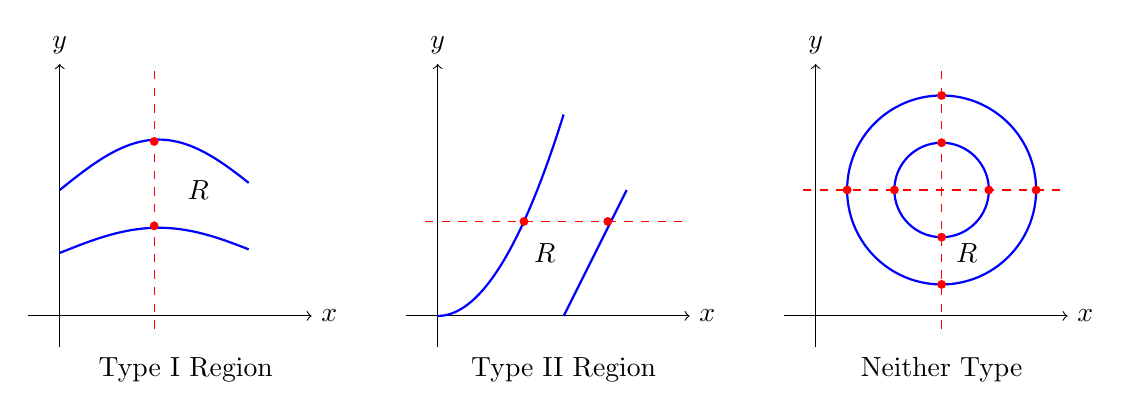
\begin{tikzpicture}[scale=0.8]
        % First subplot - Type I region
        \begin{scope}[local bounding box=plot1]
            % Draw axes
            \draw[->] (-0.5,0) -- (4,0) node[right] {$x$};
            \draw[->] (0,-0.5) -- (0,4) node[above] {$y$};
            
            % Draw curves - using proper scaling for trig functions
            \draw[thick, blue] plot[smooth, domain=0:3] (\x, {2 + 0.8*sin(\x r)});
            \draw[thick, blue] plot[smooth, domain=0:3] (\x, {1 + 0.4*sin(\x r)});
            
            % Sample vertical line at x = 1.5
            \draw[dashed, red] (1.5,-0.2) -- (1.5,4);
            
            % Intersection points
            \fill[red] (1.5,2.77) circle (2pt);
            \fill[red] (1.5,1.43) circle (2pt);
            
            \node at (2.2,2) {$R$};
            \node[below] at (2,-0.5) {Type I Region};
        \end{scope}
        
        % Second subplot - Type II region
        \begin{scope}[xshift=6cm, local bounding box=plot2]
            % Draw axes
            \draw[->] (-0.5,0) -- (4,0) node[right] {$x$};
            \draw[->] (0,-0.5) -- (0,4) node[above] {$y$};
            
            % Draw curves - using simpler quadratic and linear functions
            \draw[thick, blue] plot[domain=0:2, samples=50] (\x, {0.8*\x*\x});
            \draw[thick, blue] plot[domain=0:2, samples=50] ({2 + 0.5*\x}, \x);
            
            % Sample horizontal line
            \draw[dashed, red] (-0.2,1.5) -- (4,1.5);
            
            % Intersection points
            \fill[red] (1.37,1.5) circle (2pt);
            \fill[red] (2.7,1.5) circle (2pt);
            
            \node at (1.7,1) {$R$};
            \node[below] at (2,-0.5) {Type II Region};
        \end{scope}
        
        % Third subplot - Neither type (concentric circles)
        \begin{scope}[xshift=12cm, local bounding box=plot3]
            % Draw axes
            \draw[->] (-0.5,0) -- (4,0) node[right] {$x$};
            \draw[->] (0,-0.5) -- (0,4) node[above] {$y$};
            
            % Concentric circles
            \draw[thick, blue] (2,2) circle (1.5);
            \draw[thick, blue] (2,2) circle (0.75);
            
            % Sample lines
            \draw[dashed, red] (2,-0.2) -- (2,4);
            \draw[dashed, red] (-0.2,2) -- (4,2);
            
            % Intersection points
            \foreach \y in {0.5,1.25,2.75,3.5} {
                \fill[red] (2,\y) circle (2pt);
            }
            \foreach \x in {0.5,1.25,2.75,3.5} {
                \fill[red] (\x,2) circle (2pt);
            }
            
            \node at (2.4,1) {$R$};
            \node[below] at (2,-0.5) {Neither Type};
        \end{scope}
        

    \end{tikzpicture}
    \caption{\textit{Examples of regions and their classifications based on line intersections. Left: Type I region showing exactly two intersections with any vertical line. Center: Type II region showing exactly two intersections with any horizontal line. Right: An annular region that cannot be described as either type since both vertical and horizontal lines can intersect the boundary more than twice.}}
    \label{fig:region_types}
\end{figure}

\subsubsection*{Type I Regions: Vertical Slicing} \index{Double Integral Regions!Type I Regions}

\noindent A region $R$ in the $xy$-plane is called a \textbf{Type I region} if it can be described as:
\[
R = \{(x,y) : a \leq x \leq b, \quad g_1(x) \leq y \leq g_2(x)\}
\]
where $g_1(x)$ and $g_2(x)$ are continuous functions on $[a,b]$. \\

\noindent To determine the bounds for a Type I region, first and foremost we must sketch the region $R$. A clear diagram is absolutely essential—it helps us visualize the intersection points and understand how the bounds will be structured. Once we have our diagram, we follow these steps:

\begin{enumerate}
    \item Identify the left and right bounds ($a$ and $b$). These are typically intersection points of boundary curves or points where vertical tangent lines occur.
    
    \item At any fixed $x$-value in $[a,b]$, determine where a vertical line enters and exits the region—these become $g_1(x)$ and $g_2(x)$ respectively.
    
    \item Write these entry and exit points as functions of $x$. These become our inner bounds of integration.
\end{enumerate}

\noindent Let's see this process in action with an example:

\exampleline
\begin{example}
Find the bounds needed to evaluate \(\displaystyle\iint_R f(x,y) \,dA\) where $R$ is bounded below by $y = x^2$ and above by $y = 4-x^2$.

\begin{solution}
Let's first sketch the region $R$ to visualize our domain of integration:

\begin{center}
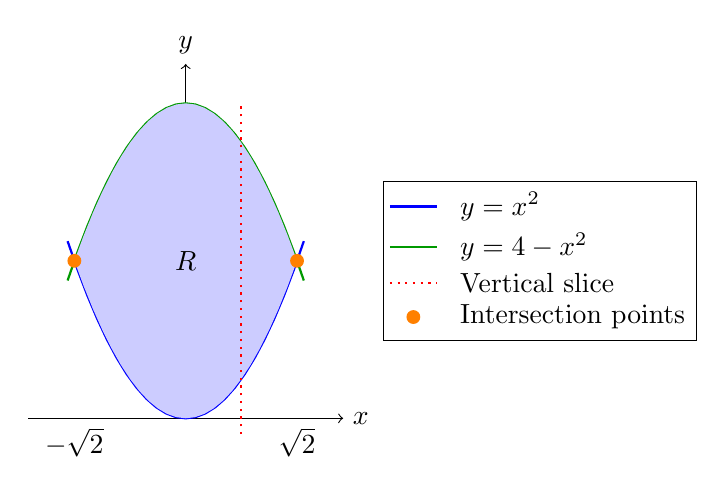
\begin{tikzpicture}[scale=1]
% Draw axes
\draw[->] (-2,0) -- (2,0) node[right] {$x$};
\draw[->] (0,0) -- (0,4.5) node[above] {$y$};

% Draw parabolas
\draw[blue, thick, domain=-1.5:1.5] plot (\x, {\x*\x});
\draw[green!60!black, thick, domain=-1.5:1.5] plot (\x, {4-\x*\x});

% Fill region
\fill[blue!20] plot[domain=-1.414:1.414] (\x, {\x*\x}) --
plot[domain=1.414:-1.414] (\x, {4-\x*\x}) -- cycle;

% Sample vertical line
\draw[red, dotted, thick] (0.7,-0.2) -- (0.7,4);

% Intersection points
\fill[orange] (1.414,2) circle (2.5pt);
\fill[orange] (-1.414,2) circle (2.5pt);

% Region label
\node at (0,2) {$R$};

% Points of intersection on x-axis
\node[below] at (1.414,0) {$\sqrt{2}$};
\node[below] at (-1.414,0) {$-\sqrt{2}$};

% Legend with matrix for automatic spacing
\matrix [draw=black, fill=white, inner sep=0.2em, row sep=0.05em, column sep=0.6em,
         anchor=west] at (2.5,2)
{
    \draw[blue, thick] (0,0) -- (0.6,0); & \node[align=left] {$y = x^2$}; \\
    \draw[green!60!black, thick] (0,0) -- (0.6,0); & \node[align=left] {$y = 4-x^2$}; \\
    \draw[red, dotted, thick] (0,0) -- (0.6,0); & \node[align=left] {Vertical slice}; \\
    \fill[orange] (0.3,0) circle (2.5pt); & \node[align=left] {Intersection points}; \\
};

\end{tikzpicture}
\end{center}

To find the bounds, we first determine where the curves intersect:
\[
x^2 = 4-x^2 \implies 2x^2 = 4 \implies x = \pm\sqrt{2}
\]

From our sketch, we can see:
\begin{itemize}
   \item The region extends from $x = -\sqrt{2}$ to $x = \sqrt{2}$
   \item For each $x$ in this interval, $y$ ranges from $x^2$ to $4-x^2$
\end{itemize}

Therefore:
\[
\iint_R f(x,y) \,dA = \int_{-\sqrt{2}}^{\sqrt{2}} \int_{x^2}^{4-x^2} f(x,y) \,dy\,dx
\]

\noindent Note how the sketch clearly shows this is a Type I region, as any vertical line (like our dashed sample line) intersects the boundary curves exactly twice. At this point we may now proceed with integrating as we have done in the previous lecture.
\end{solution}
\end{example}

\exampleline
\begin{example}
A manufacturer produces some eccentric-looking solar panels whose efficiency varies with position. The usable surface of each panel is bounded below by $y = \sin(x)$ and above by $y = 2 + \cos(x)$ for $x \in [0,2\pi]$. If the efficiency at any point $(x,y)$ is given by $E(x,y) = \frac{1}{80} x^2y$, find the average efficiency over the entire panel.

\begin{solution}
Let's first sketch the region to understand our domain of integration:
\begin{center}
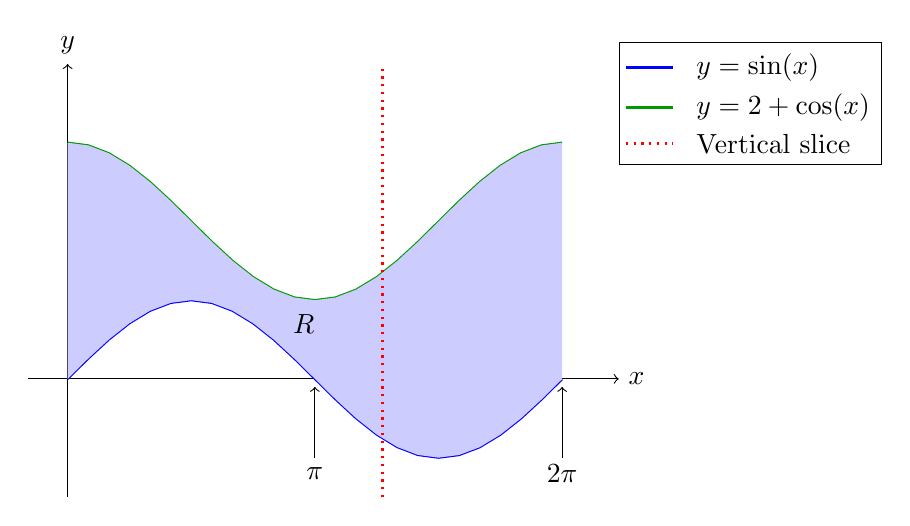
\begin{tikzpicture}[scale=1]
% Draw axes
\draw[->] (-0.5,0) -- (7,0) node[right] {$x$};
\draw[->] (0,-1.5) -- (0,4) node[above] {$y$};

% Draw curves
\draw[blue, thick, domain=0:6.28] plot (\x, {sin(\x r)});
\draw[green!60!black, thick, domain=0:6.28] plot (\x, {2 + cos(\x r)});

% Fill region
\fill[blue!20] plot[domain=0:6.28] (\x, {sin(\x r)}) --
plot[domain=6.28:0] (\x, {2 + cos(\x r)}) -- cycle;

% Sample vertical line
\draw[red, dotted, thick] (4,-1.5) -- (4,4);

% Region label
\node at (3,0.7) {$R$};

% Pi markers with arrows
\draw[->] (3.14,-1) -- (3.14,-0.1);
\draw[->] (6.28,-1) -- (6.28,-0.1);
\node at (3.14,-1.2) {$\pi$};
\node at (6.28,-1.2) {$2\pi$};

% Legend moved to top right
\matrix [draw=black, fill=white, inner sep=0.2em, row sep=0.05em, column sep=0.6em, anchor=west] at (7,3.5) {
\draw[blue, thick] (0,0) -- (0.6,0); & \node[align=left] {$y = \sin(x)$}; \\
\draw[green!60!black, thick] (0,0) -- (0.6,0); & \node[align=left] {$y = 2 + \cos(x)$}; \\
\draw[red, dotted, thick] (0,0) -- (0.6,0); & \node[align=left] {Vertical slice}; \\
};
\end{tikzpicture}
\end{center}

\noindent To find the average efficiency, we need:
\begin{align*}
E_{\text{avg}}
&= \frac{\iint_R E(x,y) \, dA}{\iint_R \, dA} \\
&= \frac{\iint_R \frac{1}{80} x^2 y \, dA}{\text{Area of } R}.
\end{align*}

\noindent From the bounds, we have $0 \le x \le 2\pi$ and $\sin(x) \le y \le 2 + \cos(x)$. Thus,
\[
\iint_R x^2y \, dA
= \int_{0}^{2\pi} \int_{\sin(x)}^{2+\cos(x)}  \frac{1}{80} x^2y \, dy \, dx.
\]

\noindent Evaluate the inner integral:
\begin{align*}
\int_{\sin(x)}^{2+\cos(x)} \frac{1}{80} x^2y \, dy 
&= \frac{x^2}{80} \left[ \frac{y^2}{2} \right]_{y=\sin(x)}^{y=2 + \cos(x)} \\
&= \frac{x^2}{160} \Bigl( (2 + \cos(x))^2 \;-\; \sin^2(x) \Bigr).
\end{align*}

\noindent Thus,
\begin{align*}
\iint_R x^2y \, dA
&= \frac{1}{160} \int_{0}^{2\pi} x^2 \bigl( 4 + 4\cos(x) + \cos(2x) \bigr) \, dx \\
&= \frac{1}{160} \Bigl(
4 \int_{0}^{2\pi} x^2 \, dx
\;+\;
4 \int_{0}^{2\pi} x^2 \cos(x) \, dx
\;+\;
\int_{0}^{2\pi} x^2 \cos(2x) \, dx
\Bigr).
\end{align*}

\noindent By standard integration techniques,
\[
\int_{0}^{2\pi} x^2 \, dx \;=\; \frac{8\pi^3}{3},
\quad
\int_{0}^{2\pi} x^2 \cos(x) \, dx \;=\; 4\pi,
\quad
\int_{0}^{2\pi} x^2 \cos(2x) \, dx \;=\; \pi.
\]

\noindent Hence,
\begin{align*}
\iint_R \frac{1}{80} x^2 y \, dA
&= \frac{1}{160}
\Bigl( 4\cdot\frac{8\pi^3}{3} \;+\; 4\cdot 4\pi \;+\; \pi \Bigr) \\
&= \frac{1}{160}
\Bigl( \frac{32\pi^3}{3} + 16\pi + \pi \Bigr)
\end{align*}

\noindent Next, the area of $R$ is
\begin{align*}
\text{Area}(R)
&= \int_{0}^{2\pi} \Bigl[\, (2 + \cos(x)) - \sin(x) \Bigr] \, dx \\
&= \int_{0}^{2\pi} 2\,dx + \int_{0}^{2\pi} \cos(x)\,dx - \int_{0}^{2\pi} \sin(x)\,dx \\
&= 4\pi.
\end{align*}

\noindent Therefore, the average efficiency is
\begin{align*}
E_{\text{avg}}
&= \frac{\frac{1}{160}
\Bigl( \frac{32\pi^3}{3} + 16\pi + \pi \Bigr)}{4\pi} \approx 0.191 = 19.1 \%.
\end{align*}

\noindent This is the average efficiency across the entire solar panel surface. Note that unlike having a surface that intersects the $xy$-plane producing negative volume, the bounds of the region that go to negative quadrants do not affect the volume.
\end{solution}
\end{example}
\exampleline

\subsubsection*{Type II Regions: Horizontal Slicing} \index{Double Integral Regions!Type II Regions}

\noindent A region $R$ in the $xy$-plane is called a \textbf{Type II region} if it can be described as:
\[
R = \{(x,y) : c \leq y \leq d, \quad h_1(y) \leq x \leq h_2(y)\}
\]
where $h_1(y)$ and $h_2(y)$ are continuous functions on $[c,d]$. \\ \\
\noindent Just as with Type I regions, sketching region $R$ is essential. A clear diagram helps us visualize where horizontal lines intersect our boundaries and how to structure our integration. After sketching the region, we follow these steps:

\begin{enumerate}
    \item Identify the bottom and top bounds ($c$ and $d$). These are typically intersection points of boundary curves or points where horizontal tangent lines occur.
    
    \item At any fixed $y$-value in $[c,d]$, determine where a horizontal line enters and exits the region—these become $h_1(y)$ and $h_2(y)$ respectively.
    
    \item Write these entry and exit points as functions of $y$. These become our inner bounds of integration.
\end{enumerate}


\begin{example}
In fluid dynamics, the velocity potential $\phi(x,y) = \frac{x}{1+y^2}$ describes the flow field in a curved channel. Calculate the total potential flux through region $R$ bounded by the cubic barrier $x = y^3$, the vertical wall $x = 4$, and the horizontal barriers at $y = \pm 1$. \\[1em]
\noindent The potential flux across a region is given by:
\[
\Phi = \iint_R \phi(x,y) \,dA.
\]

\begin{solution}
Let's first sketch region $R$ to understand our flow domain:

\begin{center}
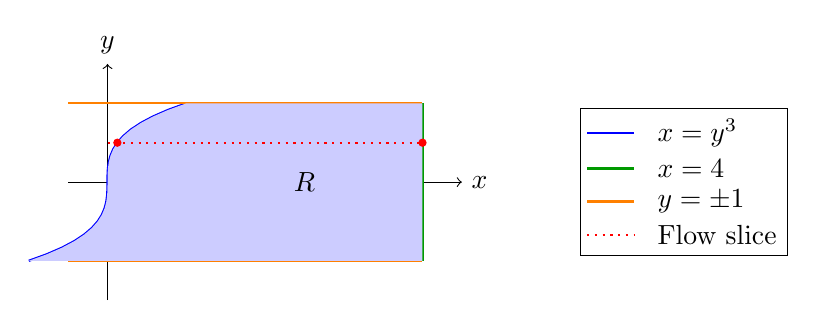
\begin{tikzpicture}[scale=1]
% Draw axes
\draw[->] (-0.5,0) -- (4.5,0) node[right] {$x$};
\draw[->] (0,-1.5) -- (0,1.5) node[above] {$y$};

% Draw curves
\draw[blue, thick, domain=-1:1] plot ({\x*\x*\x}, \x);
\draw[green!60!black, thick] (4,-1) -- (4,1);
\draw[orange, thick] (-0.5,1) -- (4,1);
\draw[orange, thick] (-0.5,-1) -- (4,-1);

% Fill region - only between the curves
\fill[blue!20] plot[domain=-1:1] ({\x*\x*\x}, \x) --
(4,1) -- (4,-1) -- cycle;

% Sample horizontal line
\draw[red, dotted, thick] (0,0.5) -- (4,0.5);

% Region label
\node at (2.5,0) {$R$};

% Horizontal intersection points at y = 0.5
\fill[red] (0.125,0.5) circle (1.5pt);
\fill[red] (4,0.5) circle (1.5pt);

% Legend moved to right
\matrix [draw=black, fill=white, inner sep=0.2em, row sep=0.05em, column sep=0.6em,
anchor=west] at (6,0)
{
\draw[blue, thick] (0,0) -- (0.6,0); & \node[align=left] {$x = y^3$}; \\
\draw[green!60!black, thick] (0,0) -- (0.6,0); & \node[align=left] {$x = 4$}; \\
\draw[orange, thick] (0,0) -- (0.6,0); & \node[align=left] {$y = \pm 1$}; \\
\draw[red, dotted, thick] (0,0) -- (0.6,0); & \node[align=left] {Flow slice}; \\
};
\end{tikzpicture}
\end{center}

\noindent For this flow problem, Type II integration is natural as it aligns with horizontal flow layers. For any fixed $y$-level between $-1$ and $1$, the flow extends from the barrier at $x = y^3$ to the wall at $x = 4$. Therefore:

\begin{align*}
\Phi &= \int_{-1}^{1} \int_{y^3}^{4} \frac{x}{1+y^2}\,dx\,dy \\
&= \int_{-1}^{1} \frac{1}{1+y^2} \left[\frac{x^2}{2}\right]_{y^3}^{4}\,dy \\
&= \int_{-1}^{1} \frac{1}{1+y^2}\!\left(8 - \frac{y^6}{2}\right)\,dy \\
&= 8\int_{-1}^{1} \!\!\frac{dy}{1+y^2}
\;-\;\frac{1}{2}\int_{-1}^{1} \frac{y^6}{1+y^2}\,dy.
\end{align*}

The first integral evaluates to $4\pi$. For the second, using polynomial division:
\begin{align*}
\frac{y^6}{1+y^2} &= y^4 - y^2 + 1 - \frac{1}{1+y^2}, \\
\int_{-1}^{1} \frac{y^6}{1+y^2}\,dy &= \Bigl[\tfrac{y^5}{5} \;-\;\tfrac{y^3}{3} \;+\;y \;-\;\arctan(y)\Bigr]_{-1}^{1} \\
&= 2\left(\frac{1}{5} - \frac{1}{3} + 1 - \frac{\pi}{4}\right) \\
&= \frac{26}{15} - \frac{\pi}{2}.
\end{align*}

Therefore:
\begin{align*}
\Phi &= 4\pi - \frac{1}{2}\left(\frac{26}{15} - \frac{\pi}{2}\right) \\
&= \frac{17\pi}{4} - \frac{13}{15} \\
&\approx 12.48.
\end{align*}

\noindent The positive value indicates net flow in the positive $x$-direction, with the factor $\frac{1}{1+y^2}$ creating a focused channel along $y=0$.
\end{solution}
\end{example}


\subsubsection*{Reversing the Order of Integration}

\noindent A powerful technique is to switch the order of integration when one order leads to a difficult or impossible antiderivative but the other does not.

\exampleline
\begin{example}
Evaluate
\[
\int_0^1 \int_x^1 \sin(y^2) \, dy \, dx.
\]

\begin{solution}
The inner integral \( \int_x^1 \sin(y^2) \, dy \) has no elementary antiderivative, so we reverse the order. The original region is: \( 0 \leq x \leq 1 \), \( x \leq y \leq 1 \). Sketching this, we see it is the triangle above the line \( y = x \) and below \( y = 1 \), for \( 0 \leq x \leq 1 \). Rewriting with \( y \) as the outer variable: for each \( y \) from 0 to 1, \( x \) ranges from 0 to \( y \). Thus:
\[
\int_0^1 \int_0^y \sin(y^2) \, dx \, dy = \int_0^1 y \sin(y^2) \, dy.
\]
Now the inner integral is trivial (just \( x \) evaluated from 0 to \( y \)), and the remaining integral is a standard substitution with \( u = y^2 \):
\[
\int_0^1 y \sin(y^2) \, dy = \frac{1}{2}\bigl[-\cos(y^2)\bigr]_0^1 = \frac{1 - \cos 1}{2} \approx 0.2298.
\]
\end{solution}
\end{example}
\exampleline


\subsection*{Double Integrals in Polar Coordinates} \index{Polar Coordinates} \index{Polar Regions}

\noindent Many regions in the plane possess a natural circular or radial symmetry that makes them awkward to describe in rectangular coordinates. A circle, for instance, has a simple equation $r = a$ in polar coordinates but requires the more complex equation $x^2 + y^2 = a^2$ in rectangular coordinates. For such regions, polar coordinates often provide both simpler descriptions and easier integrations.

\subsubsection*{The Transformation to Polar Coordinates}

\noindent In polar coordinates, we have learned in Chapter 1 that we locate a point $P$ in the plane by its distance $r$ from the origin and the angle $\theta$ that the line from the origin to $P$ makes with the positive $x$-axis. The relationship between rectangular and polar coordinates is:
\begin{align*}
x &= r\cos\theta \\
y &= r\sin\theta
\end{align*}

\noindent When we transform to polar coordinates, our differential element of area changes from $dA = dx\,dy$ to $dA = r\,dr\,d\theta$. Let's understand why through a careful geometric analysis. Consider a small area element in polar coordinates. This element is approximately a circular sector at radius $r$, bounded by:
\begin{itemize}
    \item Two radii separated by a small angle $d\theta$
    \item Two circular arcs at radii $r$ and $r + dr$
\end{itemize}

\begin{figure}[H]
\centering
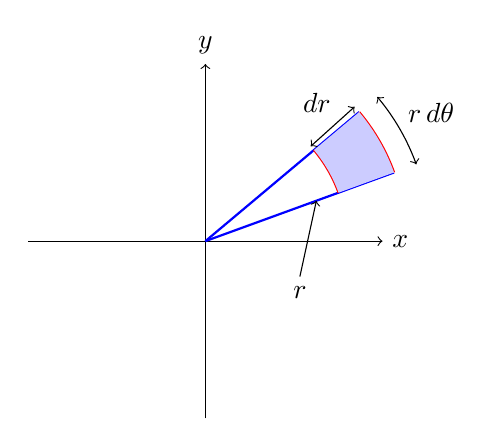
\begin{tikzpicture}[scale=1.5]
    % Draw axes
    \draw[->] (-1.5,0) -- (1.5,0) node[right] {$x$};
    \draw[->] (0,-1.5) -- (0,1.5) node[above] {$y$};
    
    % Draw radial lines
    \draw[blue, thick] (0,0) -- (20:1.7);
    \draw[blue, thick] (0,0) -- (40:1.7);
    
    % Draw arcs
    \draw[red, thick] (20:1.2) arc (20:40:1.2);
    \draw[red, thick] (20:1.7) arc (20:40:1.7);
    
    % Fill area element
    \fill[blue!20] (20:1.2) -- (20:1.7) arc (20:40:1.7) -- (40:1.2) arc (40:20:1.2) -- cycle;
    
    % Labels with manually adjustable positions
    \draw[<->] (42:1.2) -- (42:1.7) node[midway, xshift=-0.2cm, yshift=.3cm] {$dr$};
    \draw[<->] (20:1.9) arc (20:40:1.9) node[midway, xshift=0.4cm, yshift=0.2cm] {$r\,d\theta$};
    
    % Radius label with arrow
    \draw[->] (0.8,-0.3) node[below] {$r$} -- (20:1.0);
\end{tikzpicture}
\caption{\textit{Visualization of a polar area element showing the infinitesimal area $r\,d\theta\,dr$ in polar coordinates.}}
\label{fig:polar_element}
\end{figure}

\noindent At radius $r$, a small angle $d\theta$ creates an arc of length $r\,d\theta$ (just as the circumference of a circle is $2\pi r$). The radial thickness of our element is $dr$. Therefore, our area element is approximately a rectangle with:
\begin{align*}
\text{width} &= r\,d\theta \\
\text{height} &= dr
\end{align*}

\noindent Multiplying these gives our area element:
\[
dA = r\,dr\,d\theta
\]

\noindent This explains why the factor of $r$ appears—as we move farther from the origin (larger $r$), the same angle $d\theta$ sweeps out a longer arc, creating a larger area element. The actual area element becomes exact as $dr$ and $d\theta$ become infinitesimally small. If we also think about the units this also makes sense: Area requires a squared length, and thus $r$ and $dr$ provide the length. $d\theta$ is unitless since it's an angle. \\ \\
\noindent \textbf{Common Mistake:} The most frequent error in polar integration is writing \( dA = dr \, d\theta \) instead of \( dA = r \, dr \, d\theta \). Every polar double integral must include the extra factor of \( r \). Forgetting it will give an answer with wrong units and wrong magnitude.\\ \\

\noindent Therefore once considering the surface function $f(x,y)$ for the height and transforming it to polar: $f(x,y) = f(r\cos\theta,r\sin\theta) = g(r,\theta)$, a double integral in polar coordinates takes the general form:
\[
\iint_R f(x,y)\,dA = \iint_R f(r\cos\theta, r\sin\theta)\,r\,dr\,d\theta =  \iint_R g(r,\theta)\,r\,dr\,d\theta 
\]

\subsubsection*{Setting Up Polar Double Integrals}

\noindent When working with double integrals in polar coordinates, students must follow a systematic approach that transforms the rectangular coordinate integration into a more manageable polar coordinate representation. Let's break down the process step by step:

\begin{enumerate}
   \item \textbf{Identify the Bounds on $r$ and $\theta$:} 
    This crucial first step involves carefully determining the limits of your integration region. Unlike rectangular coordinates where you define rectangular bounds, in polar coordinates you'll specify:
    \begin{itemize}
        \item The range of radial distance $r$ from the origin, which determines how far out you'll integrate
        \item The range of angle $\theta$, which determines the angular sweep of your region
    \end{itemize}
    Think of this as creating a pie slice or full circle in the coordinate plane. The limits will depend on the specific geometric region you're integrating over.

   \item \textbf{Convert the Integrand from Rectangular to Polar Coordinates:}
    This involves replacing rectangular variables with their polar equivalents:
    \begin{align*}
    x &= r\cos\theta \\
    y &= r\sin\theta
    \end{align*}
    Any function $f(x,y)$ becomes $f(r\cos\theta, r\sin\theta)$. For instance, $x^2 + y^2$ simply becomes $r^2$.

   \item \textbf{Include the Factor of $r$ from the Area Element:}
    In polar coordinates, the differential area changes from $dA = dx\,dy$ to $dA = r\,dr\,d\theta$. This critical $r$ factor accounts for the expanding arc length as you move further from the origin. Always multiply your integrand by $r$ to maintain the correct area scaling.

   \item \textbf{Set Up the Integral with the Appropriate Order of Integration:}
    Typically, you'll integrate with respect to $r$ first, then $\theta$. This approach mimics how you'd conceptually sweep radial lines through their angular range, progressively building up the area of your region.
\end{enumerate}

\noindent The natural order of integration in polar coordinates is usually to integrate with respect to $r$ first, then $\theta$. This corresponds to integrating along radial lines from the origin, then sweeping these lines through the required angular range. \\

\noindent Some expressions become particularly simple in polar coordinates:
\begin{itemize}
   \item $x^2 + y^2 = r^2$
   \item $\tan^{-1}(\frac{y}{x}) = \theta$
   \item $\sqrt{x^2 + y^2} = r$
\end{itemize}


\subsubsection*{Standard Regions in Polar Coordinates}

\noindent Several types of standard regions are particularly well-suited to polar coordinates:

\begin{enumerate}
   \item \textbf{Circular Disks:} For a disk of radius $a$:
       \begin{align*}
       0 &\leq r \leq a \\
       0 &\leq \theta \leq 2\pi
       \end{align*}
   
   \item \textbf{Circular Sectors:} For a sector of radius $a$ from angle $\alpha$ to $\beta$:
       \begin{align*}
       0 &\leq r \leq a \\
       \alpha &\leq \theta \leq \beta
       \end{align*}
   
   \item \textbf{Annuli:} For a region between circles of radius $a$ and $b$:
       \begin{align*}
       a &\leq r \leq b \\
       0 &\leq \theta \leq 2\pi
       \end{align*}
\end{enumerate}

\begin{center}
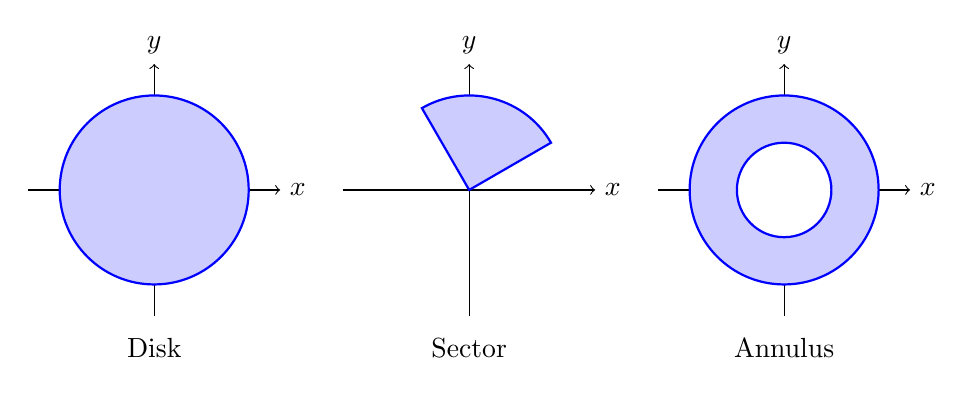
\begin{tikzpicture}[scale=0.8]
   % First subplot - Circle
   \begin{scope}
       % Draw axes
       \draw[->] (-2,0) -- (2,0) node[right] {$x$};
       \draw[->] (0,-2) -- (0,2) node[above] {$y$};
       
       % Draw circle
       \fill[blue!20] (0,0) circle (1.5);
       \draw[blue, thick] (0,0) circle (1.5);
       
       \node[below] at (0,-2.2) {Disk};
   \end{scope}
   
   % Second subplot - Sector
   \begin{scope}[xshift=5cm]
       % Draw axes
       \draw[->] (-2,0) -- (2,0) node[right] {$x$};
       \draw[->] (0,-2) -- (0,2) node[above] {$y$};
       
       % Draw sector
       \fill[blue!20] (0,0) -- (30:1.5) arc (30:120:1.5) -- cycle;
       \draw[blue, thick] (0,0) -- (30:1.5) arc (30:120:1.5) -- cycle;
       
       \node[below] at (0,-2.2) {Sector};
   \end{scope}
   
   % Third subplot - Annulus
   \begin{scope}[xshift=10cm]
       % Draw axes
       \draw[->] (-2,0) -- (2,0) node[right] {$x$};
       \draw[->] (0,-2) -- (0,2) node[above] {$y$};
       
       % Draw annulus
       \fill[blue!20] (0,0) circle (1.5);
       \fill[white] (0,0) circle (0.75);
       \draw[blue, thick] (0,0) circle (1.5);
       \draw[blue, thick] (0,0) circle (0.75);
       
       \node[below] at (0,-2.2) {Annulus};
   \end{scope}
\end{tikzpicture}
\end{center}




\exampleline
\begin{example}
Evaluate the double integral \(\displaystyle\iint_R (x^2 + y^2)\,dA\), where $R$ is the circular disk bounded by $r = 2$.

\begin{solution} This problem is ideal for polar coordinates due to the circular symmetry of the region. Let's solve it step by step:

\noindent First, note the transformation from rectangular to polar coordinates:
\begin{itemize}
    \item $x^2 + y^2 = r^2$
    \item $dA = r\,dr\,d\theta$
\end{itemize}

\noindent For the circular disk, the bounds are straightforward:
\begin{align*}
0 &\leq r \leq 2 \\
0 &\leq \theta \leq 2\pi
\end{align*}

\noindent Transforming the integral:
\begin{align*}
\iint_R (x^2 + y^2)\,dA &= \int_0^{2\pi} \int_0^2 r^2 \cdot r\,dr\,d\theta \\
&= \int_0^{2\pi} \left[\frac{r^4}{4}\right]_0^2 \,d\theta \\
&= 8\pi
\end{align*}

\noindent The final result is $8\pi$, demonstrating how polar coordinates simplify the integration of this radially symmetric function.
\end{solution}
\end{example}
\exampleline

\subsubsection*{Irregular Regions in Polar Coordinates} 


\noindent Now let's think about what happens when we don't have a standard region, but one that is defined by polar functions. Consider the figure below, which shows an irregular region $R$ bounded by two curves in polar form $r = h_1(\theta)$ and $r = h_2(\theta)$. Above this region, a surface $z = f(x,y)$ creates a volume that we might want to calculate. The vertical lines represent the height of the surface at various points, while the polar grid below shows how we divide the region for integration. This is essentially the polar version of the Riemann sum we saw in the previous lecture.

\begin{figure}[H]
\centering
\tdplotsetmaincoords{70}{110}
\begin{tikzpicture}[tdplot_main_coords, line cap=round, >=stealth, scale=1.5,
declare function={
surfacefn(\x,\y)=2.5+0.15*sin(45*\x)+0.15*cos(45*\y);
innerbound(\t)=1+0.2*cos(2*\t);
outerbound(\t)=2.5+0.3*sin(3*\t);
}
]
% Axes with normal-sized labels
\draw[->] (0,0,0) coordinate (O) -- (4,0,0) node[pos=1.05]{$x$};
\draw[->] (O) -- (0,4,0) node[pos=1.05]{$y$};
\draw[->] (O) -- (0,0,4) node[pos=1.05]{$z$};

% Base polar grid
\foreach \r in {0.5,1,...,3} {
\draw[gray!20] ({\r*cos(0)},{\r*sin(0)},0) arc (0:360:\r);
}

% Polar subdivisions
\foreach \t in {0,30,...,330} {
\pgfmathsetmacro{\rTwo}{outerbound(\t)}
\draw[gray!40] (0,0,0) -- ({\rTwo*cos(\t)},{\rTwo*sin(\t)},0);
}

% Surface mesh
\foreach \x in {-3,-2.5,...,3} {
\draw[blue!40,thin,opacity=0.4] plot[variable=\y,domain=-3:3,samples=30]
(\x,\y,{surfacefn(\x,\y)});
}
\foreach \y in {-3,-2.5,...,3} {
\draw[blue!40,thin,opacity=0.4] plot[variable=\x,domain=-3:3,samples=30]
(\x,\y,{surfacefn(\x,\y)});
}

% Fill surface
\foreach \x in {-3,-2.5,...,2.5} {
\foreach \y in {-3,-2.5,...,2.5} {
\pgfmathsetmacro{\nextx}{\x+0.5}
\pgfmathsetmacro{\nexty}{\y+0.5}
\pgfmathsetmacro{\z}{surfacefn(\x,\y)}
\fill[blue!30,opacity=0.6]
(\x,\y,\z) --
(\nextx,\y,{surfacefn(\nextx,\y)}) --
(\nextx,\nexty,{surfacefn(\nextx,\nexty)}) --
(\x,\nexty,{surfacefn(\x,\nexty)}) -- cycle;
}
}

% Projection of region on surface
\draw[gray!40, fill=gray!20, opacity=0.8]
plot[variable=\t,domain=0:360,samples=120]
({innerbound(\t)*cos(\t)},{innerbound(\t)*sin(\t)},{surfacefn(innerbound(\t)*cos(\t),innerbound(\t)*sin(\t))})
plot[variable=\t,domain=360:0,samples=120]
({outerbound(\t)*cos(\t)},{outerbound(\t)*sin(\t)},{surfacefn(outerbound(\t)*cos(\t),outerbound(\t)*sin(\t))});

% Volume element edges
\foreach \t in {0,30,...,330} {
\pgfmathsetmacro{\rOne}{innerbound(\t)}
\pgfmathsetmacro{\rTwo}{outerbound(\t)}
\pgfmathsetmacro{\xOne}{\rOne*cos(\t)}
\pgfmathsetmacro{\yOne}{\rOne*sin(\t)}
\pgfmathsetmacro{\xTwo}{\rTwo*cos(\t)}
\pgfmathsetmacro{\yTwo}{\rTwo*sin(\t)}

\draw[gray, dotted, thick]
(\xOne,\yOne,0) -- (\xOne,\yOne,{surfacefn(\xOne,\yOne)});
\draw[gray, dotted, thick]
(\xTwo,\yTwo,0) -- (\xTwo,\yTwo,{surfacefn(\xTwo,\yTwo)});
}

% Boundary curves with labels
\draw[red,thick] plot[variable=\t,domain=0:360,samples=120]
({outerbound(\t)*cos(\t)},{outerbound(\t)*sin(\t)},0);
\draw[blue,thick] plot[variable=\t,domain=0:360,samples=120]
({innerbound(\t)*cos(\t)},{innerbound(\t)*sin(\t)},0);

% Adding labels for h₁(θ) and h₂(θ)
\node[blue] at (1.3,0.9,0) {$h_1(\theta)$};
\node[red] at (2.9,1.9,0) {$h_2(\theta)$};

\end{tikzpicture}
\caption{\textit{Volume integral in polar coordinates with a gently undulating surface.}}
\end{figure}




\noindent Now the next figure provides a detailed view of how we construct our polar integral for our irregular region. We focus on a section of the first quadrant (from $\pi/6$ to $\pi/3$) to see the structure more clearly. The highlighted area element demonstrates how $dr$ represents the radial thickness while $r\,d\theta$ gives the arc length at radius $r$. Notice that this wedge-shaped element grows wider as $r$ increases—this growth is precisely what the factor of $r$ in our area element accounts for.


\begin{figure}[H]
\centering
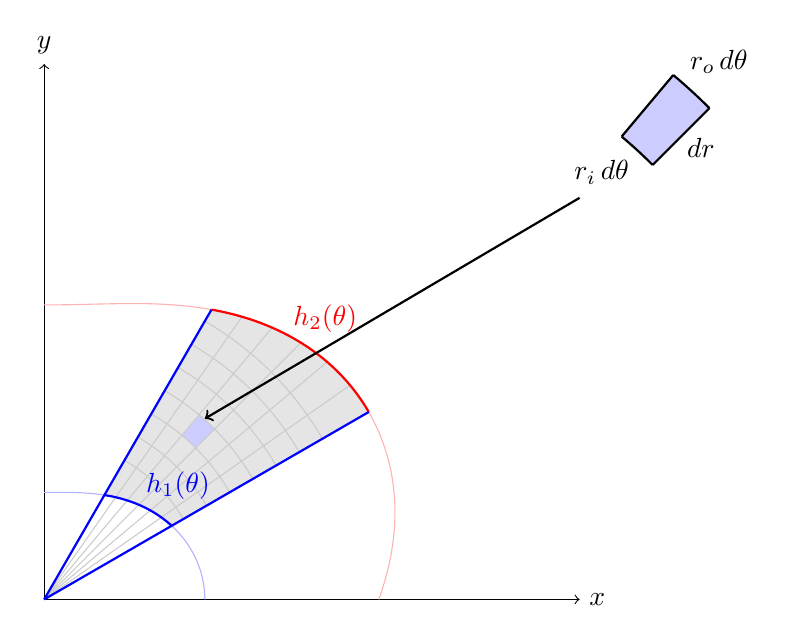
\begin{tikzpicture}[scale=1.7,
declare function={
h1(\t)=1+0.2*cos(2*\t);
h2(\t)=2.5+0.3*sin(3*\t);
}]
% Draw axes
\draw[->] (0,0) -- (4,0) node[right] {$x$};
\draw[->] (0,0) -- (0,4) node[above] {$y$};

% Draw the curved boundaries for first quadrant section (full section for context)
\draw[blue!30, thin] plot[variable=\t, domain=0:90, samples=100]
({h1(\t)*cos(\t)}, {h1(\t)*sin(\t)});
\draw[red!30, thin] plot[variable=\t, domain=0:90, samples=100]
({h2(\t)*cos(\t)}, {h2(\t)*sin(\t)});

% Draw and fill the middle third (π/6 to π/3)
\fill[gray!20] plot[variable=\t, domain=30:60, samples=100]
({h1(\t)*cos(\t)}, {h1(\t)*sin(\t)})
-- plot[variable=\t, domain=60:30, samples=100]
({h2(\t)*cos(\t)}, {h2(\t)*sin(\t)}) -- cycle;

% Fill a specific grid cell in the middle to highlight it
\fill[blue!20] (45:1.6) arc (45:50:1.6) -- (50:1.8) arc (50:45:1.8) -- cycle;

% Add circular grid lines clipped between h1 and h2
\begin{scope}
% Define the clipping path to the middle third region between h1 and h2
\clip plot[variable=\t, domain=30:60, samples=100]
({h1(\t)*cos(\t)}, {h1(\t)*sin(\t)})
-- plot[variable=\t, domain=60:30, samples=100]
({h2(\t)*cos(\t)}, {h2(\t)*sin(\t)}) -- cycle;

% Draw the circular grid lines within the clipped region
\foreach \r in {1.2,1.4,...,2.4} {
\draw[gray!40] (30:\r) arc (30:60:\r);
}
\end{scope}

% Draw the angular grid lines from origin to h2
\foreach \t in {35,40,...,55} {
\pgfmathsetmacro{\rmax}{h2(\t)}
\draw[gray!40] (0,0) -- (\t:\rmax);
}

% Draw the boundaries of the middle third more prominently
\draw[blue, thick] plot[variable=\t, domain=30:60, samples=100]
({h1(\t)*cos(\t)}, {h1(\t)*sin(\t)});
\draw[red, thick] plot[variable=\t, domain=30:60, samples=100]
({h2(\t)*cos(\t)}, {h2(\t)*sin(\t)});

% Draw the bounding radial lines
\pgfmathsetmacro{\rmaxStart}{h2(30)}
\pgfmathsetmacro{\rmaxEnd}{h2(60)}
\draw[blue, thick] (0,0) -- (30:\rmaxStart);
\draw[blue, thick] (0,0) -- (60:\rmaxEnd);

% Add arrow pointing to the highlighted cell
\draw[->, thick] (4,3) -- (1.2,1.35);

% Add labels for h₁(θ) and h₂(θ)
\node[blue] at (1,0.85) {$h_1(\theta)$};
\node[red] at (2.1,2.1) {$h_2(\theta)$};

\begin{scope}[shift={(2,0.7)}, scale=3]
% Draw the curved quasi-rectangular element
\fill[blue!20] (45:1.2) arc (45:50:1.2) -- (50:1.4) arc (50:45:1.4) -- cycle;

% Draw the boundary lines
\draw[thick] (45:1.2) arc (45:50:1.2); % Inner arc
\draw[thick] (45:1.4) arc (45:50:1.4); % Outer arc
\draw[thick] (45:1.2) -- (45:1.4); % Left radial line
\draw[thick] (50:1.2) -- (50:1.4); % Right radial line

% Labels with adjustable positions using xshift and yshift
\node[xshift=0.8cm, yshift=-0.3cm] at (49.5:1.25) {$dr$};
\node[xshift=0cm, yshift=0cm] at (49:1.1) {$r_i\,d\theta$};
\node[xshift=0cm, yshift=0cm] at (47.5:1.5) {$r_o\,d\theta$};
\end{scope}

\end{tikzpicture}
\caption{\textit{Middle third section ($\pi/6$ to $\pi/3$) of the polar region with grid lines and detailed view of infinitesimal area element.}}
\label{fig:polar_region_detail}
\end{figure}

\noindent Let's see how to mathematically construct the integral for this example now. Given a region $R$ bounded by two curves $r = h_1(\theta)$ and $r = h_2(\theta)$, with $h_1(\theta) \leq h_2(\theta)$, our general integral takes the form:

\[
\iint_R f(x,y)\,dA = \int_{\alpha}^{\beta} \int_{h_1(\theta)}^{h_2(\theta)} f(r\cos\theta, r\sin\theta)\,r\,dr\,d\theta
\]

\noindent where:
\begin{itemize}
   \item $[\alpha,\beta]$ represents the angular range of the region. In the case of the whole region in this example we would have $\alpha = 0$, $\beta = 2\pi$.
   \item $h_1(\theta)$ gives the inner boundary curve
   \item $h_2(\theta)$ gives the outer boundary curve
   \item The factor $r$ appears from our area element $dA = r\,dr\,d\theta$
\end{itemize}

\noindent Just as with rectangular coordinates, we integrate from the inner bound to the outer bound, but now these bounds are functions of our angular variable $\theta$. The key difference is that we must include the factor of $r$ from our area element, which accounts for the expanding size of our wedge-shaped regions as we move outward from the origin.

\exampleline
\begin{example}
An engineering team is excavating a basin in the first quadrant as shown below. The basin is bounded by two circular arcs whose centers are marked in the diagram. Each point in the basin has a depth proportional to the angle it makes with the positive x-axis, given by
\[
z = \arctan\!\Bigl(\tfrac{y - \frac{1}{2}}{x- \frac{1}{2}}\Bigr).
\]
Using the diagram information, determine the total volume of soil to be removed.

\begin{figure}[H]
\centering
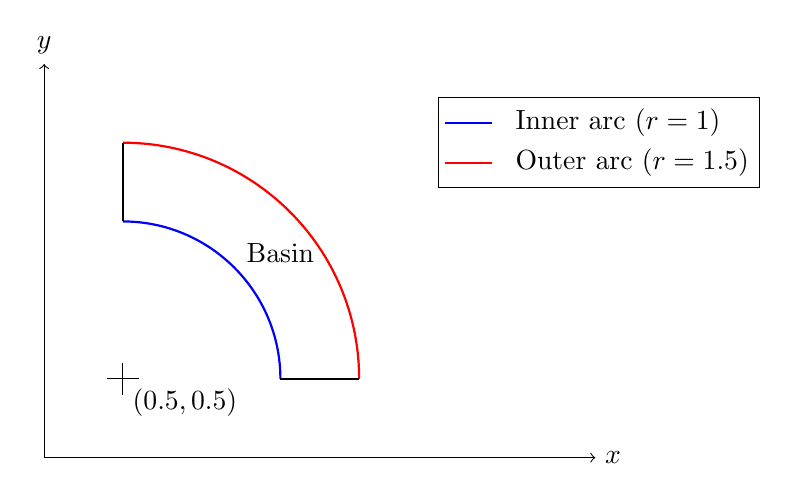
\begin{tikzpicture}[scale=2]
% Axes
\draw[->] (0,0) -- (3.5,0) node[right] {$x$};
\draw[->] (0,0) -- (0,2.5) node[above] {$y$};

% Define center and radii
\def\centerX{0.5}
\def\centerY{0.5}
\def\innerRadius{1}
\def\outerRadius{1.5}

% Inner circle arc
\draw[blue, thick] (\centerX,\centerY) ++(0:\innerRadius) arc (0:90:\innerRadius);

% Outer circle arc
\draw[red, thick] (\centerX,\centerY) ++(0:\outerRadius) arc (0:90:\outerRadius);

% Boundary lines between the arcs
\draw[black, thick] (\centerX+\innerRadius,\centerY) -- (\centerX+\outerRadius,\centerY);
\draw[black, thick] (\centerX,\centerY+\innerRadius) -- (\centerX,\centerY+\outerRadius);

% Center marker (crosshair)
\draw[black, thin] (\centerX-0.1,\centerY) -- (\centerX+0.1,\centerY);
\draw[black, thin] (\centerX,\centerY-0.1) -- (\centerX,\centerY+0.1);

% Center point label
\node[below right] at (\centerX,\centerY) {$(0.5,0.5)$};

% Basin label
\node at (1.5,1.3) {Basin};



% Matrix-style legend
\matrix [draw=black, fill=white, inner sep=0.2em, row sep=0.05em, column sep=0.6em,
anchor=west] at (2.5,2)
{
\draw[blue, thick] (0,0) -- (0.6,0); & \node[align=left] {Inner arc ($r=1$)}; \\
\draw[red, thick] (0,0) -- (0.6,0); & \node[align=left] {Outer arc ($r=1.5$)}; \\
};

\end{tikzpicture}
\end{figure}

\begin{solution}
Let's solve this step by step:

\begin{enumerate}
\item Analyze the region from the diagram. The basin consists of points $(x,y)$ in the first quadrant where the distance from $(0.5, 0.5)$ is between $1$ and $1.5$. If we let $r$ be that distance and $\theta$ the angle measured from the positive $x$-axis (through the center $(0.5, 0.5)$), then:
\[
r = \sqrt{(x - 0.5)^2 + (y - 0.5)^2}, 
\quad
\tan(\theta) = \frac{y - 0.5}{x - 0.5}.
\]
The basin boundaries give us:
\[
0 \leq \theta \leq \frac{\pi}{2}
\quad\text{and}\quad
1 \leq r \leq 1.5.
\]

\item Simplify the height function. Inside the arctan, we have:
\[
\frac{y - 0.5}{x - 0.5}
= \frac{r \sin(\theta)}{r \cos(\theta)}
= \tan(\theta).
\]
Therefore:
\[
z = \arctan(\tan(\theta)) = \theta
\quad
\text{since }0\leq \theta \leq \frac{\pi}{2}.
\]

\item Set up and evaluate the volume integral. Using polar coordinates centered at $(0.5,0.5)$, the differential area element is $r\,dr\,d\theta$. The volume is:
\[
\text{Volume} = \iint_{\text{basin}} z \, dA 
= \int_{0}^{\pi/2} \int_{1}^{1.5} \theta \,r \,dr\,d\theta.
\]

First, integrate with respect to $r$:
\begin{align*}
\int_{1}^{1.5} \theta \,r \,dr 
&= \theta \int_{1}^{1.5} r \,dr \\
&= \theta \left[\frac{r^2}{2}\right]_{r=1}^{r=1.5} \\
&= \theta\left(\frac{(1.5)^2}{2} - \frac{1^2}{2}\right) \\
&= \theta(1.125 - 0.5) \\
&= 0.625\theta.
\end{align*}

Now integrate with respect to $\theta$:
\begin{align*}
\int_{0}^{\pi/2} 0.625\theta \,d\theta 
&= 0.625 \int_{0}^{\pi/2} \theta \,d\theta \\
&= 0.625 \left[\frac{\theta^2}{2}\right]_{0}^{\pi/2} \\
&= 0.625 \cdot \frac{(\pi/2)^2}{2} \\
&= \frac{5\pi^2}{64}.
\end{align*}
\end{enumerate}

Therefore, the volume of soil to be removed is $\frac{5\pi^2}{64}$ cubic units.
\end{solution}


\end{example}


\exampleline
\begin{example}
Find the value of the integral
\[
\int_{-\infty}^{\infty} e^{-x^2} \,dx.
\]
\begin{solution}
\begin{enumerate}
\item Let \( I = \int_{-\infty}^{\infty} e^{-x^2} \,dx \).

\item Square it:
\[
I^2 = \left(\int_{-\infty}^{\infty} e^{-x^2} \,dx\right)
      \left(\int_{-\infty}^{\infty} e^{-y^2} \,dy\right)
    = \int_{-\infty}^{\infty}\int_{-\infty}^{\infty} e^{-(x^2 + y^2)} \,dx\,dy.
\]

\item Switch to polar coordinates with \( x = r\cos\theta,\; y = r\sin\theta \). The change in variable to polar coordinates gives \( dx\,dy = r\,dr\,d\theta \). The bounds are \( r:0\to\infty \) and \( \theta:0\to 2\pi \):
\[
I^2 = \int_{0}^{2\pi} \int_{0}^{\infty} e^{-r^2} r \,dr\,d\theta.
\]

\item Separate the integrals:
\[
I^2 = \left(\int_{0}^{2\pi} d\theta\right)
      \left(\int_{0}^{\infty} e^{-r^2} r \,dr\right)
    = 2\pi \int_{0}^{\infty} e^{-r^2} r \,dr.
\]

\item Use the substitution \( u = r^2 \), so \( du = 2r\,dr \) and \( r\,dr = \tfrac12\,du \):
\[
I^2 = 2\pi \int_{0}^{\infty} e^{-r^2} r \,dr
    = 2\pi \int_{0}^{\infty} e^{-u} \,\frac12\,du
    = \pi \int_{0}^{\infty} e^{-u}\,du 
    = \pi \left[-e^{-u}\right]_{0}^{\infty} 
    = \pi \cdot 1 
    = \pi.
\]

\item Hence \( I = \sqrt{\pi} \). Therefore,
\[
\int_{-\infty}^{\infty} e^{-x^2} \,dx = \sqrt{\pi}.
\]
\noindent This is a common technique used to integrate functions with impossible anti-derivatives.
\end{enumerate}

\end{solution}
\end{example}
\exampleline


\subsubsection*{Complex Regions and Multiple Integrals}

\noindent Not all regions can be neatly categorized as Type I or Type II. Consider a region bounded by multiple curves where vertical or horizontal lines might intersect the boundary more than twice. In such cases, we must break down our region into simpler pieces where our integration techniques apply. \\

\noindent The fundamental principle we use is the additivity of integrals:
\[
\iint_R f(x,y) \,dA = \iint_{R_1} f(x,y) \,dA + \iint_{R_2} f(x,y) \,dA
\]
where $R = R_1 \cup R_2$ and $R_1 \cap R_2 = \emptyset$ \\

\noindent Consider, for example, the region bounded by $y = x^2$ and $y = 4$:

\begin{figure}[H]
\begin{center}
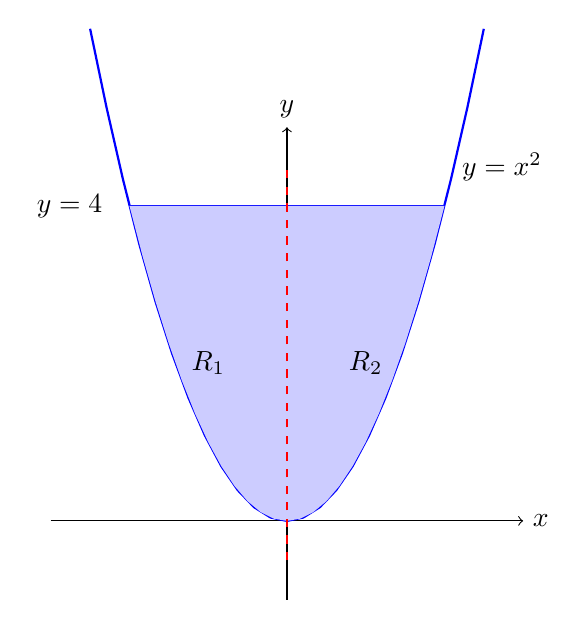
\begin{tikzpicture}[scale=1]
    % Draw axes
    \draw[->] (-3,0) -- (3,0) node[right] {$x$};
    \draw[->] (0,-1) -- (0,5) node[above] {$y$};
    
    % Draw curves
    \draw[blue, thick, domain=-2.5:2.5] plot (\x, {\x*\x});
    \draw[blue, thick] (-2,4) -- (2,4);
    
    % Fill regions
    \fill[blue!20] plot[domain=-2:2] (\x, {\x*\x}) -- (2,4) -- (-2,4) -- cycle;
    
    % Draw vertical lines showing division
    \draw[red, dashed] (0,-0.5) -- (0,4.5);
    
    % Label regions
    \node at (-1,2) {$R_1$};
    \node at (1,2) {$R_2$};
    
    % Label curves
    \node[right] at (-3.3,4) {$y = 4$};
    \node[right] at (2.1,4.5) {$y = x^2$};
\end{tikzpicture}
\end{center}
\caption{\textit{A parabola that can be split into two regions due to additivity of integrals.}}
\end{figure}

\noindent This region can be split into two Type I regions at $x = 0$:

\begin{itemize}
    \item $R_1$: Region where $-2 \leq x \leq 0$, $x^2 \leq y \leq 4$
    \item $R_2$: Region where $0 \leq x \leq 2$, $x^2 \leq y \leq 4$
\end{itemize}

\noindent Sometimes a region might be better described by splitting it into Type II regions:

\begin{figure}[H]
\begin{center}
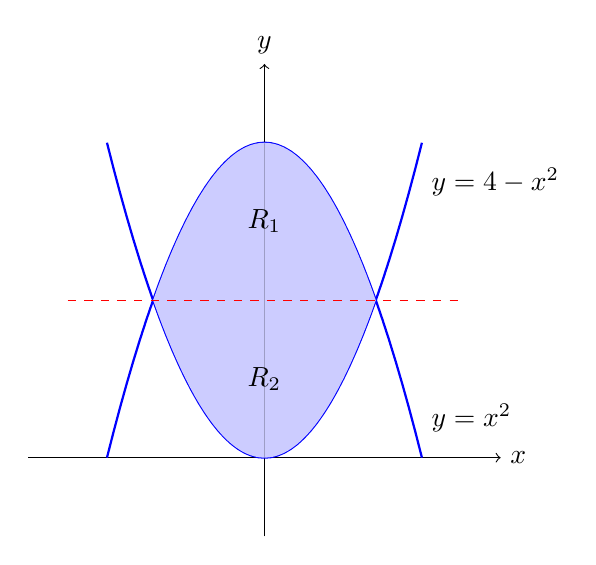
\begin{tikzpicture}[scale=1]
% Draw axes
\draw[->] (-3,0) -- (3,0) node[right] {$x$};
\draw[->] (0,-1) -- (0,5) node[above] {$y$};

% Draw curves
\draw[blue, thick, domain=0:2] plot (\x, {4-\x*\x});
\draw[blue, thick, domain=0:2] plot (\x, {\x*\x});
\draw[blue, thick, domain=0:2] plot (-\x, {4-\x*\x});
\draw[blue, thick, domain=0:2] plot (-\x, {\x*\x});

% Fill regions only between -√2 and √2
\fill[blue!20] plot[domain=0:1.4142] (\x, {4-\x*\x}) -- plot[domain=1.4142:0] (\x, {\x*\x});
\fill[blue!20] plot[domain=0:1.4142] (-\x, {4-\x*\x}) -- plot[domain=1.4142:0] (-\x, {\x*\x});

% Draw horizontal line showing division
\draw[red, dashed] (-2.5,2) -- (2.5,2);

% Label regions
\node at (0,3) {$R_1$};
\node at (0,1) {$R_2$};

% Label curves
\node[right] at (2,0.5) {$y = x^2$};
\node[right] at (2,3.5) {$y = 4-x^2$};
\end{tikzpicture}
\end{center}
\caption{\textit{An otherwise Type I region that is converted into Type II by adjusting the equations and finding the appropriate intersection point.}}
\end{figure}

\noindent Here, we might split at $y = 2$ into:
\begin{itemize}
    \item $R_1$: Region where $2 \leq y \leq 4$, $-\sqrt{4-y} \leq x \leq \sqrt{4-y}$
    \item $R_2$: Region where $0 \leq y \leq 2$, $-\sqrt{y} \leq x \leq \sqrt{y}$
\end{itemize}

\noindent When working with complex regions, we often encounter situations that require more sophisticated splitting strategies:

\begin{figure}[H]
\centering
\begin{center}
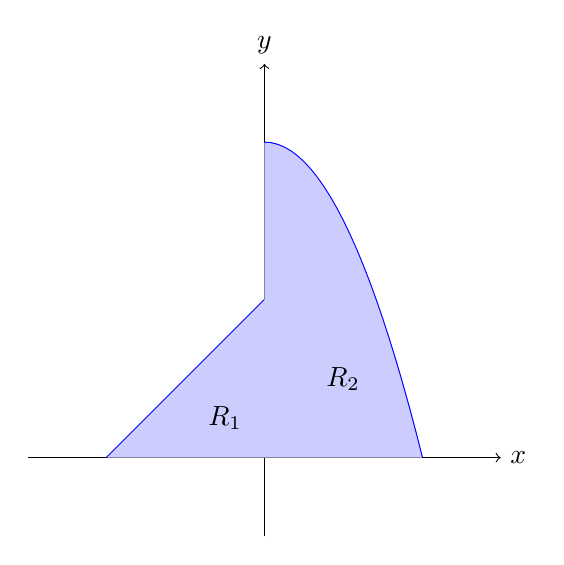
\begin{tikzpicture}[scale=1]
    % Draw axes
    \draw[->] (-3,0) -- (3,0) node[right] {$x$};
    \draw[->] (0,-1) -- (0,5) node[above] {$y$};
    
    % Draw curves - piecewise example
    \draw[blue, thick] (-2,0) -- (0,2);
    \draw[blue, thick, domain=0:2] plot (\x, {4-\x*\x});
    
    % Fill region
    \fill[blue!20] (-2,0) -- (0,2) -- plot[domain=0:2] (\x, {4-\x*\x}) -- (2,0) -- cycle;
    
    % Label regions
    \node at (-.5,.5) {$R_1$};
    \node at (1,1) {$R_2$};
    
\end{tikzpicture}
\end{center}
\caption{\textit{Two piece-wise defined Type I regions.}}
\end{figure}

\noindent For piecewise-defined regions, natural splitting points occur where the boundary function changes form. Each piece may suggest a different integration approach—Type I or Type II—based on the function's behavior. \\

\noindent Some regions may benefit from mixing coordinate systems. Consider the region bounded by $y = x^2$ and $r = 2$:

\begin{figure}[H]
\begin{center}
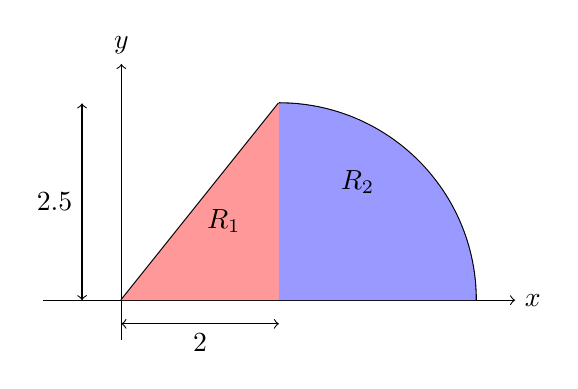
\begin{tikzpicture}[scale=1]
    % Draw axes
    \draw[->] (-1,0) -- (5,0) node[right] {$x$};
    \draw[->] (0,-0.5) -- (0,3) node[above] {$y$};
    
    % Constants for height and width
    \def\h{2.5} % height of triangle/radius of circle
    
    % Draw boundaries
    \draw[thick] (0,0) -- (2,\h); % Left line of triangle
    \draw[thick] (2,0) -- (2,\h); % Vertical line
    \draw[thick] (2,\h) arc (90:0:2.5); % Quarter circle
    
    % Fill regions
    \fill[red!40] (0,0) -- (2,\h) -- (2,0) -- cycle; % R1 (triangle)
    \fill[blue!40] (2,0) -- (2,\h) arc (90:0:2.5) -- (4.5,0) -- cycle; % R2 (quarter circle)
    
    % Label regions
    \node at (1.3,1) {$R_1$};
    \node at (3,1.5) {$R_2$};
    
    % Add dimension labels
    \draw[<->] (-0.5,0) -- (-0.5,\h) node[midway,left] {$2.5$};
    \draw[<->] (0,-0.3) -- (2,-0.3) node[midway,below] {$2$};

\end{tikzpicture}
\end{center}
\caption{\textit{Two piece-wise defined regions where $R_1$ and $R_2$ can be the bounds of two double integrals with different coordinate systems. The height of the triangle and radius of the quarter circle are both 2.5 units.}}
\label{fig:doubleregion}
\end{figure}

\noindent Here, the left region $R_1$ might be better described using Cartesian coordinates, while the right region $R_2$ could be more naturally integrated using polar coordinates to handle the circular boundary. When determining how to split a region:
\begin{itemize}
    \item Consider the form of both the boundary curves and the integrand
    \item Look for symmetry that could simplify calculations
    \item Evaluate whether changing coordinate systems might simplify the integration
    \item Balance the number of subregions against the complexity of individual integrals
\end{itemize}

\exampleline
\begin{example}
\begin{enumerate}
\item Find the area of the region shown in Figure \ref{fig:doubleregion} by evaluating the double integral
\[
\iint_{R = R_1 \cup R_2} dA
\]
\item Use the surface $f(x,y) = x^2 + y^2 + 1$ to find the volume over the region $R$.
\end{enumerate}

\begin{solution}
\begin{enumerate}
\item For finding the area:
\begin{enumerate}

\item First, we split the integral using the additivity property:
\[
\iint_R dA = \iint_{R_1} dA + \iint_{R_2} dA
\]

\item For region $R_1$, we can use Cartesian coordinates. The region is a triangle bounded by $x=0$, $x=2$, and the line passing through $(0,0)$ and $(2,2.5)$. The equation of this line is $y = \frac{5}{4}x$:
\[
\iint_{R_1} dA = \int_0^2 \int_0^{\frac{5}{4}x} dy\,dx = \int_0^2 \frac{5}{4}x\,dx = \frac{5}{2}
\]

\item For region $R_2$, we can use polar coordinates since it's a quarter circle of radius 2.5 centered at $(2,0)$. We need to shift our polar coordinates by translating 2 units right:
\[
\iint_{R_2} dA = \int_0^{\pi/2} \int_0^{2.5} r\,dr\,d\theta = \frac{\pi}{4}(2.5)^2
\]

\item The total area is therefore:
\[
\text{Area} = \frac{5}{2} + \frac{25\pi}{16} \approx 7.42 \text{ square units}
\]


\end{enumerate}

\item Now for our surface function $f(x,y)$, we would have to integrate $f(x,y)$ over $R_1$, and then have to integrate $f(r\cos\theta,r\sin\theta) = g(r,\theta)$ over $R_2$.
\begin{enumerate}
\item For integrating $f(x,y) = x^2 + y^2 + 1$ over $R_1$, we use Cartesian coordinates:
\[
\iint_{R_1} f(x,y)\,dA = \int_0^2 \int_0^{\frac{5}{4}x} (x^2 + y^2 + 1)\,dy\,dx
\]
Evaluating the inner integral:
\[
\int_0^2 \left[x^2y + \frac{y^3}{3} + y\right]_0^{\frac{5}{4}x}\,dx
= \int_0^2 \left(x^2(\frac{5}{4}x) + \frac{1}{3}(\frac{5}{4}x)^3 + \frac{5}{4}x\right)\,dx
\]
\[
= \int_0^2 \left(\frac{5}{4}x^3 + \frac{125}{192}x^3 + \frac{5}{4}x\right)\,dx
= \left[\frac{5}{16}x^4 + \frac{125}{768}x^4 + \frac{5}{8}x^2\right]_0^2
\]
\[
= \frac{5}{16}(16) + \frac{125}{768}(16) + \frac{5}{8}(4) = \frac{485}{48} \approx 10.104
\]

\item For $R_2$, we translate to the center of the quarter circle at $(2,0)$. Using \emph{shifted} polar coordinates centered at $(2,0)$:
\[
x = 2 + r\cos\theta, \quad y = r\sin\theta
\]
\textbf{Note:} Because the polar coordinates are centered at $(2,0)$ and not at the origin, we must substitute carefully into the integrand:
\[
x^2 + y^2 + 1 = (2+r\cos\theta)^2 + r^2\sin^2\theta + 1 = r^2 + 4r\cos\theta + 5.
\]
The integral becomes:
\[
\iint_{R_2} f(x,y)\,dA = \int_0^{\pi/2} \int_0^{2.5} (r^2 + 4r\cos\theta + 5)\,r\,dr\,d\theta
\]
\[
= \int_0^{\pi/2} \int_0^{2.5} (r^3 + 4r^2\cos\theta + 5r)\,dr\,d\theta
\]
\[
= \int_0^{\pi/2} \left[\frac{r^4}{4} + \frac{4r^3}{3}\cos\theta + \frac{5r^2}{2}\right]_0^{2.5}\,d\theta
\]
\[
= \int_0^{\pi/2} \left(\frac{(2.5)^4}{4} + \frac{4(2.5)^3}{3}\cos\theta + \frac{5(2.5)^2}{2}\right)\,d\theta
= \int_0^{\pi/2} \left(9.766 + 20.833\cos\theta + 15.625\right)\,d\theta
\]
\[
= \int_0^{\pi/2} \left(25.391 + 20.833\cos\theta\right)\,d\theta
= \left[25.391\,\theta + 20.833\sin\theta\right]_0^{\pi/2}
\]
\[
= 25.391 \cdot \frac{\pi}{2} + 20.833 \cdot 1 \approx 39.87 + 20.83 = 60.70
\]

\item The total volume is therefore:
\[
V \approx 10.104 + 60.70 = 70.80
\]
\end{enumerate}
\end{enumerate}
\end{solution}
\end{example}
\exampleline



\newpage

\lecture{Applications of Double Integrals}

\noindent In the previous two lectures, we developed the machinery for computing double integrals over rectangular and general regions. We now ask: what physical quantities can these integrals represent? It turns out that mass, balance, rotational resistance, and surface geometry are all naturally expressed as double integrals with the right integrand.\\ \\

\noindent Having established our foundation with area and volume calculations, we now venture into how double integrals illuminate the physical properties of objects in the real world. These applications reveal the deep connection between calculus and physics, showing how mathematical tools can predict and explain the behavior of physical systems.

\subsection*{Mass and Density} \index{Mass and Density}

\noindent When engineers design aircraft wings, solar panels, or electronic circuit boards, they often work with objects that are effectively two-dimensional—their thickness is negligible compared to their other dimensions. For these thin objects, we describe their mass distribution using a density function $\rho(x,y)$ that gives the mass per unit area at each point. This density might vary across the object; think of a solar panel with different components or a circuit board with varying concentrations of conducting material. \\

\noindent To find the total mass of such an object, we integrate the density over the region it occupies:
\[
M = \iint_R \rho(x,y)\,dA
\]

\noindent This integral emerges naturally from the physical principle of additivity of mass—the total mass is the sum of the masses of all small pieces. Each infinitesimal piece has area $dA$ and density $\rho(x,y)$, giving it a mass of $\rho(x,y)\,dA$. The double integral then sums these contributions over the entire region (thus bringing us to the required $M = \rho A_R$ for our units). \\

\noindent Consider, for instance, a sheet of metal that has been treated with a protective coating. The coating might be applied more thickly around the edges, creating a density function that increases as we move away from the center. Or think about a decorative stained glass window, where different colored pieces have different densities. In these cases, the density function captures the physical reality of how mass is distributed across the object.

\subsection*{Center of Mass and Balance} \index{Center of Mass}

\noindent Now that we understand how to represent mass distribution using double integrals, we can tackle an important related problem: finding where an object will balance. Given a flat plate with varying density, where should we place a support to keep it perfectly level? This question leads us to the concept of center of mass. \\

\noindent The center of mass is the balance point of a plate: the location where you could support it on a pin and it would not tip. To find it, we use the principle that the total torque about the balance point must be zero. For a small piece of mass \( dm = \rho(x,y) \, dA \) at position \( (x, y) \), its torque about the \( y \)-axis is \( x \, dm \). Setting the total torque to zero and dividing by the total mass gives:\\ \\

\noindent The center of mass of an object tells us where it effectively balances, a concept crucial in everything from architectural design to spacecraft engineering. For a flat object with density $\rho(x,y)$, we call the coordinates of its center of mass $(\bar{x}, \bar{y})$, given by:
\begin{align*}
\bar{x} &= \frac{1}{M}\iint_R x\rho(x,y)\,dA \\
\bar{y} &= \frac{1}{M}\iint_R y\rho(x,y)\,dA
\end{align*}

\noindent These formulas arise from a fundamental physical principle: the total turning effect (called torque) on an object balanced at its center of mass must be zero. Torque measures the tendency of a force to rotate an object around a point - think of pushing a door near its hinges versus near its handle. Each point in the object creates a torque that depends on both its mass and its distance from the axis. The numerator integrals sum up these effects, while division by the total mass $M$ gives us the balancing point.

%https://tikz.net/dynamics_center_of_mass/          by Izaak Neutelings
% CENTER OF MASS 2D
\begin{figure}[H]
\centering
\begin{tikzpicture} [scale=1.7]
  \def\xmax{4.7} % max x axis
  \def\ymax{3.6} % max y axis
  \coordinate (O) at (0,0);
  \coordinate (M1) at (0.25*\xmax, 0.80*\ymax);
  \coordinate (M2) at (0.38*\xmax, 0.48*\ymax);
  \coordinate (M3) at (0.80*\xmax, 0.20*\ymax);
  \coordinate (M4) at (0.40*\xmax,-0.1*\ymax);
  \coordinate (CM) at (0.50*\xmax, 0.4*\ymax);

  % Axes
  \draw[->,thick] (0,-0.2*\ymax) -- (0,\ymax) node[left] {$y$};
  \draw[->,thick] (-0.2*\xmax,0) -- (\xmax,0) node[below] {$x$};

  % Masses with labels
  \draw[thick,red!60,fill=red!30] (M1) circle(0.12);
  \node[transform shape=false] at ($(M1) + (0.2,0.2)$) {$m_1$}; % Manually adjust here
  \draw[thick,red!60,fill=red!30] (M2) circle(0.10);
  \node[transform shape=false] at ($(M2) + (-0,+0.2)$) {$m_2$}; % Manually adjust here
  \draw[thick,red!60,fill=red!30] (M3) circle(0.14);
  \node[transform shape=false] at ($(M3) + (0.3,-0.2)$) {$m_3$}; % Manually adjust here
  \draw[thick,red!60,fill=red!30] (M4) circle(0.08);
  \node[transform shape=false] at ($(M4) + (-0.2,-0.2)$) {$m_4$}; % Manually adjust here

  % Center of mass with label
  \fill[red!80] (CM) circle(0.08);
  \node[transform shape=false] at ($(CM) + (0.3,0.3)$) {CM}; % Manually adjust here

  % Vectors with labels
  \draw[->,blue!70!black,thick] (O) -- (M1);
  \node[transform shape=false] at ($(O)!0.5!(M1) + (-0.2,0.2)$) {$\vb{r}_1$}; % Manually adjust here
  \draw[->,blue!70!black,thick] (O) -- (M2);
  \node[transform shape=false] at ($(O)!0.5!(M2) + (0.1,0.3)$) {$\vb{r}_2$}; % Manually adjust here
  \draw[->,blue!70!black,thick] (O) -- (M3);
  \node[transform shape=false] at ($(O)!0.5!(M3) + (0.3,-0.15)$) {$\vb{r}_3$}; % Manually adjust here
  \draw[->,blue!70!black,thick] (O) -- (M4);
  \node[transform shape=false] at ($(O)!0.5!(M4) + (-0.3,-0.3)$) {$\vb{r}_4$}; % Manually adjust here
  \draw[->,red!70!black,thick] (O) -- (CM);
  \node[transform shape=false] at ($(O)!0.5!(CM) + (0.3,0.35)$) {$\vb{r}_\mathrm{cm}$}; % Manually adjust here
\end{tikzpicture}
\caption{\textit{A 2D representation of the center of mass (CM) for a system of four masses. The position vectors $\vb{r}_1$, $\vb{r}_2$, $\vb{r}_3$, and $\vb{r}_4$ point from the origin to their respective masses $m_1$, $m_2$, $m_3$, and $m_4$. The center of mass vector $\vb{r}_\mathrm{cm}$ is shown in red, indicating the weighted average position of the masses.}}

\end{figure}

\noindent The practical implications are profound. When aerospace engineers design control surfaces for aircraft, they must carefully consider the center of mass. A poorly balanced aileron or rudder could lead to control issues or mechanical failure. Similarly, architects designing large suspended sculptures must understand exactly where each piece will balance. The center of mass calculations tell them where to place support structures and how to distribute the weight of the artwork. These calculations have real consequences---an incorrectly balanced control surface can lead to structural failure, which is why engineers rigorously verify center-of-mass computations.

\exampleline
\begin{example}
NASA engineers are designing a new solar sail---a large, flat spacecraft that uses radiation pressure from sunlight for propulsion. The sail is shaped like a region $R$ bounded by $y = \sqrt{x}$ and $y = x^2$ in the first quadrant. The sail's density varies according to $\rho(x,y) = 2 + \frac{x}{y}$ kg/m\textsuperscript{2}.

\begin{enumerate}
    \item Find the total mass of the solar sail.
    \item Determine the coordinates of its center of mass $(\bar{x}, \bar{y})$.
    \item If the sail must be balanced on a single support strut at $x = \bar{x}$, what percentage of the sail's mass lies to the left?
\end{enumerate}

\begin{solution}
Let's solve this step by step:

\begin{enumerate}
    \item First, let's find where the curves intersect to determine our region's bounds:
    \[
    \sqrt{x} = x^2 \implies x^4 = x \implies x(x^3 - 1) = 0 \implies x = 0 \text{ or } x = 1
    \]
    Both give $y = 0$ at $x = 0$ (the origin) and $y = 1$ at $x = 1$.

    The region $R$ is therefore $0 \le x \le 1$ with $x^2 \le y \le \sqrt{x}$. The total mass is:
    \[
    M = \iint_R \rho(x,y)\,dA = \iint_R \left(2 + \frac{x}{y}\right)\,dA
    \]
    
    As a Type I region:
    \[
    M = \int_0^1 \int_{x^2}^{\sqrt{x}} \left(2 + \frac{x}{y}\right)\,dy\,dx
    \]
    
    Integrate with respect to $y$ first:
    \[
    \int_{x^2}^{\sqrt{x}} \left(2 + \frac{x}{y}\right)\,dy = \left[2y + x\ln|y|\right]_{y=x^2}^{y=\sqrt{x}}
    \]
    \[
    = \left(2\sqrt{x} + x\ln(\sqrt{x})\right) - \left(2x^2 + x\ln(x^2)\right)
    \]

    Recall $\ln(\sqrt{x}) = \frac{1}{2}\ln(x)$ and $\ln(x^2) = 2\ln(x)$, giving:
    \[
    2\sqrt{x} - 2x^2 + x\left(\frac{1}{2}\ln x - 2\ln x\right) = 2\sqrt{x} - 2x^2 - \frac{3}{2}x\ln x
    \]

    Hence:
    \[
    M = \int_0^1 \left(2\sqrt{x} - 2x^2 - \frac{3}{2}x\ln x\right)\,dx
    \]

    An antiderivative is:
    \begin{align*}
    &\int 2\sqrt{x}\,dx = \frac{4}{3}x^{3/2}, \\
    &\int -2x^2\,dx = -\frac{2}{3}x^3, \\
    &\int -\frac{3}{2}x\ln x\,dx = -\frac{3}{4}x^2\ln x + \frac{3}{8}x^2
    \end{align*}

    Therefore:
    \[
    \left[\frac{4}{3}x^{3/2} - \frac{2}{3}x^3 - \frac{3}{4}x^2\ln x + \frac{3}{8}x^2\right]_0^1 = \frac{4 - 2}{3} + \frac{3}{8} = \frac{25}{24}
    \]

    Thus: 
    \[
    M = \frac{25}{24} \approx 1.0417 \text{ kg}
    \]

    \item For the center of mass, we need:
    \[
    \bar{x} = \frac{1}{M}\iint_R x\rho(x,y)\,dA \quad\text{and}\quad \bar{y} = \frac{1}{M}\iint_R y\rho(x,y)\,dA
    \]

    For $\bar{x}$:
    \begin{align*}
    \bar{x}M &= \int_0^1 \int_{x^2}^{\sqrt{x}} x\left(2 + \frac{x}{y}\right)\,dy\,dx \\
    &= \int_0^1 \left[x(2y + x\ln|y|)\right]_{y=x^2}^{y=\sqrt{x}}\,dx
    \end{align*}

    After careful evaluation:
    \[
    \bar{x}M = \int_0^1 \left(2x^{3/2} - 2x^3 - \frac{3}{2}x^2\ln x\right)\,dx = \frac{7}{15}
    \]

    Therefore:
    \[
    \bar{x} = \frac{7/15}{25/24} = \frac{168}{375} \approx 0.448
    \]

    For $\bar{y}$:
    \[
    \bar{y}M = \int_0^1 \int_{x^2}^{\sqrt{x}} y\left(2 + \frac{x}{y}\right)\,dy\,dx = \int_0^1 \int_{x^2}^{\sqrt{x}} (2y + x)\,dy\,dx
    \]

    Evaluating:
    \[
    \int_{x^2}^{\sqrt{x}} (2y + x)\,dy = \left[y^2 + xy\right]_{y=x^2}^{y=\sqrt{x}} = (x + x^{3/2}) - (x^4 + x^3)
    \]

    Therefore:
    \[
    \bar{y}M = \int_0^1 (x + x^{3/2} - x^4 - x^3)\,dx = 0.45
    \]

    Hence:
    \[
    \bar{y} = \frac{0.45}{25/24} = 0.432
    \]

    \[
    (\bar{x}, \bar{y}) = (0.448, 0.432)
    \]

    \item We compute:
    \[
    M_{\text{left}} = \int_0^{\bar{x}} \int_{x^2}^{\sqrt{x}} \left(2 + \frac{x}{y}\right)\,dy\,dx
    \]

    Using the same antiderivative for the inner integral $(2y + x\ln|y|)$, 
    evaluated from $y=x^2$ to $y=\sqrt{x}$, giving $2\sqrt{x} - 2x^2 - \frac{3}{2}x\ln x$.

    Let:
    \[
    G(x) = \frac{4}{3}x^{3/2} - \frac{2}{3}x^3 - \frac{3}{4}x^2\ln x + \frac{3}{8}x^2
    \]

    Then:
    \[
    M_{\text{left}} = \left[G(x)\right]_0^{\bar{x}} \text{ where } \bar{x} \approx 0.448
    \]

    Numerically:
    \[
    G(0.448) \approx 0.534 \implies M_{\text{left}} \approx 0.534
    \]

    Since $M = 25/24 \approx 1.0417$:
    \[
    \frac{M_{\text{left}}}{M} \approx \frac{0.534}{1.0417} \approx 0.5127 = 51.27\%
    \]
\end{enumerate}

\noindent These calculations demonstrate how varying density affects a solar sail's mass distribution and center of mass. A precise balance is critical for attitude control, as any asymmetry could cause off-axis torques from solar radiation pressure.
\end{solution}
\end{example}
\exampleline

\subsection*{Moments of Inertia and Rotational Motion} \index{Moment of Inertia} \index{Rotational Motion}

\noindent Having understood how mass is distributed across a flat plate and where it balances, we can now explore how this mass distribution affects the object's rotation. Just as an object's mass determines its resistance to linear motion, a quantity called moment of inertia determines its resistance to rotational motion. \\

\noindent For a flat plate rotating about various axes, we define three different moments of inertia, each measured in $\text{kg} \cdot \text{m}^2$:
\begin{align*}
I_x &= \iint_R y^2\rho(x,y)\,dA \\
I_y &= \iint_R x^2\rho(x,y)\,dA \\
I_z &= \iint_R (x^2 + y^2)\rho(x,y)\,dA
\end{align*}

\noindent Using the transformation to polar coordinates $(x = r\cos\theta, y = r\sin\theta)$ with $dA = r\,dr\,d\theta$, these become:
\begin{align*}
I_x &= \iint_R r^3\sin^2\theta\,\rho(r,\theta)\,dr\,d\theta \\
I_y &= \iint_R r^3\cos^2\theta\,\rho(r,\theta)\,dr\,d\theta \\
I_z &= \iint_R r^3\rho(r,\theta)\,dr\,d\theta
\end{align*}

\noindent (The factor \( r^3 \) arises because \( y^2 = r^2\sin^2\theta \) contributes \( r^2 \) and the area element \( dA = r \, dr \, d\theta \) contributes another \( r \).)

\noindent The squared terms in these formulas reflect a deep physical principle: mass farther from the axis of rotation contributes more to rotational inertia. This is why figure skaters pull their arms in to spin faster—they're reducing their moment of inertia about the vertical axis. It's also why flywheels in engines are designed with most of their mass at the outer edge, maximizing their ability to store rotational energy.

%https://commons.wikimedia.org/wiki/File:2011_WFSC_3d_223_Tom%C3%A1%C5%A1_Verner.JPG
\begin{figure}[H]
\centering
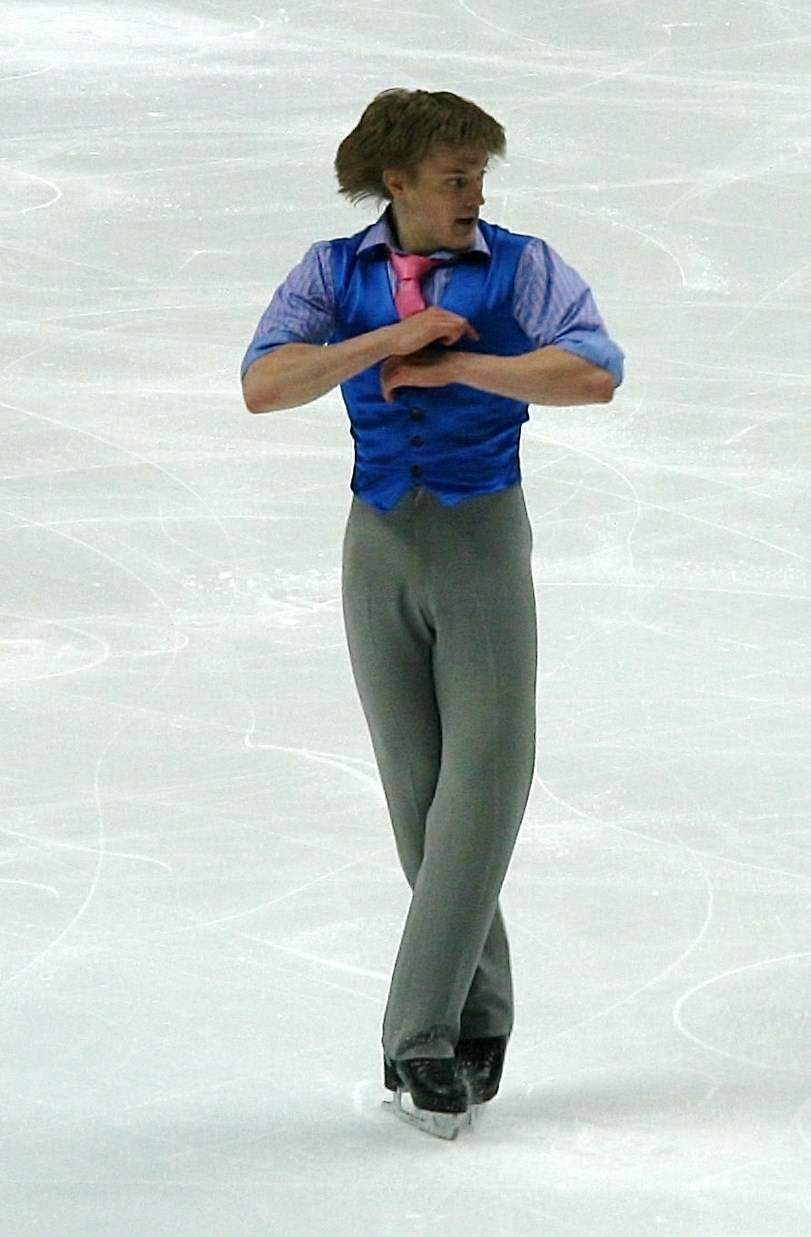
\includegraphics[width=0.3\textwidth]{chapters/chp4_pics/skater.jpg}
\caption{\textit{A skater performs a spin and holds his arms in to increase rotational motion by reducing moment of inertia.}}
\label{fig:skater}
\end{figure}

\noindent Consider a flywheel in an engine. When designed with a larger moment of inertia, it more effectively smooths out the engine's power delivery by storing and releasing rotational energy. This application shows why the $r^2$ term appears in polar form: mass at twice the radius contributes four times as much to the moment of inertia. Engineers use these calculations to design flywheels that achieve the desired balance between energy storage capacity and overall weight. \\

\noindent Moments of inertia appear in several key equations in physics:
\begin{itemize}
   \item Rotational Kinetic Energy: $E = \frac{1}{2}I\omega^2$, where $\omega$ is angular velocity
   \item Torque: $\tau = I\alpha$, where $\alpha$ is angular acceleration \index{Torque}
   \item Angular Momentum: $L = I\omega$ \index{Angular Momentum}
   \item Period of Rotation: $T = 2\pi\sqrt{\frac{I}{k}}$ for a torsional oscillator with spring constant $k$
\end{itemize}

\exampleline
\begin{example}
Elijah the Prophet, a legendary DJ, is designing a custom turntable platter—the rotating disc that holds vinyl records. The platter is shaped like an annular region (a washer shape) with inner radius $r = 1$ inch and outer radius $r = 6$ inches. To ensure smooth playback, the platter's density increases quadratically with radius according to $\rho(r) = kr^2$ ounces/inch$^2$, where $k$ is a constant. If the total mass of the platter is 20 ounces:

\begin{enumerate}
   \item Find the value of $k$.
   \item Calculate the moment of inertia $I_z$ about the turntable's axis of rotation.
   \item If the turntable spins at $33\frac{1}{3}$ RPM (rotations per minute), find its rotational kinetic energy in inch-ounces.
\end{enumerate}

\begin{solution}
\begin{enumerate}
   \item First, let's find $k$ using the total mass equation in polar coordinates:
   \[
   M = \int_0^{2\pi} \int_1^6 \rho(r)r\,dr\,d\theta = \int_0^{2\pi} \int_1^6 kr^3\,dr\,d\theta = 20
   \]
   
   Evaluating the integrals:
   \[
   2\pi k \left[\frac{r^4}{4}\right]_1^6 = 20
   \]
   \[
   2\pi k \left(\frac{1296}{4} - \frac{1}{4}\right) = 20
   \]
   \[
   2\pi k(324 - \frac{1}{4}) = 20
   \]
   
   Therefore:
   \[
   k = \frac{20}{2\pi(323.75)} \approx 0.0098 \text{ oz/inch}^4
   \]

   \item The moment of inertia about the $z$-axis is:
   \[
   I_z = \int_0^{2\pi} \int_1^6 r^2\rho(r)r\,dr\,d\theta = \int_0^{2\pi} \int_1^6 kr^5\,dr\,d\theta
   \]
   
   Substituting our value of $k$:
   \[
   I_z = 2\pi k \left[\frac{r^6}{6}\right]_1^6 = 2\pi \cdot \frac{20}{2\pi(323.75)} \cdot \left(\frac{46656}{6} - \frac{1}{6}\right)
   \]
   \[
   I_z = \frac{20}{323.75} \cdot 7776 \approx 480 \text{ oz}\cdot\text{inch}^2
   \]

   \item The angular velocity at $33\frac{1}{3}$ RPM is:
   \[
   \omega = \frac{100}{3} \cdot \frac{2\pi}{60} = \frac{10\pi}{9} \text{ rad/s}
   \]
   
   The rotational kinetic energy is:
   \[
   E = \frac{1}{2}I_z\omega^2 = \frac{1}{2}(480)\left(\frac{10\pi}{9}\right)^2 \approx 2926 \text{ oz}\cdot\text{inch}^2/\text{s}^2
   \]
\end{enumerate}

\noindent This high moment of inertia helps maintain consistent playback speed, as the platter's substantial rotational inertia resists changes in angular velocity. The quadratic density increase toward the outer edge—similar to putting weights around a turntable's perimeter—maximizes this stabilizing effect.
\end{solution}
\end{example}
\exampleline
\begin{example}
A robotic arm at a manufacturing plant rotates components on a flat mounting plate. The rectangular plate measures 40 cm × 30 cm and has a base density of $\rho_0 = 2$ g/cm$^2$. To optimize the rotation dynamics, the plate's density varies according to $\rho(x,y) = \rho_0(1 + \frac{x^2}{100})$ g/cm$^2$, where $x$ is measured in centimeters from the plate's vertical centerline. The system rotates with an initial angular velocity of $\omega_0 = 2\pi$ rad/s but must decelerate to a stop within time $t$ using a constant torque $\tau$.

\begin{enumerate}
   \item Calculate the moment of inertia $I_z$ about the central vertical axis.
   \item Using the rotational form of Newton's Second Law, $\tau = I\alpha$, find the required torque to bring the plate to rest in 3 seconds.
   \item What is the total angular displacement during this deceleration? Use the equation $\theta = \omega_0t + \frac{1}{2}\alpha t^2$.
\end{enumerate}

\begin{solution}
\begin{enumerate}
   \item Setting up coordinates with the origin at the center of the plate, our region is $R = [-20,20] \times [-15,15]$ in centimeters. For $I_z$:
   \[
   I_z = \iint_R (x^2 + y^2)\rho_0\left(1 + \frac{x^2}{100}\right)\,dA
   \]
   \[
   = \rho_0\int_{-20}^{20}\int_{-15}^{15}(x^2 + y^2)\left(1 + \frac{x^2}{100}\right)\,dy\,dx
   \]
   
   Breaking this into parts and evaluating:
   \[
   I_z = 2(754,000) = 1,508,000 \text{ g}\cdot\text{cm}^2
   \]
   
   Converting to SI units:
   \[
   I_z = 1,508,000 \times 10^{-7} = 0.1508 \text{ kg}\cdot\text{m}^2
   \]

   \item For constant deceleration from $\omega_0$ to 0 in time $t$:
   \[
   \alpha = \frac{\omega_\text{final} - \omega_0}{t} = \frac{0 - 2\pi}{3} = -\frac{2\pi}{3} \text{ rad/s}^2
   \]
   
   Using $\tau = I\alpha$:
   \[
   \tau = 0.1508 \cdot \left(-\frac{2\pi}{3}\right) = -0.316 \text{ N}\cdot\text{m}
   \]

   \item For the total angular displacement:
   \[
   \theta = \omega_0t + \frac{1}{2}\alpha t^2 = 2\pi(3) + \frac{1}{2}\left(-\frac{2\pi}{3}\right)(3)^2
   \]
   \[
   = 6\pi - 3\pi = 3\pi \text{ rad} = 540^\circ
   \]
\end{enumerate}
\end{solution}
\end{example}
\exampleline


\subsection*{Average Values over Two-Dimensional Regions} \index{Average Value} \index{Average Distribution}

\noindent We took a sneak peek of this concept when we looked at average efficiency in the previous lecture -- When analyzing quantities that vary over a region, we often need to find their average values. Just as the average of discrete values is found by summing and dividing by the count, the average value of a continuous function $f(x,y)$ over a region $R$ is found by integrating and dividing by the region's area:
\[
f_{avg} = \frac{\iint_R f(x,y)\,dA}{\iint_R dA}
\]

\noindent This formula has a natural physical interpretation: the denominator $\iint_R dA$ represents the total area of region $R$, while the numerator accumulates the value of $f$ over that same region. For example, if $f(x,y)$ represents temperature at each point on a metal plate, this formula gives the plate's average temperature. \\

\noindent For non-uniform materials where density varies across the region, we often use a weighted average:
\[
f_{avg} = \frac{\iint_R f(x,y)\rho(x,y)\,dA}{\iint_R \rho(x,y)\,dA}
\]

\noindent Here, $\rho(x,y)$ acts as a weighting function, giving more importance to regions of higher density. This weighted form finds frequent use in engineering applications, from calculating the center of mass of a plate with varying density to determining average stress in composite materials. \\

\noindent Both formulas extend naturally to polar coordinates through the appropriate change of variables, with $dA = r\,dr\,d\theta$. This proves particularly useful when working with circular or radially symmetric regions where the function or density varies with distance from a central point.

\subsection*{Surface Area and Physical Interfaces} \index{Surface Area}

\noindent The motivation for surface area begins with the arc length formula that we learned in Chapter 2. Recall that for a curve $y = f(x)$, we found its arc length by considering how differential changes in $x$ and $y$ contribute to the length of an infinitesimal segment:
\[
ds = \sqrt{dx^2 + dy^2} = \sqrt{1 + \left(\frac{dy}{dx}\right)^2}\,dx
\]
This gave us the arc length formula $L = \int_a^b \sqrt{1 + \left(\frac{dy}{dx}\right)^2}\,dx$. \\

\noindent For a surface $z = f(x,y)$, we follow similar reasoning. Consider a small patch of surface above a region $dA$ in the $xy$-plane. As we move in both $x$ and $y$ directions, the surface rises according to its partial derivatives. The actual area of this patch must account for these slopes in both directions, leading to:
\[
dA_{\text{surface}} = \sqrt{1 + \left(\frac{\partial f}{\partial x}\right)^2 + \left(\frac{\partial f}{\partial y}\right)^2}\,dA
\]

\noindent Integrating over the region $R$ gives us the total surface area:
\[
A = \iint_R \sqrt{1 + \left(\frac{\partial f}{\partial x}\right)^2 + \left(\frac{\partial f}{\partial y}\right)^2}\,dA
\]


\begin{figure}[H]
\centering
\tdplotsetmaincoords{60}{120}

\begin{tikzpicture}[tdplot_main_coords, scale=1.7,
declare function={
    surfacefn(\x,\y)=1+0.2*sin(deg(2*\x))*cos(deg(2*\y));
}]

% Axes
\draw[->] (0,0,0) -- (3,0,0) node[right] {$x$};
\draw[->] (0,0,0) -- (0,3,0) node[right] {$y$};
\draw[->] (0,0,0) -- (0,0,2) node[above] {$z$};

% Surface grid
\foreach \x in {0,0.5,...,3} {
    \draw[blue!20] plot[variable=\y,domain=0:3,samples=30] 
    (\x,\y,{surfacefn(\x,\y)});
}
\foreach \y in {0,0.5,...,3} {
    \draw[blue!20] plot[variable=\x,domain=0:3,samples=30] 
    (\x,\y,{surfacefn(\x,\y)});
}

% Surface element parameters
\def\px{1.0}
\def\py{1.0}
\def\dxsize{0.4}
\def\dysize{0.4}

% Surface element corners
\coordinate (P1) at (\px,\py,{surfacefn(\px,\py)});
\coordinate (P2) at ({\px+\dxsize},\py,{surfacefn(\px+\dxsize,\py)});
\coordinate (P3) at ({\px+\dxsize},{\py+\dysize},{surfacefn(\px+\dxsize,\py+\dysize)});
\coordinate (P4) at (\px,{\py+\dysize},{surfacefn(\px,\py+\dysize)});

% Fill surface element
\fill[blue!40,opacity=0.6] (P1) -- (P2) -- (P3) -- (P4) -- cycle;

% Draw element edges
\draw[blue,thick] (P1) -- (P2) -- (P3) -- (P4) -- cycle;

% Tangent vectors u and v
\draw[->,ultra thick,orange] (P1) -- (P2) node[midway, above, sloped] {};
\draw[->,ultra thick,green] (P1) -- (P4) node[midway, left] {};

% Normal vector (cross product)
\draw[->,ultra thick,red] ($(P1)!0.5!(P3)$) --
    ($(P1)!0.5!(P3) + (0,0,0.5)$) node[midway, right] {};

\node at (0,2,2) {$z=f(x,y)$};

% Legend outside the plot area to the right
\node[draw, anchor=west, fill=white, opacity=0.9, right=of current bounding box.east, xshift=0.5cm] {
    \begin{tabular}{ll}
        \textcolor{orange}{$\longrightarrow$} & $\vec{u}$ \\
        \textcolor{green}{$\longrightarrow$} & $\vec{v}$ \\
        \textcolor{red}{$\longrightarrow$} & $\vec{u} \times \vec{v}$ \\
        \textcolor{blue}{\rule{1cm}{2pt}} & $dS$ \\
    \end{tabular}
};

\end{tikzpicture}
\caption{\textit{The surface area element $dS$ arises from the cross product of tangent vectors 
$\vec{u} = (dx, 0, \frac{\partial f}{\partial x}dx)$ and $\vec{v} = (0, dy, \frac{\partial f}{\partial y}dy)$. 
Their cross product gives $dS = \|\vec{u} \times \vec{v}\| = \sqrt{1 + \left(\frac{\partial f}{\partial x}\right)^2 + \left(\frac{\partial f}{\partial y}\right)^2}\,dx\,dy$.}}
\end{figure}


\noindent If our surface is better described using polar coordinates, we can transform this formula. For $z = f(r,\theta)$, the surface area becomes:
\[
A = \iint_R \sqrt{1 + \left(\frac{\partial f}{\partial r}\right)^2 + \frac{1}{r^2}\left(\frac{\partial f}{\partial \theta}\right)^2}\,r\,dr\,d\theta
\]

\noindent Thus, this shows us that surface area is just arc-length in three dimensions. This pattern also generalizes. For a \textit{hypersurface} in $n$ dimensions given by a function of $n-1$ variables, the hypersurface area becomes:
\[
A = \int_R \sqrt{1 + \sum_{i=1}^{n-1} \left(\frac{\partial f}{\partial x_i}\right)^2}\,dA
\]

\noindent This generalization finds applications in physics and engineering. The bad thing about these formulae is that the integral is usually too hard to solve, so we will frequently have to rely on numerical methods and/or the all seeing eye: Wolfram Alpha. \\

\noindent Let us now explore these formulae with a concrete example:

\exampleline
\begin{example}
In architecture, hyperbolic paraboloids (saddle surfaces) are used to create striking modern designs that combine aesthetics with structural efficiency. Consider a surface given by $z = \frac{x^2}{4} - \frac{y^2}{9}$ over the region $R = [-1,1] \times [-2,2]$.

\begin{enumerate}
   \item Set up (but do not evaluate) the surface area integral.
   \item Use the fact that this integral evaluates to approximately 8.56 square units to discuss the efficiency of this architectural form.
\end{enumerate}

\begin{solution}
Let's solve this step by step:

\begin{enumerate}
   \item First, we compute the partial derivatives:
   \[
   \frac{\partial z}{\partial x} = \frac{x}{2}, \quad \frac{\partial z}{\partial y} = -\frac{2y}{9}
   \]

   The surface area is given by:
   \[
   A = \iint_R \sqrt{1 + \left(\frac{\partial z}{\partial x}\right)^2 + \left(\frac{\partial z}{\partial y}\right)^2}\,dA
   \]

   Substituting the partial derivatives:
   \[
   A = \iint_R \sqrt{1 + \frac{x^2}{4} + \frac{4y^2}{81}}\,dA
   \]

   Since the integrand $\sqrt{1 + \frac{x^2}{4} + \frac{4y^2}{81}}$ is even in both $x$ and $y$, we can integrate over the first quadrant and multiply by 4:
   \[
   A = 4\int_0^1\int_0^2 \sqrt{1 + \frac{x^2}{4} + \frac{4y^2}{81}}\,dy\,dx
   \]

   \item The numerical evaluation of this integral yields $A \approx 8.56$ square units. This relatively small surface area compared to the region covered ($8$ square units in the $xy$-plane) demonstrates why hyperbolic paraboloids are efficient architectural forms. The surface area is only about 7\% more than the flat projection, making them materially economical while their curvature provides structural advantages through geometric stiffness.
\end{enumerate}
\end{solution}
\end{example}
\exampleline


\newpage


\lecture{Triple Integrals}

\noindent Imagine you need to find the total mass of an irregularly shaped rock whose density varies throughout, or the total charge inside a thundercloud. These are naturally three-dimensional problems that require integrating a function over a solid region -- and that is exactly what triple integrals do.\\ \\

\noindent Having explored integration over regions in the plane, we now extend our understanding to higher dimensions. Recall that double integrals allowed us to find areas under surfaces by integrating a function $f(x,y)$ over a region $R$, producing outputs in units of ``function $\times$ area''. For instance, when integrating a constant height function $f(x,y) = h$ over a region $R$, we obtained volume: $V = h\iint_R dA$. \\

\noindent Triple integrals follow this pattern but work in three dimensions. When we integrate a function $f(x,y,z)$ over a solid region $E$ in space, our output will have units of ``function $\times$ volume''. At first glance, this might suggest we are limited to producing quantities measured in spatial units to the fourth power—a type of hypervolume. However, just as we saw with density functions producing mass ($\text{g/cm}^3 \times \text{cm}^3 = \text{g}$), the integrand can carry rates that combine with volume in various ways. \\

\noindent Consider, for example, the second moment of inertia tensor in engineering, which has units of $\text{kg}\cdot\text{m}^2$. When analyzing rotating bodies, we might integrate $\rho(x,y,z)(y^2 + z^2)$ to find the moment of inertia about the $x$-axis. Here, the density ($\text{kg}/\text{m}^3$) combines with squared distance terms ($\text{m}^2$) and volume ($\text{m}^3$) to produce the correct units. Or in dynamics, when studying jerk (the rate of change of acceleration), we might integrate a function with units $\text{m}/\text{s}^3$ over a volume to find total change in momentum rate. The power of triple integrals lies in this flexibility to handle various physical quantities through appropriate choice of integrand, practical implications of which will be explored in more detail in the coming lectures in this chapter. The good news for us in this introduction is that we will use almost identical machinery to what we used with double integrals -- there are not many more layers of complexity to add when generalizing double integrals to triple and beyond.


\subsection*{Definition and Computation}

\noindent Consider a solid region $E$ in three-dimensional space and a function $f(x,y,z)$ defined over this region. Just as we built double integrals from the concept of summing over rectangles, we construct triple integrals by summing over small rectangular boxes called volume elements. Each volume element has dimensions $\Delta x$, $\Delta y$, and $\Delta z$, giving it a volume of $\Delta V = \Delta x\Delta y\Delta z$. \\

\noindent When constructing our Riemann sum, we must choose a sample point $(x_i^*, y_i^*, z_i^*)$ within each box. Where single integrals required choosing a point on a line segment and double integrals required choosing a point in a rectangle, triple integrals require selecting a point within a rectangular box. This point could be at any corner of the box (there are eight corners), at the center of the box, or at any other location within the box. For each such box with its chosen sample point, we compute $f(x_i^*, y_i^*, z_i^*)\Delta V_i$. \\

\noindent As all dimensions of these boxes approach zero (that is, as $\Delta x$, $\Delta y$, and $\Delta z$ all approach zero), their sum approaches the triple integral:
\[
\iiint_E f(x,y,z)\,dV = \lim_{n \to \infty} \sum_{i=1}^n f(x_i^*, y_i^*, z_i^*)\Delta V_i
\]

\noindent Just as with double integrals, different choices of sample points might give different approximations, but all reasonable choices converge to the same limit as the box dimensions approach zero. The differential volume element $dV = dx\,dy\,dz$ represents the limiting case of $\Delta V$ as all dimensions approach zero. The units of $dV$ will always be cubic units (cubic meters, cubic centimeters, etc.), while the units of $f(x,y,z)$ could vary depending on the application. \\

\noindent For a rectangular box $E = [a,b] \times [c,d] \times [p,q]$, we can write an iterated integral:
\[
\iiint_E f(x,y,z)\,dV = \int_a^b\int_c^d\int_p^q f(x,y,z)\,dz\,dy\,dx
\]

\noindent This can be evaluated in any order—Fubini's Theorem extends naturally to three dimensions:
\[
\int_a^b\int_c^d\int_p^q f(x,y,z)\,dz\,dy\,dx = \int_p^q\int_c^d\int_a^b f(x,y,z)\,dx\,dy\,dz
\]
and similarly for any other permutation of the variables. The choice of order, while not affecting the result, often significantly impacts the complexity of computation. \\

\noindent For example, if we're computing the mass of a solid where density varies with height, integrating with respect to $z$ first might simplify our work. If instead the density varies with distance from an axis, we might prefer cylindrical coordinates—a system we'll explore shortly.


\subsection*{Types of Integration Regions} \index{Triple Integral Regions}   

\noindent When integrating over general three-dimensional regions, we must carefully analyze the geometry to determine appropriate bounds of integration. Just as with double integrals, we can often view a region from different perspectives, leading to distinct but equivalent ways to set up our integral. Let's examine the three fundamental types of regions we encounter. \\

\noindent \textbf{Type I Regions:} \index{Triple Integral Regions!Type I Regions} These regions are defined by viewing the solid from the side, looking perpendicular to the $xy$-plane. The region is bounded above and below by surfaces $z = g_2(x,y)$ and $z = g_1(x,y)$ respectively, where these surfaces sit above a region $R$ in the $xy$-plane. For such regions:
\[
\iiint_E f(x,y,z)\,dV = \iint_R\int_{g_1(x,y)}^{g_2(x,y)} f(x,y,z)\,dz\,dA
\]

\begin{figure}[H]
\centering
\tdplotsetmaincoords{60}{120} % Adjust viewing angle for Type I
\begin{tikzpicture}[tdplot_main_coords, scale=3]
    % Define coordinates
    \coordinate (O) at (0,0,0);
    \coordinate (A) at (1,0,0);
    \coordinate (B) at (1,1,0);
    \coordinate (C) at (0,1,0);
    
    % Base rectangle R in xy-plane
    \draw[thick, fill=gray!20, opacity=0.5] (0,0,0) -- (1,0,0) -- (1,1,0) -- (0,1,0) -- cycle;
    
    % Bottom surface z = g1(x,y)
    \draw[thick, fill=blue!20, opacity=0.5] (0,0,0) -- (1,0,0) -- (1,1,0) -- (0,1,0) -- cycle;
    
    % Top surface z = g2(x,y)
    \draw[thick, fill=red!20, opacity=0.5] (0,0,1) -- (1,0,1) -- (1,1,1) -- (0,1,1) -- cycle;
    
    % Connect base to top with dashed lines
    \draw[thick, dashed] (0,0,0) -- (0,0,1);
    \draw[thick, dashed] (1,0,0) -- (1,0,1);
    \draw[thick, dashed] (1,1,0) -- (1,1,1);
    \draw[thick, dashed] (0,1,0) -- (0,1,1);
    
    % Axes
    \draw[thick,->] (0,0,0) -- (1.5,0,0) node[anchor=north east]{$x$};
    \draw[thick,->] (0,0,0) -- (0,1.5,0) node[anchor=north west]{$y$};
    \draw[thick,->] (0,0,0) -- (0,0,1.5) node[anchor=south]{$z$};
    
    % Labels
    \node at (0.3,0.3,0) {$R$};
    \node at (0.5,0.5,1.1) {$z = g_2(x,y)$};
    \node at (0.5,0.5,-0.1) {$z = g_1(x,y)$};
\end{tikzpicture}
\caption{\textit{A Type I region bounded by two surfaces above a region $R$ in the $xy$-plane.}}
\end{figure}
 \index{Triple Integral Regions!Type II Regions} 
\noindent \textbf{Type II Regions:} These regions are viewed by looking perpendicular to the $yz$-plane, bounded by surfaces $x = h_1(y,z)$ and $x = h_2(y,z)$ over a region $R$ in the $yz$-plane. Here:
\[
\iiint_E f(x,y,z)\,dV = \iint_R\int_{h_1(y,z)}^{h_2(y,z)} f(x,y,z)\,dx\,dA
\]

\begin{figure}[H]
\centering
\tdplotsetmaincoords{60}{60} % Existing correct view for Type II
\begin{tikzpicture}[tdplot_main_coords, scale=3]

    % Define coordinates
    \coordinate (O) at (0,0,0);
    \coordinate (A) at (1,0,0);
    \coordinate (B) at (1,1,0);
    \coordinate (C) at (0,1,0);
    
    % Base rectangle R in yz-plane
    \draw[thick, fill=gray!20, opacity=0.5] (0,0,0) -- (0,1,0) -- (0,1,1) -- (0,0,1) -- cycle;
    
    % Bottom surface x = h1(y,z) (x = 0)
    \draw[thick, fill=blue!20, opacity=0.5] (0,0,0) -- (0,1,0) -- (0,1,1) -- (0,0,1) -- cycle;
    
    % Top surface x = h2(y,z) (x = 1)
    \draw[thick, fill=red!20, opacity=0.5] (1,0,0) -- (1,1,0) -- (1,1,1) -- (1,0,1) -- cycle;
    
    % Connect base to top with dashed lines
    \draw[thick, dashed] (0,0,0) -- (1,0,0);
    \draw[thick, dashed] (0,1,0) -- (1,1,0);
    \draw[thick, dashed] (0,1,1) -- (1,1,1);
    \draw[thick, dashed] (0,0,1) -- (1,0,1);
    
    % Axes
    \draw[thick,->] (0,0,0) -- (1.5,0,0) node[anchor=north east]{$x$};
    \draw[thick,->] (0,0,0) -- (0,1.5,0) node[anchor=north west]{$y$};
    \draw[thick,->] (0,0,0) -- (0,0,1.5) node[anchor=south]{$z$};
    
    % Labels
    \node at (0,0.3,0.3) {$R$};
    \node at (1.5,0.1,0.5) {$x = h_2(y,z)$};
    \node at (-0.2,0.6,0.5) {$x = h_1(y,z)$};

\end{tikzpicture}
\caption{\textit{A Type II region bounded by surfaces viewed from the $yz$-plane.}}
\end{figure}
 \index{Triple Integral Regions!Type III Regions} 
\noindent \textbf{Type III Regions:} These regions are viewed by looking perpendicular to the $xz$-plane, bounded by surfaces $y = k_1(x,z)$ and $y = k_2(x,z)$ over a region $R$ in the $xz$-plane:
\[
\iiint_E f(x,y,z)\,dV = \iint_R\int_{k_1(x,z)}^{k_2(x,z)} f(x,y,z)\,dy\,dA
\]

\begin{figure}[H]
\centering
\tdplotsetmaincoords{60}{30} % Adjust viewing angle for Type III
\begin{tikzpicture}[tdplot_main_coords, scale=3]
    % Define coordinates
    \coordinate (O) at (0,0,0);
    \coordinate (A) at (1,0,0);
    \coordinate (B) at (1,0,1);
    \coordinate (C) at (0,0,1);
    
    % Base rectangle R in xz-plane
    \draw[thick, fill=gray!20, opacity=0.5] (0,0,0) -- (1,0,0) -- (1,0,1) -- (0,0,1) -- cycle;
    
    % Bottom surface y = k1(x,z)
    \draw[thick, fill=blue!20, opacity=0.5] (0,0,0) -- (1,0,0) -- (1,0,1) -- (0,0,1) -- cycle;
    
    % Top surface y = k2(x,z)
    \draw[thick, fill=red!20, opacity=0.5] (0,1,0) -- (1,1,0) -- (1,1,1) -- (0,1,1) -- cycle;
    
    % Connect base to top with dashed lines
    \draw[thick, dashed] (0,0,0) -- (0,1,0);
    \draw[thick, dashed] (1,0,0) -- (1,1,0);
    \draw[thick, dashed] (1,0,1) -- (1,1,1);
    \draw[thick, dashed] (0,0,1) -- (0,1,1);
    
    % Axes
    \draw[thick,->] (0,0,0) -- (1.5,0,0) node[anchor=north east]{$x$};
    \draw[thick,->] (0,0,0) -- (0,3,0) node[anchor=north west]{$y$};
    \draw[thick,->] (0,0,0) -- (0,0,1.5) node[anchor=south]{$z$};
    
    % Labels
    \node at (0.5,0,0.45) {$R$};
    \node at (1.5,1.1,0.5) {$y = k_2(x,z)$};
    \node at (0.65,-0.1,0.3) {$y = k_1(x,z)$};
\end{tikzpicture}
\caption{\textit{A Type III region bounded by surfaces viewed from the $xz$-plane.}}
\end{figure}


\exampleline
\begin{example}
\begin{enumerate}
   \item Find $\displaystyle\iiint_E (x^2 + y^2)\,dV$ where $E$ is the rectangular box $[0,1] \times [1,2] \times [-1,3]$.
   \item Find $\displaystyle\iiint_E xyz\,dV$ where $E$ is the region bounded below by the $xy$-plane ($z = 0$) and above by the plane $z = 2 - x - y$ in the first octant.
\end{enumerate}

\begin{solution}
\begin{enumerate}
   \item For the rectangular box:

   \begin{figure}[H]
   \centering
   \tdplotsetmaincoords{60}{110}
   \begin{tikzpicture}[tdplot_main_coords,scale=.9]
       % Axes for rectangular box
       \draw[->] (0,0,0) -- (2,0,0) node[right] {$x$};
       \draw[->] (0,0,0) -- (0,3,0) node[right] {$y$};
       \draw[->] (0,0,0) -- (0,0,4) node[left] {$z$};
       
       % Draw back faces (drawn first)
       \fill[blue!20,opacity=0.3] (0,2,-1) -- (0,2,3) -- (1,2,3) -- (1,2,-1) -- cycle;
       \fill[blue!20,opacity=0.3] (1,1,-1) -- (1,2,-1) -- (1,2,3) -- (1,1,3) -- cycle;
       
       % Draw bottom
       \fill[blue!30,opacity=0.3] (0,1,-1) -- (1,1,-1) -- (1,2,-1) -- (0,2,-1) -- cycle;
       
       % Draw front faces
       \fill[blue!40,opacity=0.3] (0,1,-1) -- (0,1,3) -- (0,2,3) -- (0,2,-1) -- cycle;
       \fill[blue!40,opacity=0.3] (0,1,-1) -- (1,1,-1) -- (1,1,3) -- (0,1,3) -- cycle;
       
       % Draw top
       \fill[blue!50,opacity=0.3] (0,1,3) -- (1,1,3) -- (1,2,3) -- (0,2,3) -- cycle;
       
       % Draw edges
       \draw[blue,thick] (0,1,-1) -- (1,1,-1) -- (1,2,-1) -- (0,2,-1) -- cycle;
       \draw[blue,thick] (0,1,3) -- (1,1,3) -- (1,2,3) -- (0,2,3) -- cycle;
       \draw[blue,thick] (0,1,-1) -- (0,1,3);
       \draw[blue,thick] (1,1,-1) -- (1,1,3);
       \draw[blue,thick] (1,2,-1) -- (1,2,3);
       \draw[blue,thick] (0,2,-1) -- (0,2,3);
       
       % Labels for bounds
       \node[below] at (0.5,1.5,-1.4) {$[0,1] \times [1,2] \times [-1,3]$};
   \end{tikzpicture}
   \caption{\textit{Problem 1: Rectangular box region}}
   \end{figure}

   \begin{align*}
   \iiint_E (x^2 + y^2)\,dV &= \int_0^1\int_1^2\int_{-1}^3 (x^2 + y^2)\,dz\,dy\,dx \\[1ex]
   &= \int_0^1\int_1^2 (x^2 + y^2)[z]_{-1}^3\,dy\,dx \\[1ex]
   &= 4\int_0^1\int_1^2 (x^2 + y^2)\,dy\,dx \\[1ex]
   &= 4\int_0^1 \left[x^2y + \frac{y^3}{3}\right]_1^2\,dx \\[1ex]
   &= 4\int_0^1 \left(x^2(2-1) + \frac{8}{3} - \frac{1}{3}\right)\,dx \\[1ex]
   &= 4\left[\frac{x^3}{3} + \frac{7x}{3}\right]_0^1 = \frac{32}{3}
   \end{align*}

   \item For the region in the first octant:

   \begin{figure}[H]
   \centering
   \tdplotsetmaincoords{60}{110}
   \begin{tikzpicture}[tdplot_main_coords,scale=1.2]
       % Axes for slanted plane region
       \draw[->] (0,0,0) -- (3,0,0) node[right] {$x$};
       \draw[->] (0,0,0) -- (0,3,0) node[right] {$y$};
       \draw[->] (0,0,0) -- (0,0,3) node[left] {$z$};
       
       % Fill base triangle
       \fill[blue!20,opacity=0.3] (0,0,0) -- (2,0,0) -- (0,2,0) -- cycle;
       
       % Fill side faces
       \fill[blue!30,opacity=0.3] (0,0,0) -- (2,0,0) -- (2,0,0) -- (0,0,2) -- cycle;
       \fill[blue!30,opacity=0.3] (0,0,0) -- (0,2,0) -- (0,0,2) -- cycle;
       \fill[blue!40,opacity=0.3] (0,0,2) -- (2,0,0) -- (0,2,0) -- cycle;
       
       % Draw edges
       \draw[blue,thick] (0,0,0) -- (2,0,0) -- (0,2,0) -- cycle;
       \draw[blue,thick] (0,0,0) -- (0,0,2);
       \draw[blue,thick,dashed] (0,0,2) -- (2,0,0);
       \draw[blue,thick,dashed] (0,0,2) -- (0,2,0);
       
       % Label the plane
       \node at (1,3,1.5) {$z = 2-x-y$};
       \node at (0.5,0.5,0) {$z = 0$};
   \end{tikzpicture}
   \caption{\textit{Problem 2: Region bounded by plane $z = 2-x-y$ and $xy$-plane}}
   \end{figure}

\noindent The bounds are in the first octant bounded below by the $xy$-plane ($z=0$) and above by the plane $z=2-x-y$. From the $xy$-plane projection, we see $x$ ranges from $0$ to $2$, and for each fixed $x$, $y$ ranges from $0$ to $2-x$. For each fixed $x$ and $y$, $z$ then ranges from $0$ to $2-x-y$, giving the triple integral's bounds.

   \begin{align*}
   \iiint_E xyz\,dV &= \int_0^2\int_0^{2-x}\int_0^{2-x-y} xyz\,dz\,dy\,dx \\[1ex]
   &= \int_0^2\int_0^{2-x} xy\left[\frac{z^2}{2}\right]_0^{2-x-y}\,dy\,dx \\[1ex]
   &= \frac{1}{2}\int_0^2\int_0^{2-x} xy(2-x-y)^2\,dy\,dx
   \end{align*}
   
   Let $u = 2-x-y$, so $y = 2-x-u$ and $dy = -du$. When $y = 0$, $u = 2-x$; when $y = 2-x$, $u = 0$. This gives:
   \begin{align*}
   &= \frac{1}{2}\int_0^2 x\int_{2-x}^0 (2-x-u)u^2(-du)\,dx \\[1ex]
   &= \frac{1}{2}\int_0^2 x\left[(2-x)\frac{u^3}{3} - \frac{u^4}{4}\right]_0^{2-x}\,dx \\[1ex]
   &= \frac{1}{24}\int_0^2 x(2-x)^4\,dx = \frac{4}{45}
   \end{align*}
\end{enumerate}
\end{solution}
\end{example}
\exampleline

\begin{example}
Find $\displaystyle\iiint_E 1\,dV$ where $E$ is the region bounded by the intersection of two perpendicular unit cylinders $x^2 + y^2 = 1$ and $x^2 + z^2 = 1$.

\begin{solution}

%https://commons.wikimedia.org/wiki/File:Steinmetz-cc.svg
%https://commons.wikimedia.org/wiki/File:Steinmetz-cc2-ag.svg
\begin{figure}[H]
\centering
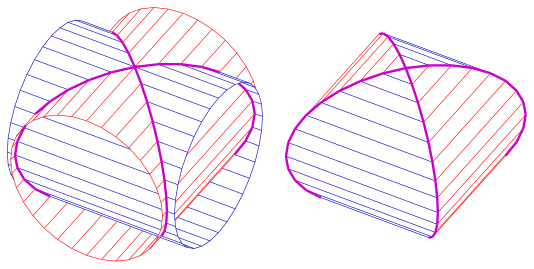
\includegraphics[width=0.6\textwidth]{chapters/chp4_pics/steinmetz.png}
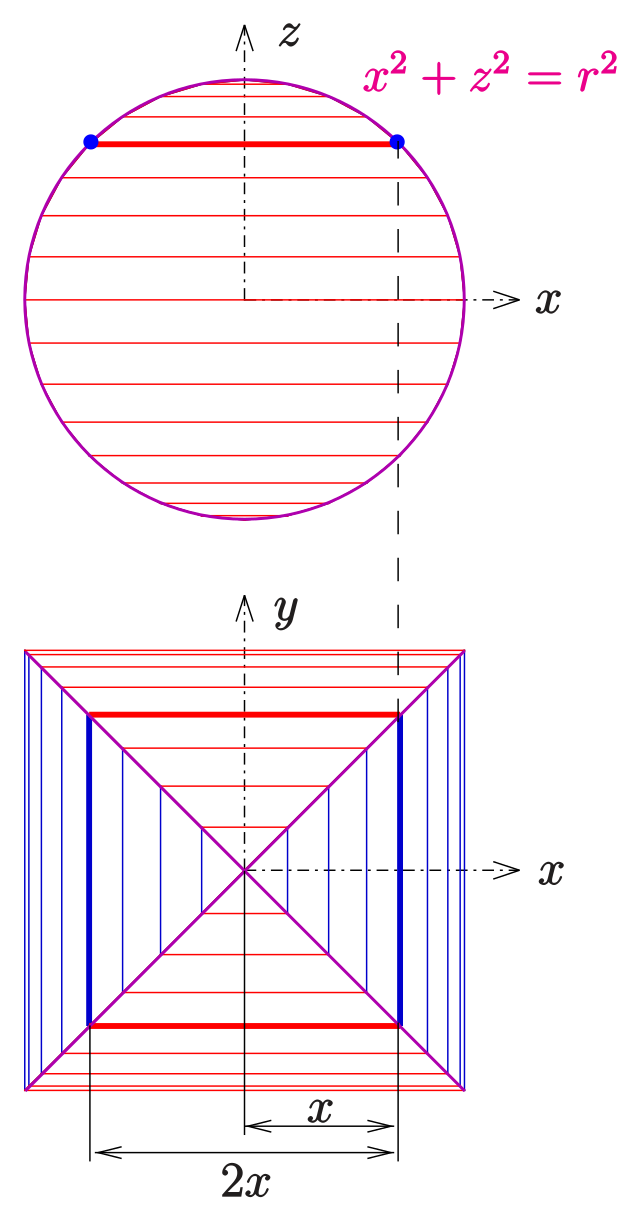
\includegraphics[width=0.25\textwidth]{chapters/chp4_pics/steinmetz-side.png}
\caption{\textit{The Steinmetz solid, formed by the intersection of two perpendicular unit cylinders $x^2 + y^2 = 1$ and $x^2 + z^2 = 1$.}}
\label{fig:steinmetz}
\end{figure}

\noindent Due to the symmetry of the region across all coordinate planes, we can evaluate the integral in the first octant and multiply by 8. In the first octant, $x$ ranges from $0$ to $1$, and for each fixed $x$, both $y$ and $z$ range from $0$ to $\sqrt{1-x^2}$ due to the circular cross-sections of the cylinders (found by solving our two equations for $y$ and $z$):
\begin{align*}
\iiint_E 1\,dV &= 8\int_0^1\int_0^{\sqrt{1-x^2}}\int_0^{\sqrt{1-x^2}} 1\,dz\,dy\,dx \\[1ex]
&= 8\int_0^1\int_0^{\sqrt{1-x^2}} \sqrt{1-x^2}\,dy\,dx \\[1ex]
&= 8\int_0^1 (1-x^2)\,dx \\[1ex]
&= 8\left[x - \frac{x^3}{3}\right]_0^1 = 8\left(1 - \frac{1}{3}\right) = \frac{16}{3}
\end{align*}
\end{solution}
\end{example}
\exampleline

\noindent The choice of which type to use for a given region often depends on the geometry of the bounding surfaces and the nature of the integrand. Many complex regions might require breaking the integral into parts and using different types for each part. Just as with double integrals, the goal is to choose the type that leads to the most straightforward computation. \\

\noindent However, for certain geometries—particularly those with circular or spherical symmetry—we'll find that alternative coordinate systems provide more natural representations. These systems, cylindrical and spherical coordinates, will be our next topic of study.

\subsection*{Coordinate Systems for Triple Integration}

\noindent The choice of coordinate system can dramatically simplify a triple integral computation. Just as we found polar coordinates useful for double integrals over circular regions, cylindrical and spherical coordinates provide natural frameworks for three-dimensional regions with certain types of symmetry. Let's examine these alternative coordinate systems and understand how they transform our integration process.

\subsubsection*{Cylindrical Coordinates}

\noindent As we learned in Chapter 1, cylindrical coordinates extend polar coordinates into three dimensions by adding a height coordinate. A point $(x,y,z)$ in rectangular coordinates is represented by coordinates $(r,\theta,z)$ in the cylindrical system:
\begin{align*}
x &= r\cos\theta \\
y &= r\sin\theta \\
z &= z
\end{align*}

\noindent The coordinate $r$ represents the distance from the point to the $z$-axis, $\theta$ measures the angle from the positive $x$-axis in the $xy$-plane, and $z$ gives the height above the $xy$-plane. This system naturally describes surfaces like cylinders, where $r$ is constant, and cones, where $z$ is proportional to $r$. \\

\noindent When converting a triple integral to cylindrical coordinates, we must account for how volume elements transform. A small rectangular box $dx\,dy\,dz$ becomes a curved wedge $r\,dr\,d\theta\,dz$. The factor of $r$ appears for the same reason it did in double integrals—as we move farther from the $z$-axis, the same angular increment $d\theta$ sweeps out a larger arc. Thus:
\[
\iiint_E f(x,y,z)\,dV = \iiint_E f(r\cos\theta, r\sin\theta, z)r\,dr\,d\theta\,dz
\]

\begin{figure}[H]
\centering
%Axis Angles
\tdplotsetmaincoords{70}{110}

%Macros
\pgfmathsetmacro{\rvec}{5}
\pgfmathsetmacro{\phivec}{45}
\pgfmathsetmacro{\zvec}{4}

\pgfmathsetmacro{\drvec}{1.5}
\pgfmathsetmacro{\dphivec}{20}
\pgfmathsetmacro{\dzvec}{1}

%Layers
\pgfdeclarelayer{background}
\pgfdeclarelayer{foreground}

\pgfsetlayers{background, main, foreground}

\begin{tikzpicture}[tdplot_main_coords]

%Coordinates
\coordinate (O) at (0,0,0);
%%
\cylindricalcoordinate{\rvec}{\phivec}{\zvec}{A}
\cylindricalcoordinate{\rvec}{\phivec}{(\zvec+\dzvec)}{B}
\cylindricalcoordinate{\rvec}{(\phivec+\dphivec)}{\zvec}{C}
\cylindricalcoordinate{\rvec}{(\phivec+\dphivec)}{(\zvec+\dzvec)}{D}
%%
\cylindricalcoordinate{(\rvec+\drvec)}{\phivec}{\zvec}{A'}
\cylindricalcoordinate{(\rvec+\drvec)}{\phivec}{(\zvec+\dzvec)}{B'}
\cylindricalcoordinate{(\rvec+\drvec)}{(\phivec+\dphivec)}{\zvec}{C'}
\cylindricalcoordinate{(\rvec+\drvec)}{(\phivec+\dphivec)}{(\zvec+\dzvec)}{D'}
%%%Nodes
%\node at (A) {A};
%\node at (B) {B};
%\node at (C) {C};
%\node at (D) {D};
%\node at (A') {A'};
%\node at (B') {B'};
%\node at (C') {C'};
%\node at (D') {D'};

%Axis
\begin{pgfonlayer}{background}
	\draw[thick,-latex] (0,0,0) -- (6,0,0) node[pos=1.1]{$x$};
	\draw[thick,-latex] (0,0,0) -- (0,6,0) node[pos=1.05]{$y$};
	\draw[thick,-latex] (0,0,0) -- (0,0,6) node[pos=1.05]{$z$};
\end{pgfonlayer}

%Vectors
\begin{pgfonlayer}{main}
	\draw[blue, thick] (O) -- (A);
	\draw[thick] (O) -- (Axy) node [pos=0.6, below left] {$r$};
	\draw (A) -- ($(A)-(Axy)$) node [left] {$z$};
	\draw (B) -- ($(A)-(Axy)+(0,0,\dzvec)$) node [left] {$z+dz$};
	\draw (D) -- ($(A)-(Axy)+(0,0,\dzvec)$);
\end{pgfonlayer}
\begin{pgfonlayer}{background}
	\draw[dashed] (C) -- ($(A)-(Axy)$) node [left] {$z$};
\end{pgfonlayer}

%Help Lines
\begin{pgfonlayer}{background}
	\draw (A) -- (Axy);
	\draw (A') -- (A'xy);
	\draw[thick] (Axy) -- (A'xy) node [pos=0.6, below left] {$dr$};
	%
	\draw (O) -- (D'xy);
	\draw[dashed] (C) -- (Dxy);	
	\draw (C') -- (C'xy);
	%%Arcs
	\tdplotdrawarc{(0,0,0)}{\rvec}{\phivec}{\phivec+\dphivec}{}{}
	\tdplotdrawarc{(0,0,0)}{\rvec+\drvec}{\phivec}{\phivec+\dphivec}{}{}
\end{pgfonlayer}

%Angles
\begin{pgfonlayer}{foreground}
	%Phi, dPhi
	\tdplotdrawarc[-stealth]{(O)}{0.9}{0}{\phivec}{anchor=north}{$\theta$}
	\tdplotdrawarc[-stealth]{(O)}{1.5}{\phivec}{\phivec + \dphivec}{}{}
	\node at (1.4,1.9,0) {$d \theta$};	
\end{pgfonlayer}

%Differential Volume

%%Lines
\begin{pgfonlayer}{foreground}
	\draw[thick] (A) -- (B) -- (B') -- (A') -- cycle node [midway, below] {$dr$};
	\draw[thick] (D) -- (D') -- (C') node [midway, right] {$dz$};
\end{pgfonlayer}
\begin{pgfonlayer}{background}
	\draw[thick, dashed] (C') -- (C) -- (D);
\end{pgfonlayer}

%%Curved
\begin{pgfonlayer}{background}
	\tdplotdrawarc[thick, dashed]{(0,0,\zvec)}{\rvec} {\phivec}{\phivec+\dphivec}{}{}
\end{pgfonlayer}
\begin{pgfonlayer}{foreground}
	\tdplotdrawarc[thick]{(0,0,\zvec+\dzvec)}{\rvec} {\phivec}{\phivec+\dphivec}{}{}
	\node at (2.4,3.4,\zvec+\dzvec) {$r d\theta$};
	\tdplotdrawarc[thick]{(0,0,\zvec+\dzvec)}{\rvec+\drvec} {\phivec}{\phivec+\dphivec}{}{}
	\tdplotdrawarc[thick]{(0,0,\zvec)}{\rvec+\drvec} {\phivec}{\phivec+\dphivec}{}{}
\end{pgfonlayer}

%%Fill Color
\begin{pgfonlayer}{main}
	%Front
	\fill[black, opacity=0.15] (B) to (B') to[bend right=4] (D') to (D) to[bend left=4] cycle;
	\fill[black, opacity=0.6] (B') to[bend right=4] (D') to (C') to[bend left=4] (A') to cycle;
	\fill[black, opacity=0.4] (B) to (B')  to (A') to (A) to cycle;
\end{pgfonlayer}
\begin{pgfonlayer}{background}
	%Back
	\fill[black!50, opacity=0.5] (D) to (D') to (C') to (C) to cycle;
	\fill[black!50, opacity=0.5] (B) to[bend right=4] (D) to (C) to[bend left=4] (A) to cycle;
	\fill[black!50, opacity=0.5] (A) to (A') to[bend right=4] (C') to (C) to[bend left=4] cycle;
\end{pgfonlayer}


\end{tikzpicture}
\caption{\textit{Representation of a volume element in cylindrical coordinates \((r, \theta, z)\), where \(r\) is the radial distance from the \(z\)-axis, \(\theta\) is the azimuthal angle in the \(xy\)-plane, and \(z\) is the height along the \(z\)-axis.}}
\end{figure}

\noindent The bounds of integration depend on the region $E$. Common patterns include:
\begin{align*}
0 &\leq r \leq R & \text{(solid cylinder)} \\
0 &\leq \theta \leq 2\pi & \text{(full revolution)} \\
a &\leq z \leq b & \text{(fixed height)}
\end{align*}

\subsubsection*{Spherical Coordinates}

\noindent Spherical coordinates offer an even more radical departure from rectangular coordinates, particularly useful for regions with spherical symmetry. A point $(x,y,z)$ is represented by coordinates $(\rho,\theta,\phi)$, where:
\begin{align*}
x &= \rho\sin\phi\cos\theta \\
y &= \rho\sin\phi\sin\theta \\
z &= \rho\cos\phi
\end{align*}

\noindent Here, $\rho$ represents the distance from the origin to the point, $\theta$ measures the angle from the positive $x$-axis in the $xy$-plane (as in cylindrical coordinates), and $\phi$ measures the angle from the positive $z$-axis. Note that $\phi$ is often called the polar angle, while $\theta$ is the azimuthal angle. \\

\noindent The volume element transformation in spherical coordinates is more complex than in cylindrical coordinates. A small volume element becomes $\rho^2\sin\phi\,d\rho\,d\theta\,d\phi$. The factor $\rho^2\sin\phi$ can be understood geometrically:
\begin{itemize}
   \item The $\rho^2$ term accounts for the radial growth in three dimensions
   \item The $\sin\phi$ term accounts for the ``thinning" of the volume element near the poles
\end{itemize}

\noindent Therefore, our triple integral becomes:
\[
\iiint_E f(x,y,z)\,dV = \iiint_E f(\rho\sin\phi\cos\theta, \rho\sin\phi\sin\theta, \rho\cos\phi)\rho^2\sin\phi\,d\rho\,d\theta\,d\phi
\]

%https://tikz.net/spherical_volume/     Alexandros Tsagkaropoulos
\begin{figure}[H]
\centering
%Axis Angles
\tdplotsetmaincoords{70}{110}

%Macros
\pgfmathsetmacro{\rvec}{6}
\pgfmathsetmacro{\thetavec}{40}
\pgfmathsetmacro{\phivec}{45}

\pgfmathsetmacro{\dphivec}{20}
\pgfmathsetmacro{\dthetavec}{20}
\pgfmathsetmacro{\drvec}{1.5}

%Layers
\pgfdeclarelayer{background}
\pgfdeclarelayer{foreground}

\pgfsetlayers{background, main, foreground}

\begin{tikzpicture}[tdplot_main_coords]

%Coordinates
\coordinate (O) at (0,0,0);
%
\tdplotsetcoord{A}{\rvec}{\thetavec}{\phivec}
\tdplotsetcoord{B}{\rvec}{\thetavec + \dthetavec}{\phivec}
\tdplotsetcoord{C}{\rvec}{\thetavec + \dthetavec}{\phivec + \dphivec}
\tdplotsetcoord{D}{\rvec}{\thetavec}{\phivec + \dphivec}
%
\tdplotsetcoord{E}{\rvec + \drvec}{\thetavec}{\phivec}
\tdplotsetcoord{F}{\rvec + \drvec}{\thetavec + \dthetavec}{\phivec}
\tdplotsetcoord{F'}{\rvec + \drvec}{90}{\phivec}
\tdplotsetcoord{G}{\rvec + \drvec}{\thetavec + \dthetavec}{\phivec + \dphivec}
\tdplotsetcoord{G'}{\rvec + \drvec}{90}{\phivec + \dphivec}
\tdplotsetcoord{H}{\rvec + \drvec}{\thetavec}{\phivec + \dphivec}
%%%Nodes
%\node at (A) {A};
%\node at (B) {B};
%\node at (C) {C};
%\node at (D) {D};
%\node at (E) {E};
%\node at (F) {F};
%\node at (G) {G};
%\node at (H) {H};

%Axis
\begin{pgfonlayer}{background}
	\draw[thick,-latex] (0,0,0) -- (7,0,0) node[pos=1.1]{$x$};
	\draw[thick,-latex] (0,0,0) -- (0,7,0) node[pos=1.05]{$y$};
	\draw[thick,-latex] (0,0,0) -- (0,0,5.5) node[pos=1.05]{$z$};
\end{pgfonlayer}

%Help Lines
\begin{pgfonlayer}{background}
	%Up
	\draw[thick, blue] (O) -- (A) node[pos=0.6, above left, blue] {$\rho$};
	\draw (O) -- (B);
	\draw (O) -- (C);
	\draw[dashed] (O) -- (D);
	%Down
	\draw (O) -- (F');
	\draw (O) -- (G');
\end{pgfonlayer}
\begin{pgfonlayer}{foreground}
	%%Help Curves
	\tdplotsetthetaplanecoords{\phivec}
	\tdplotdrawarc[tdplot_rotated_coords]{(O)}{\rvec}{\thetavec+\dthetavec}{90}{}{}
	\tdplotdrawarc[tdplot_rotated_coords]{(O)}{\rvec+\drvec}{\thetavec+\dthetavec}{90}{}{}
	\tdplotsetthetaplanecoords{\phivec+\dphivec}
	\tdplotdrawarc[tdplot_rotated_coords, dashed]{(O)}{\rvec}{\thetavec+\dthetavec}{90}{}{}
	\tdplotdrawarc[tdplot_rotated_coords]{(O)}{\rvec+\drvec}{\thetavec+\dthetavec}{90}{}{}
	%
	\tdplotdrawarc[tdplot_main_coords]{(O)}{\rvec}{\phivec}{\phivec+\dphivec}{}{}
	\node[rotate=13] at (3,4.45,0) {$\rho \sin(\phi) \, d\theta$};
	\tdplotdrawarc[tdplot_main_coords]{(O)}{\rvec+\drvec}{\phivec}{\phivec+\dphivec}{}{}
\end{pgfonlayer}


%Angles
\begin{pgfonlayer}{foreground}
	%Theta, dTheta (azimuthal angle in xy-plane)
	\tdplotdrawarc[-stealth]{(O)}{0.9}{0}{\phivec}{anchor=north}{$\theta$}
	\tdplotdrawarc[-stealth]{(O)}{1.5}{\phivec}{\phivec + \dphivec}{}{}
	\node at (1.4,1.9,0) {$d \theta$};

	\tdplotsetthetaplanecoords{\phivec}

	%Phi, dPhi (polar angle from z-axis)
	\tdplotdrawarc[tdplot_rotated_coords, -stealth]{(0,0,0)}{1.2}{0}{\thetavec}{}{}
	\node at (0,0.3,1.3) {$\phi$};
	\tdplotdrawarc[tdplot_rotated_coords, -stealth]{(0,0,0)}{2.}{\thetavec}{\thetavec + \dthetavec}{anchor=south west}{$d \phi$}
\end{pgfonlayer}

%Differential Volume

%%Lines
\begin{pgfonlayer}{foreground}
	\draw[thick] (A) -- (E) node[midway, above left]{$d \rho$};
	\draw[thick] (B) -- (F);
	\draw[thick] (C) -- (G);
\end{pgfonlayer}
\begin{pgfonlayer}{background}
	\draw[dashed, thick] (D) -- (H);
\end{pgfonlayer}


%%Curved
\begin{pgfonlayer}{background}
	\tdplotsetrotatedcoords{55}{-50.4313}{-6.4086}
	\tdplotdrawarc[dashed, tdplot_rotated_coords, thick]{(O)}{\rvec}{0}{12.8173}{}{}
	%
	\tdplotsetthetaplanecoords{\phivec + \dphivec}
	\tdplotdrawarc[dashed, tdplot_rotated_coords, thick]{(O)}{\rvec}{\thetavec}{\dthetavec + \thetavec}{}{}
\end{pgfonlayer}
\begin{pgfonlayer}{foreground}
	\tdplotsetthetaplanecoords{\phivec}
	\tdplotdrawarc[tdplot_rotated_coords, thick]{(O)}{\rvec}{\thetavec}{\dthetavec + \thetavec}{below left}{$\rho \, d\phi$}
	\tdplotdrawarc[tdplot_rotated_coords, thick]{(O)}{\rvec + \drvec}{\thetavec}{\dthetavec + \thetavec}{}{}
	%
	\tdplotsetthetaplanecoords{\phivec + \dphivec}
	\tdplotdrawarc[tdplot_rotated_coords, thick]{(O)}{\rvec + \drvec}{\thetavec}{\dthetavec + \thetavec}{}{}
	%
	\tdplotsetrotatedcoords{55}{-50.4313}{-6.4086}
	\tdplotdrawarc[tdplot_rotated_coords, thick]{(O)}{\rvec + \drvec}{0}{12.8173}{}{}
	%
	\tdplotsetrotatedcoords{55}{-30.3813}{-8.6492}
	\tdplotdrawarc[tdplot_rotated_coords, thick]{(O)}{\rvec}{0}{17.2983}{}{}
	\tdplotdrawarc[tdplot_rotated_coords, thick]{(O)}{\rvec + \drvec}{0}{17.2983}{}{}
\end{pgfonlayer}

%Fill Color
\begin{pgfonlayer}{main}
	%Front
	\fill[black, opacity=0.15] (E) to (A)  to[bend left=4] (B) to (F) to[bend right=4] cycle;
	\fill[black, opacity=0.6] (E) to[bend left=4] (F)  to[bend left=2] (G) to[bend right=6.5] (H) to[bend right=4] cycle;
	\fill[black, opacity=0.4] (F) to[bend left=2] (G) to[bend left=1.5] (C) to[bend right=2.5] (B) to[bend right=4] cycle;
	\end{pgfonlayer}
\begin{pgfonlayer}{background}
	%Back
	\fill[black!50, opacity=0.5] (A) to[bend left=2] (D) to[bend left=6] (C) to[bend right=2.5] (B) to[bend right=4] cycle;
	\fill[black!50, opacity=0.5] (A) to[bend left=2] (D) to (H) to[bend right=2.5] (E) to[bend right=4] cycle;
	\fill[black!50, opacity=0.5] (D) to (H) to[bend left=6] (G) to[bend right=2] (C) to[bend right=6] cycle;
\end{pgfonlayer}


\end{tikzpicture}
\caption{\textit{Representation of a volume element in spherical coordinates \((\rho, \theta, \phi)\), where \(\rho\) is the radial distance, \(\theta\) is the azimuthal angle in the \(xy\)-plane, and \(\phi\) is the polar angle from the \(z\)-axis. The volume element is defined by \(\rho^2 \sin\phi \, d\rho \, d\theta \, d\phi\), illustrating the differential components \(d\rho\), \(\rho \, d\phi\), and \(\rho \sin\phi \, d\theta\).}}
\end{figure}

\noindent Typical bounds in spherical coordinates follow these patterns:
\begin{align*}
0 &\leq \rho \leq R & \text{(solid sphere)} \\
0 &\leq \theta \leq 2\pi & \text{(full revolution)} \\
0 &\leq \phi \leq \pi & \text{(full sphere)}
\end{align*}

\noindent \textbf{Common Mistakes:} (1) The polar angle \( \phi \) ranges from \( 0 \) to \( \pi \) (not \( 2\pi \)) -- it sweeps from the north pole to the south pole. For a hemisphere with \( z \geq 0 \), use \( 0 \leq \phi \leq \pi/2 \). (2) Always include the full Jacobian factor \( \rho^2 \sin\phi \) in the volume element -- do not forget the \( \sin\phi \).\\ \\

\noindent The choice between cylindrical and spherical coordinates often depends on the region's geometry and the integrand's form. Cylindrical coordinates excel for regions with circular cross-sections parallel to the $xy$-plane, while spherical coordinates are natural for regions bounded by spheres or cones centered at the origin. Both systems can dramatically simplify integrals that would be challenging in rectangular coordinates, particularly when the integrand involves terms like $\sqrt{x^2 + y^2}$ or $\sqrt{x^2 + y^2 + z^2}$.


\exampleline
\begin{example}
\begin{enumerate}
    \item Find the volume of a right circular cone with height $h$ and radius $r$ using cylindrical coordinates.
    \item Evaluate $\displaystyle\iiint_E (x^2 + y^2 + z^2)\,dV$ where $E$ is the solid sphere of radius 2 centered at the origin.
\end{enumerate}

\begin{solution}
\begin{enumerate}
    \item Let's first visualize what's going on:
\begin{figure}[H]
\centering
\tdplotsetmaincoords{70}{110}
\begin{tikzpicture}[tdplot_main_coords, scale=2]
    % Axes
    \draw[->] (0,0,0) -- (2,0,0) node[anchor=north east]{$x$};
    \draw[->] (0,0,0) -- (0,2,0) node[anchor=north west]{$y$};
    \draw[->] (0,0,0) -- (0,0,2.5) node[anchor=south]{$z$};
    
    % Draw base circle
    \draw[thick] (0,0,0) circle (1.5);
    
    % Draw visible cone edges
    \draw[thick] (0,0,2) -- (1.5,0,0);
    \draw[thick] (0,0,2) -- (-1.5,0,0);
    \draw[thick] (0,0,2) -- (0,1.5,0);
    \draw[thick] (0,0,2) -- (0,-1.5,0);
    
    % Draw base circle
    \draw[thick] (0,0,0) circle (1.5);
    
    % Add dashed height line
    \draw[dashed] (0,0,0) -- (0,0,2);
    
    % Add labels with coordinates
    \draw[<->] (1.5,0,0) -- (1.5,0,2);
    \node at (2,0,1) {$h$};  % height label at (1.7,0,1)
    
    \draw[<->] (0,0,0) -- (1.5,0,0);
    \node at (0.5,0.2,0) {$r$};  % radius label at (0.75,-0.2,0)
    
    % Add a sample cross-section at height z
    \draw[dashed, red] (0.9,0,0.8) arc (0:360:0.9);
    \draw[red, <->] (0,0,0.8) -- (0.9,0,0.8);
    \node[red] at (0.2,1.3,1) {$R(z)$};  % R(z) label at (0.5,0.2,0.8)
    
    \draw[dashed, red] (0,0,0.8) -- (0,0,0);
    \node[red] at (0.3,-0.1,0.8) {$z$};  % z label at (0.3,-0.1,0.8)
    
\end{tikzpicture}
\caption{\textit{A right circular cone of height $h$ and radius $r$. The red dashed circle represents a horizontal cross-section at height $z$ with radius $R(z)$, demonstrating how the radius varies linearly with height.}}
\label{fig:right_circular_cone}
\end{figure}
\noindent For a right circular cone, we first need to understand how the radius varies with height. Consider any horizontal cross-section at height $z$ from the base. This creates two similar triangles: the full cone (radius $r$, height $h$), and the smaller cone above our cross-section (radius $R(z)$, height $h-z$). By the properties of similar triangles:
    
    \[
    \frac{R(z)}{r} = \frac{h-z}{h}
    \]
    
\noindent Solving for $R(z)$, we get $R(z) = \frac{r}{h}(h-z)$. This equation shows that the radius decreases linearly as we move up the cone, becoming zero at the top ($z = h$) and equal to $r$ at the base ($z = 0$). In cylindrical coordinates, we integrate over the angle $\theta$ from $0$ to $2\pi$ as it sweeps around the $xy$-plane, the height $z$ from $0$ to $h$, and for each fixed $z$, the radius $\rho$ from $0$ to $R(z) = \frac{r}{h}(h-z)$:
    
    \begin{align*}
    V &= \iiint_E 1\,dV = \int_0^{2\pi}\int_0^h\int_0^{r(h-z)/h} \rho\,d\rho\,dz\,d\theta \\[1ex]
    &= \int_0^{2\pi}\int_0^h \left[\frac{\rho^2}{2}\right]_0^{r(h-z)/h}\,dz\,d\theta \\[1ex]
    &= \int_0^{2\pi}\int_0^h \frac{r^2(h-z)^2}{2h^2}\,dz\,d\theta \\[1ex]
    &= 2\pi\int_0^h \frac{r^2(h-z)^2}{2h^2}\,dz \\[1ex]
    &= \frac{\pi r^2}{h^2}\int_0^h (h-z)^2\,dz \\[1ex]
    &= \frac{\pi r^2}{h^2}\left[-\frac{(h-z)^3}{3}\right]_0^h \\[1ex]
    &= \frac{\pi r^2}{h^2}\left[0 - \left(-\frac{h^3}{3}\right)\right] = \frac{1}{3}\pi r^2h
    \end{align*}
   \item The integrand $x^2 + y^2 + z^2$ suggests the use of spherical coordinates. Recall the transformations:
   \[
   x = \rho\sin\phi\cos\theta, \quad y = \rho\sin\phi\sin\theta, \quad z = \rho\cos\phi
   \]
   
   The volume element in spherical coordinates is:
   \[
   dV = \rho^2\sin\phi\,d\rho\,d\phi\,d\theta
   \]
   
   \noindent For a sphere centered at the origin with radius $2$, we integrate over the angle $\theta$ from $0$ to $2\pi$, the polar angle $\phi$ from $0$ to $\pi$ to cover the full sphere north to south, and the radius $\rho$ from $0$ to $2$. Thus our integral becomes:
   \begin{align*}
   \iiint_E (x^2 + y^2 + z^2)\,dV &= \iiint_E \rho^2\,dV \\[1ex]
   &= \int_0^{2\pi}\int_0^{\pi}\int_0^2 \rho^2 \cdot \rho^2\sin\phi\,d\rho\,d\phi\,d\theta \\[1ex]
   &= \int_0^{2\pi}\int_0^{\pi}\int_0^2 \rho^4\sin\phi\,d\rho\,d\phi\,d\theta \\[1ex]
   &= \int_0^{2\pi}\int_0^{\pi}\left[\frac{\rho^5}{5}\right]_0^2\sin\phi\,d\phi\,d\theta \\[1ex]
   &= \int_0^{2\pi}\int_0^{\pi}\frac{32}{5}\sin\phi\,d\phi\,d\theta \\[1ex]
   &= \frac{32}{5}\int_0^{2\pi}[-\cos\phi]_0^{\pi}\,d\theta \\[1ex]
   &= \frac{32}{5}\int_0^{2\pi}[(-\cos\pi) - (-\cos 0)]\,d\theta = \frac{128\pi}{5}
   \end{align*}
\end{enumerate}
\end{solution}
\end{example}
\exampleline
\begin{example}
An engineer is designing a cylindrical support beam that needs to be contained entirely within a spherical dome. If the dome has radius $R$ and the beam has radius $a$ (where $a < R$), find the volume of the portion of the beam that lies within the dome. \\

\noindent Mathematically, find the volume of the region bounded by:
\begin{itemize}
   \item Sphere: $x^2 + y^2 + z^2 = R^2$
   \item Cylinder: $x^2 + y^2 = a^2$
\end{itemize}

\begin{solution}
The symmetry of this region suggests using cylindrical coordinates. First, let's understand our bounds: \\

\noindent In cylindrical coordinates:
\begin{itemize}
   \item The cylinder equation becomes $r = a$
   \item The sphere equation becomes $r^2 + z^2 = R^2$, which gives us $z = \pm\sqrt{R^2 - r^2}$
\end{itemize}

\noindent Therefore, our volume integral will have:
\begin{itemize}
   \item $0 \leq r \leq a$ (from center to cylinder wall)
   \item $0 \leq \theta \leq 2\pi$ (full circular cross-section)
   \item $-\sqrt{R^2 - r^2} \leq z \leq \sqrt{R^2 - r^2}$ (sphere bounds)
\end{itemize}


\begin{figure}[H]
\centering
\tdplotsetmaincoords{60}{120}
\begin{tikzpicture}[tdplot_main_coords, scale=2]
    % Parameters
    \def\R{2}    % sphere radius
    \def\a{1.2}  % cylinder radius
    
    % Axes
    \draw[->] (0,0,0) -- (3.1,0,0) node[anchor=north east]{$x$};
    \draw[->] (0,0,0) -- (0,2.5,0) node[anchor=north west]{$y$};
    \draw[->] (0,0,-3) -- (0,0,3) node[anchor=south]{$z$};
    
    % Draw sphere (using circles at different heights)
    \foreach \z in {-1.8,-1.5,...,1.8} {
        \pgfmathsetmacro{\r}{sqrt(\R*\R - \z*\z)}
        \draw[thin,gray] (\r,0,\z) arc (0:360:\r);
    }
    
    % Draw cylinder (front and back)
    \draw[thick,blue] (\a,0,-2) -- (\a,0,2);
    \draw[thick,blue] (-\a,0,-2) -- (-\a,0,2);
    
    % Draw cylinder arcs
    \draw[thick,blue] (\a,0,2) arc (0:180:\a);
    \draw[thick,blue,dashed] (\a,0,2) arc (0:-180:\a);
    \draw[thick,blue] (\a,0,-2) arc (0:180:\a);
    \draw[thick,blue,dashed] (\a,0,-2) arc (0:-180:\a);
    
    % Add intersection points
    \pgfmathsetmacro{\zh}{sqrt(\R*\R - \a*\a)}
    \draw[red,thick] (\a,0,\zh) arc (0:360:\a);
    \draw[red,thick] (\a,0,-\zh) arc (0:360:\a);
    
    % Labels
    \node at (1,3.5,0) {$R$ (sphere radius)};
    \node[blue] at (1,3.5,3.5) {$a$ (cylinder radius)};
    \node[red] at (1,-1.5,2) {$\sqrt{R^2-r^2}$};
    
\end{tikzpicture}
\caption{\textit{Intersection of a sphere (radius $R$) and cylinder (radius $a$). The gray circles represent the sphere's cross-sections, the blue lines show the cylinder, and the red circles indicate where the cylinder intersects the sphere at heights $\pm\sqrt{R^2-a^2}$. This intersection forms the boundary of our integration region.}}
\label{fig:cylinder_sphere}
\end{figure}

\noindent Now we can set up our integral:
\begin{align*}
V &= \iiint_E 1\,dV = \int_0^{2\pi}\int_0^a\int_{-\sqrt{R^2-r^2}}^{\sqrt{R^2-r^2}} r\,dz\,dr\,d\theta \\[1ex]
&= \int_0^{2\pi}\int_0^a r\left[z\right]_{-\sqrt{R^2-r^2}}^{\sqrt{R^2-r^2}}\,dr\,d\theta \\[1ex]
&= \int_0^{2\pi}\int_0^a 2r\sqrt{R^2-r^2}\,dr\,d\theta
\end{align*}

\noindent For the $r$ integral, let $u = R^2 - r^2$, so $du = -2r\,dr$:
\begin{align*}
V &= 2\pi\int_0^a 2r\sqrt{R^2-r^2}\,dr \\[1ex]
&= -2\pi\int_{R^2}^{R^2-a^2} \sqrt{u}\,du \\[1ex]
&= -2\pi\left[\frac{2u^{3/2}}{3}\right]_{R^2}^{R^2-a^2} \\[1ex]
&= \frac{4\pi}{3}\left[R^3 - (R^2-a^2)^{3/2}\right]
\end{align*}

\noindent This formula tells us that when $a = R$, the volume becomes $\frac{4\pi R^3}{3}$ (full sphere), and when $a$ approaches 0, the volume approaches 0 (infinitely thin beam), as expected.
\end{solution}
\end{example}
\exampleline

\newpage

\lecture{Change of Variables in Multiple Integrals} \index{Change in Variables}

\noindent Throughout our study of multiple integrals, we've seen how choosing the right coordinate system can dramatically simplify our calculations. When working with circular regions, polar coordinates turned our complicated bounds into simple inequalities. For cylindrical shells, cylindrical coordinates made our integration straightforward. And for spherical objects, spherical coordinates proved invaluable. \\

\noindent Let's examine what actually happens in these coordinate transformations. When we switch from rectangular coordinates $(x,y)$ to polar coordinates $(r,\theta)$, we use the equations:
\begin{align*}
x &= r\cos\theta \\
y &= r\sin\theta
\end{align*}

\noindent And when we make this change, we learned that our area element transforms from $dA = dx\,dy$ to $dA = r\,dr\,d\theta$. Similarly, in spherical coordinates, our volume element becomes $dV = \rho^2\sin\phi\,d\rho\,d\theta\,d\phi$. These patterns suggest a deeper principle at work—one that explains why these particular factors appear and generalizes to any coordinate transformation. \\

\noindent Just as in single-variable calculus, where substitution requires adjusting our differential element:
\[
\int f(x)\,dx = \int f(g(t))g'(t)\,dt
\]
we need a way to adjust our area and volume elements in multiple dimensions. This adjustment, which we'll find involves determinants of matrices of partial derivatives, provides a powerful tool for handling integrals over more general regions. 

\subsection*{The Jacobian Determinant} \index{Jacobian}

\noindent Recall from Chapter 3, Lectures 7 and 8 we briefly mentioned matrices and their determinants. Think of moving vectors around in space - we might stretch them, rotate them, or both. When we do these operations, each component ($x$ and $y$) of our vector changes in a way that depends on both original components. A matrix organizes these relationships. For instance, a $2 \times 2$ matrix $A$ has the form: \index{Matrices} \index{Transformations}
\[
A = \begin{bmatrix}
a_{11} & a_{12} \\
a_{21} & a_{22}
\end{bmatrix}
\]

\noindent Associated with every square matrix is a number called its determinant. For a $2 \times 2$ matrix, this determinant is:
\[
\det(A) = a_{11}a_{22} - a_{12}a_{21}
\]

\noindent For a $3 \times 3$ matrix, we can compute the determinant by expanding along any row or column. For example, expanding along the first row:
\[
\det\begin{bmatrix}
a_{11} & a_{12} & a_{13} \\
a_{21} & a_{22} & a_{23} \\
a_{31} & a_{32} & a_{33}
\end{bmatrix} = a_{11}\det\begin{bmatrix}
a_{22} & a_{23} \\
a_{32} & a_{33}
\end{bmatrix} - a_{12}\det\begin{bmatrix}
a_{21} & a_{23} \\
a_{31} & a_{33}
\end{bmatrix} + a_{13}\det\begin{bmatrix}
a_{21} & a_{22} \\
a_{31} & a_{32}
\end{bmatrix}
\]

\noindent A linear transformation is a function that preserves addition and scaling—for example, the transformation that rotates all points by a fixed angle or scales all distances by a fixed factor. The determinant of a linear transformation's matrix tells us exactly how that transformation scales areas or volumes. If the determinant is 2, areas are doubled; if it's 1/3, volumes are reduced to one-third their original size.

%https://tikz.net/change-of-variables/       Janosh Riebesell
\begin{figure}[H]
\centering
\begin{tikzpicture}[thick]
  \draw[->] (-3,0) -- (3,0) node[below] {$z_1$};
  \draw[->] (0,-3) -- (0,3) node[right] {$z_2$};
  \draw[fill=blue!30] (0,0) rectangle (1,1) node (z1) {};
  \node[below right,font=\large] at (-3,3) {$Z$};

  \begin{scope}[xshift=4cm]
    \draw[->] (-0.3,2.7) -- node[midway,below] {$f$} (0.3,2.7);
    \draw[<-] (-0.3,-2.7) -- node[midway,below] {$f^{-1}$} (0.3,-2.7);
  \end{scope}

  \begin{scope}[xshift=8cm]
    \draw[->] (-3,0) -- (3,0) node[below] {$x_1$};
    \draw[->] (0,-3) -- (0,3) node[right] {$x_2$};
    \draw[fill=red!30] (0,0) rectangle (2,2) node (x1) {};
    \draw[fill=green!30] (0,0) rectangle (2,-2) node (x2) {};
    \node[below left,font=\large] at (3,3) {$X$};
  \end{scope}

  \draw[->,dotted,red!50!black] (z1) -- node[midway,below,sloped,font=\small] {$\det J_f^{-1} = \begin{vmatrix} 2 & 0 \\ 0 & 2 \end{vmatrix}^{-1} \mkern-15mu = \frac 1 4$} (x1);
  \draw[->,dotted,green!50!black] (z1) -- node[midway,below,sloped,font=\small] {$\det J_f^{-1} = \begin{vmatrix} 2 & 0 \\ 0 & -2 \end{vmatrix}^{-1} \mkern-15mu = -\frac 1 4$} (x2);
\end{tikzpicture}
\caption{\textit{A visualization of how the Jacobian determinant measures area scaling under a transformation. When mapping from region Z to region X, the determinant of the inverse transformation ($J_f^{-1}$) tells us the factor by which areas are scaled. Different parts of the region may be scaled by different factors, as shown by the red ($\det J_f^{-1} = \frac{1}{4}$) and green ($\det J_f^{-1} = -\frac{1}{4}$) regions. The negative determinant indicates a reflection.}}
\end{figure}

\noindent When we transform from one coordinate system to another, we're generally making a nonlinear transformation—like our polar coordinate transformation where $x = r\cos\theta$ and $y = r\sin\theta$. However, at each point, we can approximate this nonlinear transformation by a linear one that tells us how small regions near that point are transformed. This linear approximation is given by the Jacobian matrix, and its determinant tells us the local scaling factor for areas or volumes. \\

\noindent Consider a transformation that maps points $(u,v)$ in a region $R'$ to points $(x,y)$ in a region $R$:
\begin{align*}
x &= x(u,v) \\
y &= y(u,v)
\end{align*}

\noindent The Jacobian matrix contains all the partial derivatives describing how small changes in $(u,v)$ affect $(x,y)$:
\[
J = \begin{bmatrix}
\frac{\partial x}{\partial u} & \frac{\partial x}{\partial v} \\[1ex]
\frac{\partial y}{\partial u} & \frac{\partial y}{\partial v}
\end{bmatrix}
\]

\noindent To understand why this matrix appears, consider what happens to a small rectangular region in the $uv$-plane with sides of length $du$ and $dv$. When we transform to $xy$-coordinates:
\begin{itemize}
   \item A step of $du$ in the $u$-direction changes $x$ by $\frac{\partial x}{\partial u}du$ and $y$ by $\frac{\partial y}{\partial u}du$
   \item A step of $dv$ in the $v$-direction changes $x$ by $\frac{\partial x}{\partial v}dv$ and $y$ by $\frac{\partial y}{\partial v}dv$
\end{itemize}

\noindent These transformed vectors define a parallelogram in the $xy$-plane whose area is given by the absolute value of the determinant of $J$ times $du\,dv$. This is exactly what we need to convert our area element from $du\,dv$ to $dx\,dy$. \\

\noindent The Jacobian determinant, denoted $|J|$ or $\left|\frac{\partial(x,y)}{\partial(u,v)}\right|$, is therefore:
\[
|J| = \det\begin{bmatrix}
\frac{\partial x}{\partial u} & \frac{\partial x}{\partial v} \\[1ex]
\frac{\partial y}{\partial u} & \frac{\partial y}{\partial v}
\end{bmatrix} = \frac{\partial x}{\partial u}\frac{\partial y}{\partial v} - \frac{\partial x}{\partial v}\frac{\partial y}{\partial u}
\]

\noindent This same principle extends to three dimensions. For transformations mapping $(u,v,w)$ to $(x,y,z)$, the Jacobian determinant becomes:
\[
|J| = \det\begin{bmatrix}
\frac{\partial x}{\partial u} & \frac{\partial x}{\partial v} & \frac{\partial x}{\partial w} \\[1ex]
\frac{\partial y}{\partial u} & \frac{\partial y}{\partial v} & \frac{\partial y}{\partial w} \\[1ex]
\frac{\partial z}{\partial u} & \frac{\partial z}{\partial v} & \frac{\partial z}{\partial w}
\end{bmatrix}
\]

\noindent This determinant, computed by the expansion rule along any row or column, gives us the local scaling factor for volumes under our transformation. It's this factor that explains the mysterious terms ($r$ and $\rho^2\sin\phi$) that appeared in our coordinate transformations earlier in the chapter. Let's collect all the coordinate transformations we've studied, showing both the transformations and their associated Jacobian matrices and determinants: \\

\noindent \textbf{Polar Coordinates:}
\begin{align*}
x &= r\cos\theta \\
y &= r\sin\theta 
\end{align*}

\[
J = \begin{bmatrix}
\cos\theta & -r\sin\theta \\
\sin\theta & r\cos\theta
\end{bmatrix}, \quad |J| = r, \quad dA = r\,dr\,d\theta
\]

\noindent \textbf{Cylindrical Coordinates:}
\begin{align*}
x &= r\cos\theta \\
y &= r\sin\theta \\
z &= z
\end{align*}

\[
J = \begin{bmatrix}
\cos\theta & -r\sin\theta & 0 \\
\sin\theta & r\cos\theta & 0 \\
0 & 0 & 1
\end{bmatrix}, \quad |J| = r, \quad dV = r\,dr\,d\theta\,dz
\]

\noindent \textbf{Spherical Coordinates:}
\begin{align*}
x &= \rho\sin\phi\cos\theta \\
y &= \rho\sin\phi\sin\theta \\
z &= \rho\cos\phi
\end{align*}

\[
J = \begin{bmatrix}
\sin\phi\cos\theta & \rho\cos\phi\cos\theta & -\rho\sin\phi\sin\theta \\
\sin\phi\sin\theta & \rho\cos\phi\sin\theta & \rho\sin\phi\cos\theta \\
\cos\phi & -\rho\sin\phi & 0
\end{bmatrix}, \quad |J| = \rho^2\sin\phi, \quad dV = \rho^2\sin\phi\,d\rho\,d\theta\,d\phi
\]


\exampleline \index{Toroidal Coordinates}
\noindent \textbf{Advanced Example:}
\begin{example}
Compute the Jacobian determinant for toroidal coordinates, where the transformation is given by:
\begin{align*}
x &= \frac{R \sinh \tau}{\cosh \tau - \cos \sigma} \cos \phi \\
y &= \frac{R \sinh \tau}{\cosh \tau - \cos \sigma} \sin \phi \\
z &= \frac{R \sin \sigma}{\cosh \tau - \cos \sigma}
\end{align*}
Here, \(R\) represents the distance from the origin to the center of the tube, \(\tau\) and \(\sigma\) are the toroidal coordinates, and \(\phi\) is the azimuthal angle in the \(xy\)-plane.



\begin{solution}
To find the Jacobian determinant, we first compute all partial derivatives and organize them in our matrix:
\[
J = \begin{bmatrix}
\frac{\partial x}{\partial \tau} & \frac{\partial x}{\partial \sigma} & \frac{\partial x}{\partial \phi} \\[1ex]
\frac{\partial y}{\partial \tau} & \frac{\partial y}{\partial \sigma} & \frac{\partial y}{\partial \phi} \\[1ex]
\frac{\partial z}{\partial \tau} & \frac{\partial z}{\partial \sigma} & \frac{\partial z}{\partial \phi}
\end{bmatrix}
\]

\noindent Let \( D = \cosh\tau - \cos\sigma \) for brevity. Computing each partial derivative by the quotient rule:
\begin{align*}
\frac{\partial x}{\partial \tau} &= \frac{R(1 - \cosh\tau\cos\sigma)}{D^2}\cos\phi, \quad
\frac{\partial x}{\partial \sigma} = \frac{-R\sinh\tau\sin\sigma}{D^2}\cos\phi, \\
\frac{\partial x}{\partial \phi} &= -\frac{R\sinh\tau}{D}\sin\phi, \\[1ex]
\frac{\partial y}{\partial \tau} &= \frac{R(1 - \cosh\tau\cos\sigma)}{D^2}\sin\phi, \quad
\frac{\partial y}{\partial \sigma} = \frac{-R\sinh\tau\sin\sigma}{D^2}\sin\phi, \\
\frac{\partial y}{\partial \phi} &= \frac{R\sinh\tau}{D}\cos\phi, \\[1ex]
\frac{\partial z}{\partial \tau} &= \frac{-R\sin\sigma\sinh\tau}{D^2}, \quad
\frac{\partial z}{\partial \sigma} = \frac{R(\cosh\tau\cos\sigma - 1)}{D^2}, \quad
\frac{\partial z}{\partial \phi} = 0.
\end{align*}

\noindent After expanding the cofactors along the third column (which has a zero entry) and factoring, the determinant simplifies to:

\[
|J| = \frac{R^3 \sinh \tau}{(\cosh \tau - \cos \sigma)^3}
\]

\noindent Therefore, the volume element in toroidal coordinates is:
\[
dV = \frac{R^3 \sinh \tau}{(\cosh \tau - \cos \sigma)^3} \, d\tau \, d\sigma \, d\phi
\]
\end{solution}
\end{example}
\exampleline


\subsection*{The Change of Variables Formula}

\noindent With the Jacobian determinant in hand, we can state the change of variables formula. For double integrals:
\[
\iint_R f(x,y)\,dx\,dy = \iint_{R'} f(x(u,v),y(u,v))|J|\,du\,dv
\]

\noindent For triple integrals:
\[
\iiint_E f(x,y,z)\,dx\,dy\,dz = \iiint_{E'} f(x(u,v,w),y(u,v,w),z(u,v,w))|J|\,du\,dv\,dw
\]

\noindent The absolute value in these formulas ensures our integral remains positive even when our transformation involves a reflection or orientation change. The formula tells us that to change variables, we:
\begin{enumerate}
    \item Express the original variables in terms of the new ones
    \item Substitute these expressions into the integrand
    \item Multiply by the absolute value of the Jacobian determinant
    \item Express the region bounds in terms of the new variables
\end{enumerate}

\subsubsection*{Techniques for Finding Transformations}

\noindent When faced with a complicated region of integration, several systematic approaches can help identify useful transformations:

\begin{enumerate}
    \item \textbf{Identify the Region Type:} Look at the equations defining your region's boundaries:
    \begin{itemize}
        \item Quadratic terms like $x^2 + y^2$ suggest circular regions
        \item Terms like $\frac{x^2}{a^2} + \frac{y^2}{b^2}$ suggest elliptical regions
        \item Linear terms like $ax + by = c$ indicate straight lines
    \end{itemize}

    \item \textbf{Look for Patterns:} Common boundary equations suggest specific transformations:
    \begin{itemize}
        \item For ellipses $\frac{x^2}{a^2} + \frac{y^2}{b^2} = 1$, try $x = au$, $y = bv$
        \item For rotated regions, try $x = u\cos\theta - v\sin\theta$, $y = u\sin\theta + v\cos\theta$
        \item For skewed regions, try $x = u + kv$, $y = v$
    \end{itemize}
\end{enumerate}

\begin{figure}[H]
\centering
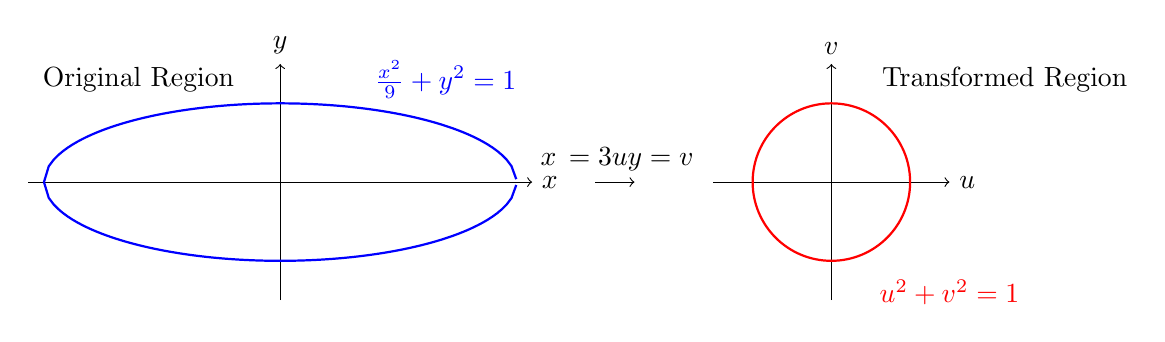
\begin{tikzpicture}[scale=1]
    % Left side - Original elliptical region
    \begin{scope}
        \draw[->] (-3.2,0) -- (3.2,0) node[right] {$x$};
        \draw[->] (0,-1.5) -- (0,1.5) node[above] {$y$};
        \draw[blue, thick] plot[domain=-2:2,samples=100] 
            ({1.5*\x},{sqrt(1-(\x*\x)/4)});
        \draw[blue, thick] plot[domain=-2:2,samples=100] 
            ({1.5*\x},{-sqrt(1-(\x*\x)/4)});
        \node at (-1.8,1.3) {Original Region};
        \node[blue] at (2.1,1.3) {$\frac{x^2}{9} + y^2 = 1$};
    \end{scope}
    
    % Arrow showing transformation
    \draw[->] (4,0) -- (4.5,0) node[midway,above] {$\begin{matrix}x=3u\\y=v\end{matrix}$};
    
    % Right side - Transformed circular region
    \begin{scope}[xshift=7cm]
        \draw[->] (-1.5,0) -- (1.5,0) node[right] {$u$};
        \draw[->] (0,-1.5) -- (0,1.5) node[above] {$v$};
        \draw[red, thick] (0,0) circle (1);
        \node at (2.2,1.3) {Transformed Region};
        \node[red] at (1.5,-1.4) {$u^2 + v^2 = 1$};
    \end{scope}
\end{tikzpicture}
\caption{\textit{Transforming an elliptical region $\frac{x^2}{9} + y^2 = 1$ into a unit circle $u^2 + v^2 = 1$ using the transformation $x = 3u$, $y = v$. The Jacobian determinant $|J| = 3$ accounts for the area scaling.}}
\label{fig:transform} 
\end{figure}

\noindent When applying these transformations, verify that:
\begin{itemize}
    \item The boundary equations simplify in the new coordinates
    \item The Jacobian determinant is nonzero in your region
    \item The transformed region has simpler bounds for integration
\end{itemize}

\subsubsection*{Conditions for Valid Transformations}

\noindent Not every transformation that simplifies our region or integrand is valid for change of variables. For the formula to work, our transformation must be:
\begin{itemize}
    \item One-to-one (each point in $R$ corresponds to exactly one point in $R'$)
    \item Continuously differentiable (all partial derivatives exist and are continuous)
    \item Have a nonzero Jacobian determinant throughout the region
\end{itemize}

\noindent These conditions ensure our transformation preserves the essential structure of the region and allows us to meaningfully compute the transformed integral. They also guarantee that our transformation has an inverse, allowing us to map back to our original coordinates if needed. \\

\noindent The nonzero Jacobian condition is particularly important—it ensures our transformation doesn't ``collapse" any part of the region, which would make the transformation fail to be one-to-one. This explains why polar coordinates have a singularity at the origin (where $r = 0$ and the Jacobian vanishes) and why we must handle such points carefully.

\exampleline
\begin{example}
Consider the integral $\iint_R (x+y)^2\,dx\,dy$ where $R$ is the parallelogram with vertices at $(0,0)$, $(2,0)$, $(1,2)$, and $(3,2)$. Use a linear transformation to convert this to an integral over a rectangle.

\begin{solution}
First, let's understand how to find an appropriate transformation. Looking at our parallelogram:

\begin{figure}[H]
\centering
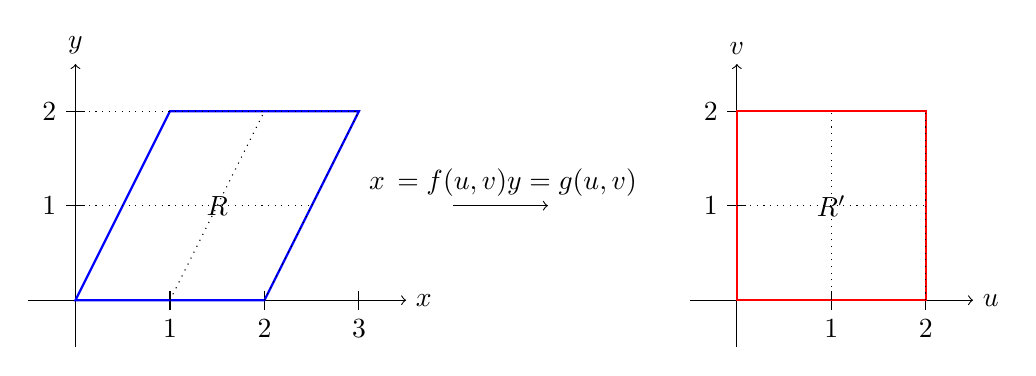
\begin{tikzpicture}[scale=1.2]
   % Original parallelogram
   \begin{scope}
       \draw[->] (-0.5,0) -- (3.5,0) node[right] {$x$};
       \draw[->] (0,-0.5) -- (0,2.5) node[above] {$y$};
       
       % Add coordinate ticks
       \foreach \x in {1,2,3} {
           \draw (\x,0.1) -- (\x,-0.1) node[below] {$\x$};
       }
       \foreach \y in {1,2} {
           \draw (0.1,\y) -- (-0.1,\y) node[left] {$\y$};
       }
       
       \draw[blue, thick] (0,0) -- (2,0) -- (3,2) -- (1,2) -- cycle;
       \node at (1.5,1) {$R$};

       % Add grid to show shearing
       \draw[dotted] (1,0) -- (2,2);
       \draw[dotted] (2,0) -- (3,2);
       \draw[dotted] (0,1) -- (2.5,1);
       \draw[dotted] (0,2) -- (3,2);
   \end{scope}
   
   % Arrow showing transformation
   \draw[->] (4,1) -- (5,1) node[midway,above] {$\begin{matrix}x=f(u,v)\\y=g(u,v)\end{matrix}$};
   
   % Transformed rectangle
   \begin{scope}[xshift=7cm]
       \draw[->] (-0.5,0) -- (2.5,0) node[right] {$u$};
       \draw[->] (0,-0.5) -- (0,2.5) node[above] {$v$};
       
       % Add coordinate ticks
       \foreach \x in {1,2} {
           \draw (\x,0.1) -- (\x,-0.1) node[below] {$\x$};
       }
       \foreach \y in {1,2} {
           \draw (0.1,\y) -- (-0.1,\y) node[left] {$\y$};
       }
       
       \draw[red, thick] (0,0) -- (2,0) -- (2,2) -- (0,2) -- cycle;
       \node at (1,1) {$R'$};
       
       % Add grid to show rectangular nature
       \draw[dotted] (1,0) -- (1,2);
       \draw[dotted] (2,0) -- (2,2);
       \draw[dotted] (0,1) -- (2,1);
   \end{scope}
\end{tikzpicture}
\caption{\textit{We seek a transformation $x = f(u,v)$, $y = g(u,v)$ that ``un-shears" the parallelogram into a rectangle by shifting each horizontal slice back by an amount proportional to its height.}}
\end{figure}

\noindent To find our transformation, we observe that each horizontal line in our parallelogram is shifted right as we move up. Specifically:
\begin{itemize}
    \item At $y = 0$, the line segment goes from $x = 0$ to $x = 2$
    \item At $y = 2$, the line segment goes from $x = 1$ to $x = 3$
\end{itemize}

\noindent This suggests each horizontal line is shifted right by half its height. To undo this shift, we need to subtract $\frac{y}{2}$ from each $x$-coordinate. Therefore, if we let:
\begin{align*}
u &= x - \frac{y}{2} \\
y &= v
\end{align*}

\noindent Solving for $x$ and $y$ gives our transformation:
\begin{align*}
x &= u + \frac{v}{2} \\
y &= v
\end{align*}

\noindent This transformation maps the parallelogram to a rectangle with vertices at $(0,0)$, $(2,0)$, $(0,2)$, and $(2,2)$. To verify this:
\begin{itemize}
    \item When $(u,v) = (0,0)$: $(x,y) = (0,0)$
    \item When $(u,v) = (2,0)$: $(x,y) = (2,0)$
    \item When $(u,v) = (0,2)$: $(x,y) = (1,2)$
    \item When $(u,v) = (2,2)$: $(x,y) = (3,2)$
\end{itemize}

\noindent The Jacobian matrix for this transformation is:
\[
J = \begin{bmatrix}
\frac{\partial x}{\partial u} & \frac{\partial x}{\partial v} \\[1ex]
\frac{\partial y}{\partial u} & \frac{\partial y}{\partial v}
\end{bmatrix} = \begin{bmatrix}
1 & \frac{1}{2} \\
0 & 1
\end{bmatrix}
\]

\noindent Therefore:
\[
|J| = \det\begin{bmatrix}
1 & \frac{1}{2} \\
0 & 1
\end{bmatrix} = 1
\]

\noindent The integrand becomes:
\[
(x+y)^2 = (u + \frac{v}{2} + v)^2 = (u + \frac{3v}{2})^2
\]

\noindent Thus our transformed integral is:
\begin{align*}
\iint_R (x+y)^2\,dx\,dy &= \iint_{R'} (u + \frac{3v}{2})^2\cdot 1\,du\,dv \\
&= \int_0^2\int_0^2 (u + \frac{3v}{2})^2\,du\,dv \\
&= \int_0^2\int_0^2 (u^2 + 3uv + \frac{9v^2}{4})\,du\,dv \\
&= \int_0^2 \left[\frac{u^3}{3} + \frac{3u^2v}{2} + \frac{9v^2u}{4}\right]_0^2\,dv \\
&= \int_0^2 (\frac{8}{3} + 6v + \frac{9v^2}{2})\,dv \\
&= \left[\frac{8v}{3} + 3v^2 + \frac{3v^3}{2}\right]_0^2 \\
&= \frac{16}{3} + 12 + 12 = \frac{88}{3}
\end{align*}

\noindent Note that $|J| = 1$ made this transformation particularly nice, as we didn't need to multiply by any extra factors. The transformation simplified our region (making it rectangular) while keeping the integrand relatively manageable.
\end{solution}
\end{example}
\exampleline

\begin{example}
An astronomer is studying the density of a spiral galaxy. The density at any point is given by 
\[
\rho(x,y) = e^{-\left(\frac{x^2}{4} + y^2\right)} e^{-\tan^{-1}\left(\frac{2y}{x}\right)}
\]
where \((x,y)\) represents the position in kiloparsecs from the galactic center. Find the total mass contained within the elliptical region bounded by \(\frac{x^2}{4} + y^2 = 1\) using appropriate changes of variables.

\begin{solution}
\noindent Let's first understand our region of integration. We have an ellipse defined by \(\frac{x^2}{4} + y^2 = 1\). To simplify the integration, we'll transform this ellipse into a unit circle through a change of variables. Ellipse to circle transformations are not too hard. We just need to make the coefficient on $x^2$ to be $1$ and transform $y$ to $v$.\\

\noindent Consider the linear transformation:
\begin{align*}
x &= 2u \\
y &= v
\end{align*}

\noindent We will have the same sort of region transformation as seen in Figure \ref{fig:transform}. When we substitute these into the equation of our ellipse:
\[
\frac{(2u)^2}{4} + v^2 = \frac{4u^2}{4} + v^2 = u^2 + v^2 = 1
\]
we verify that our elliptical region transforms into the unit circle \(u^2 + v^2 = 1\).

\noindent The Jacobian matrix for this transformation is:
\[
J = \begin{bmatrix}
\frac{\partial x}{\partial u} & \frac{\partial x}{\partial v} \\[1ex]
\frac{\partial y}{\partial u} & \frac{\partial y}{\partial v}
\end{bmatrix} = \begin{bmatrix}
2 & 0 \\
0 & 1
\end{bmatrix}
\]

\noindent Therefore, \(|J| = 2\). Under this transformation, the density function becomes:
\[
\rho(u,v) = e^{-(u^2 + v^2)} e^{-\tan^{-1}\left(\frac{v}{u}\right)}
\]

\noindent To further simplify integration over the unit circle, we can use polar coordinates:
\begin{align*}
u &= r\cos\theta \\
v &= r\sin\theta
\end{align*}

\noindent The Jacobian for this polar transformation is \(r\). Substituting these into our density function:
\[
\rho(r,\theta) = e^{-r^2} e^{-\theta}
\]

\noindent Combining both changes of variables with their respective Jacobians, our mass integral becomes:
\[
M = 2 \int_0^{2\pi} \int_0^1 e^{-r^2} e^{-\theta} r \, dr \, d\theta
\]

\noindent This integral is set up in a way that separates the variables, potentially simplifying evaluation:
\[
M = 2 \left( \int_0^{2\pi} e^{-\theta} \, d\theta \right) \left( \int_0^1 e^{-r^2} r \, dr \right)
\]

\noindent While the integral over \(r\) can be evaluated using substitution, the integral over \(\theta\) is straightforward:
\[
\int_0^{2\pi} e^{-\theta} \, d\theta = \left[ -e^{-\theta} \right]_0^{2\pi} = -(e^{-2\pi} - 1) = 1 - e^{-2\pi}
\]

\noindent The integral over \(r\) can be evaluated using substitution \(w = r^2\), \(dw = 2r\,dr\):
\[
\int_0^1 e^{-r^2} r \, dr = \frac{1}{2} \int_0^1 e^{-w} \, dw = \frac{1}{2} \left[ -e^{-w} \right]_0^1 = \frac{1}{2} (1 - e^{-1})
\]

\noindent Therefore, the total mass is:
\[
M = 2 \left(1 - e^{-2\pi}\right) \left( \frac{1}{2} \left(1 - e^{-1}\right) \right) = \left(1 - e^{-2\pi}\right) \left(1 - e^{-1}\right)
\]
\end{solution}
\end{example}
\exampleline




\newpage

\lecture{Applications of Triple Integrals}

\noindent Having developed the machinery for evaluating triple integrals in various coordinate systems, we now explore how these tools illuminate real-world physical phenomena. Just as double integrals helped us analyze flat objects with varying properties, triple integrals allow us to study three-dimensional bodies and their characteristics. The applications we'll encounter demonstrate how calculus provides precise mathematical descriptions of physical reality.

\subsection*{Mass and Density in Three Dimensions} \index{Mass and Density}

\noindent Consider a solid object occupying a region $E$ in space. Like we described in Lecture 3 of this chapter, real materials often have density that varies from point to point. A wooden beam might have varying density due to its grain structure; a block of metal might have impurities or intentional composition gradients; even the atmosphere has density that changes with altitude. We can represent this variation using a density function $\rho(x,y,z)$ that gives the mass per unit volume at each point. \\

\noindent To find the total mass of such an object, we follow the same reasoning that led us to double integrals: we partition our region into small volume elements, multiply each element's volume by its density, and sum over all elements. In the limit, this process yields:
\[
M = \iiint_E \rho(x,y,z)\,dV
\]

\noindent This integral emerges naturally from the physical principle that mass is additive—the total mass is the sum of the masses of all small pieces. Each infinitesimal piece has volume $dV$ and density $\rho(x,y,z)$, giving it mass $\rho(x,y,z)\,dV$. The triple integral then sums these contributions over the entire region.

\subsubsection*{Center of Mass and Balance} \index{Center of Mass}

\noindent Just as with flat plates, understanding where a three-dimensional object balances is crucial for engineering applications. The center of mass of a solid object tells us where it effectively balances and how it will behave when rotating. For an object with density $\rho(x,y,z)$, we find its center of mass coordinates $(\bar{x}, \bar{y}, \bar{z})$ using:
\begin{align*}
\bar{x} &= \frac{1}{M}\iiint_E x\rho(x,y,z)\,dV \\
\bar{y} &= \frac{1}{M}\iiint_E y\rho(x,y,z)\,dV \\
\bar{z} &= \frac{1}{M}\iiint_E z\rho(x,y,z)\,dV
\end{align*}

\noindent These formulas arise from the physical principle of torque balance. Each point in the object creates a torque proportional to both its mass and its distance from the axis. The numerator integrals sum up these torque contributions, while division by the total mass $M$ gives us the balancing point. This generalizes our earlier work with double integrals to fully three-dimensional scenarios.

%https://commons.wikimedia.org/wiki/File:Bird_toy_showing_center_of_gravity.jpg
\begin{figure}[H]
\centering
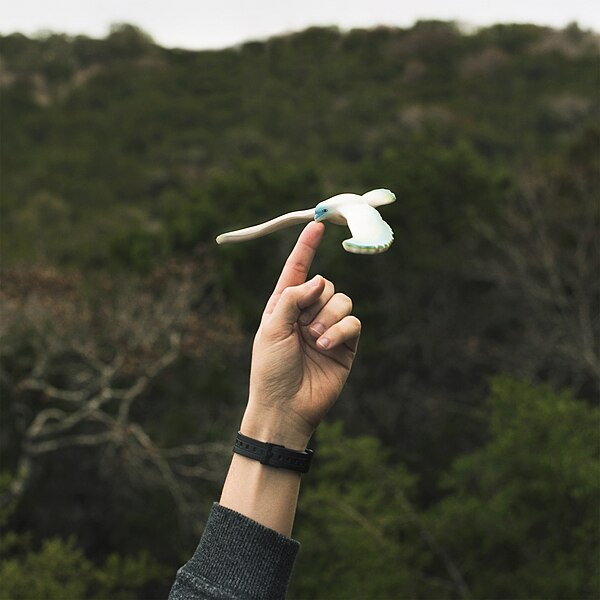
\includegraphics[width=0.4\textwidth]{chapters/chp4_pics/COG.jpg}
\caption{\textit{A balancing bird toy demonstrates the principle of center of mass. While often called the center of gravity, these terms are equivalent on Earth where gravitational field strength is approximately uniform. The bird's center of mass is carefully positioned below its support point (the beak) via a non-uniform density throughout the toy, creating a stable equilibrium. When disturbed, the bird will oscillate around this equilibrium point until returning to its stable position—a principle fundamental to both engineering design and physical analysis.}}
\label{fig:balance_bird}
\end{figure}


\exampleline
\begin{example}
A metal foundry is producing a cylindrical rod with a height of $L = 1$ meter and a radius of $R = 0.5$ meters. Due to the cooling process, the density of the rod varies with height according to $\rho(x,y,z) = k z^2$, where $z$ measures the height from the base of the cylinder. The total mass of the rod is measured to be $M = 10$ kg.

\begin{enumerate}
    \item Determine the value of the constant $k$ that describes the density distribution.
    \item Calculate the $z$-coordinate of the center of mass of the rod from the base.
\end{enumerate}

\begin{solution}
\begin{enumerate}
    \item \textbf{Determine $k$}: 

    The total mass of the rod is given by:
    \[
    M = \iiint_E \rho(x,y,z)\,dV.
    \]
    In cylindrical coordinates, $x^2 + y^2 = r^2$, and $dV = r\,dr\,d\theta\,dz$. The density becomes $\rho(r,\theta,z) = k z^2$, and the region $E$ is defined by $r \in [0, R]$, $\theta \in [0, 2\pi]$, and $z \in [0, L]$. Substituting:
    \[
    M = \int_0^L \int_0^{2\pi} \int_0^R k z^2 r \,dr\,d\theta\,dz.
    \]
    Separate the integrals:
    \[
    M = k \int_0^L z^2\,dz \int_0^{2\pi} d\theta \int_0^R r\,dr.
    \]
    Compute each integral:
    \[
    \int_0^{2\pi} d\theta = 2\pi, \quad \int_0^R r\,dr = \left[\frac{r^2}{2}\right]_0^R = \frac{R^2}{2}, \quad \int_0^L z^2\,dz = \left[\frac{z^3}{3}\right]_0^L = \frac{L^3}{3}.
    \]
    Substitute into the equation for $M$:
    \[
    M = k \cdot \frac{L^3}{3} \cdot 2\pi \cdot \frac{R^2}{2}.
    \]
    Simplify:
    \[
    M = k \cdot \frac{\pi R^2 L^3}{3}.
    \]
    Solve for $k$:
    \[
    k = \frac{3M}{\pi R^2 L^3}.
    \]
    Substitute $M = 10$, $R = 0.5$, and $L = 1$:
    \[
    k = \frac{3 \cdot 10}{\pi \cdot (0.5)^2 \cdot 1^3} = \frac{30}{\pi \cdot 0.25} = \frac{120}{\pi}.
    \]

    \item \textbf{Find the center of mass}: 

    The $z$-coordinate of the center of mass is:
    \[
    \bar{z} = \frac{1}{M} \iiint_E z \rho(x,y,z)\,dV.
    \]
    In cylindrical coordinates:
    \[
    \bar{z} = \frac{1}{M} \int_0^L \int_0^{2\pi} \int_0^R z (k z^2) r \,dr\,d\theta\,dz.
    \]
    Separate the integrals:
    \[
    \bar{z} = \frac{k}{M} \int_0^L z^3\,dz \int_0^{2\pi} d\theta \int_0^R r\,dr.
    \]
    Compute each integral:
    \[
    \int_0^{2\pi} d\theta = 2\pi, \quad \int_0^R r\,dr = \frac{R^2}{2}, \quad \int_0^L z^3\,dz = \left[\frac{z^4}{4}\right]_0^L = \frac{L^4}{4}.
    \]
    Substitute:
    \[
    \bar{z} = \frac{k}{M} \cdot \frac{L^4}{4} \cdot 2\pi \cdot \frac{R^2}{2}.
    \]
    Simplify:
    \[
    \bar{z} = \frac{k \pi R^2 L^4}{4M}.
    \]
    Substituting $k = \frac{120}{\pi}$, $M = 10$, $R = 0.5$, and $L = 1$:
    \[
    \bar{z} = \frac{\frac{120}{\pi} \cdot \pi \cdot (0.5)^2 \cdot 1^4}{4 \cdot 10}.
    \]
    Simplify:
    \[
    \bar{z} = \frac{120 \cdot 0.25}{40} = \frac{30}{40} = 0.75 \, \text{meters}.
    \]

    \noindent The center of mass of the rod is located $0.75$ meters from the base.
\end{enumerate}
\end{solution}
\end{example}
\exampleline


\subsection*{Moments and Products of Inertia in Three Dimensions} \index{Moment of Inertia} \index{Product of Inertia}

\noindent When an object rotates, its resistance to changes in rotational motion depends not just on its total mass but on how that mass is distributed. Think of a figure skater pulling in their arms to spin faster, or a diver tucking into a ball to increase their rotation speed. These effects are described by quantities called moments and products of inertia. \\

\noindent For rotation about the coordinate axes, we define the moments of inertia:
\begin{align*}
I_x &= \iiint_E (y^2 + z^2)\rho(x,y,z)\,dV \\
I_y &= \iiint_E (x^2 + z^2)\rho(x,y,z)\,dV \\
I_z &= \iiint_E (x^2 + y^2)\rho(x,y,z)\,dV
\end{align*}

\noindent Each moment measures how hard it is to rotate the object about that axis. Notice the squared terms - mass farther from the axis contributes more to the moment of inertia, just as it's harder to spin a dumbbell held at arm's length than one held close to your body. \\

\noindent The products of inertia capture how rotation about one axis affects rotation about others:
\begin{align*}
I_{xy} &= \iiint_E xy\rho(x,y,z)\,dV \\
I_{yz} &= \iiint_E yz\rho(x,y,z)\,dV \\
I_{xz} &= \iiint_E xz\rho(x,y,z)\,dV
\end{align*}
\index{Tensors}
\noindent This distribution is characterized by moments and products of inertia that we can arrange in a special $3 \times 3$ grid called the inertia tensor:
\[
\begin{bmatrix}
I_{xx} & -I_{xy} & -I_{xz} \\
-I_{yx} & I_{yy} & -I_{yz} \\
-I_{zx} & -I_{zy} & I_{zz}
\end{bmatrix}
\]

\noindent Though this appears as a matrix (a 2-dimensional array of numbers), it represents something more fundamental in physics. Just as vectors (1-dimensional arrays) are special cases of matrices, matrices themselves are special cases of tensors - mathematical objects that preserve relationships between physical quantities regardless of how we measure them. Consider a spinning top - its rotational behavior remains the same whether we measure it using $xyz$ coordinates or any other system. The inertia tensor $\mathbf{I}$ captures this fundamental behavior by relating angular velocity to angular momentum in a way that remains true under any coordinate transformation. While the mathematics of tensors extends beyond this text, we can work with $\mathbf{I}$ as a matrix while appreciating its deeper physical significance. \\

\noindent This structure explains why there exist three special directions called principal axes where rotation is simplest - imagine spinning a book along its length, width, or thickness. When rotating about these axes, the object spins cleanly without wobbling. While finding these directions involves concepts from linear algebra that we'll encounter in later courses, understanding their existence helps explain why gymnasts and divers choose particular axes for their rotations.\\

\noindent These physical insights manifest in several fundamental equations. For any rotating object in 3D space, with angular velocity $\boldsymbol{\omega} = (\omega_x, \omega_y, \omega_z)$ and angular acceleration $\boldsymbol{\alpha} = (\alpha_x, \alpha_y, \alpha_z)$, we can describe its motion using the inertia tensor:

\begin{itemize} \index{Angular Momentum}
   \item Angular momentum:
   \[
   \begin{bmatrix} L_x \\ L_y \\ L_z \end{bmatrix} = 
   \begin{bmatrix}
   I_{xx} & -I_{xy} & -I_{xz} \\
   -I_{yx} & I_{yy} & -I_{yz} \\
   -I_{zx} & -I_{zy} & I_{zz}
   \end{bmatrix}
   \begin{bmatrix} \omega_x \\ \omega_y \\ \omega_z \end{bmatrix}
   \]
   
   \item Rotational kinetic energy: \index{Rotational Motion}
   \[
   E = \frac{1}{2}\begin{bmatrix} \omega_x & \omega_y & \omega_z \end{bmatrix}
   \begin{bmatrix}
   I_{xx} & -I_{xy} & -I_{xz} \\
   -I_{yx} & I_{yy} & -I_{yz} \\
   -I_{zx} & -I_{zy} & I_{zz}
   \end{bmatrix}
   \begin{bmatrix} \omega_x \\ \omega_y \\ \omega_z \end{bmatrix}
   \]
   
   \item Torque: \index{Torque}
   \[
   \begin{bmatrix} \tau_x \\ \tau_y \\ \tau_z \end{bmatrix} = 
   \begin{bmatrix}
   I_{xx} & -I_{xy} & -I_{xz} \\
   -I_{yx} & I_{yy} & -I_{yz} \\
   -I_{zx} & -I_{zy} & I_{zz}
   \end{bmatrix}
   \begin{bmatrix} \alpha_x \\ \alpha_y \\ \alpha_z \end{bmatrix}
   \]
\end{itemize}

\noindent When an object is symmetric or rotates about a principal axis, the off-diagonal terms ($I_{xy}, I_{yz}, I_{xz}$) become zero and these equations simplify to the scalar forms seen earlier. Common examples include a cylinder spinning about its axis or a sphere rotating about any diameter. \\

\noindent These matrix operations work as follows: \\

\noindent \textbf{Matrix-Vector Multiplication:} \index{Matrix Operations} When multiplying a $3 \times 3$ matrix by a $3 \times 1$ vector:
\[
\begin{bmatrix}
a & b & c \\
d & e & f \\
g & h & i
\end{bmatrix}
\begin{bmatrix}
x \\ y \\ z
\end{bmatrix}
=
\begin{bmatrix}
ax + by + cz \\
dx + ey + fz \\
gx + hy + iz
\end{bmatrix}
\]

\noindent \textbf{Vector-Matrix-Vector Multiplication:} For a row vector times matrix times column vector:
\[
\begin{bmatrix} x & y & z \end{bmatrix}
\begin{bmatrix}
a & b & c \\
d & e & f \\
g & h & i
\end{bmatrix}
\begin{bmatrix} x \\ y \\ z \end{bmatrix}
= ax^2 + (b+d)xy + (c+g)xz + (e)y^2 + (f+h)yz + (i)z^2
\]

\noindent This explains why the kinetic energy expression $E = \frac{1}{2}\boldsymbol{\omega}^T\mathbf{I}\boldsymbol{\omega}$ produces a scalar value - it's a vector-matrix-vector product that combines all the moments and products of inertia with the angular velocity components. The $T$ over $\boldsymbol{\omega}$ represents the \textit{transpose} which switches the component indices, i.e., $x_{ij}$ becomes $x_{ji}$. Note that this can also change the structure, especially seen in the kinetic energy expression where the dimensions of $\boldsymbol{\omega}$ are $3 \times 1$ where $\boldsymbol{\omega}^T$ has dimensions $1 \times 3$ which are not the same and have different structural meanings.

%https://commons.wikimedia.org/wiki/File:Matrix_multiplication_qtl1.svg
\begin{figure}[H]
\centering
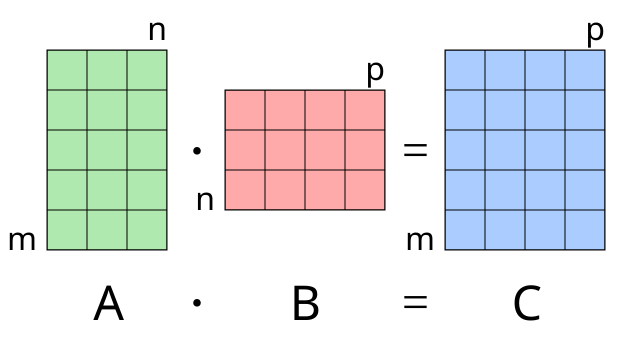
\includegraphics[width=0.4\textwidth]{chapters/chp4_pics/matrix.png}
\caption{\textit{A visualization of matrix operations. Notice the change in dimensionality. For any matrix multiplication we will have $A_{m\times n} \cdot B_{n \times p} = C_{m \times p}$. Note that the column dimension of $A$ must equal the row dimension of $B$ or else you cannot perform the matrix operation}}
\label{fig:matrix}
\end{figure}

\noindent Matrices naturally emerge in multivariate calculus as they elegantly encode how quantities in multiple dimensions relate to and transform each other, just as we've seen with moments of inertia describing rotational motion. While we've only scratched the surface here, a deeper study of linear algebra reveals powerful tools for understanding everything from coordinate transformations to optimization problems in higher dimensions. As you continue your mathematical journey, we strongly encourage exploring linear algebra to gain deeper insight into the beautiful structures underlying multivariate calculus.

\subsection*{Force and Work in Space}

\noindent When a force varies continuously throughout a region of space, triple integrals help us calculate its effects. Consider a force field $\mathbf{F}(x,y,z)$ acting on a solid object. Just as with mass distribution, we can integrate the components of the force field over the region to find the total force exerted on the object in each direction:
\begin{align*}
F_x &= \iiint_E F_x(x,y,z)\,dV, \\
F_y &= \iiint_E F_y(x,y,z)\,dV, \\
F_z &= \iiint_E F_z(x,y,z)\,dV.
\end{align*}

\noindent Work---the energy transferred by a force acting over a displacement---is most naturally computed along a specific path using a \textit{line integral}, which we will develop fully in Chapter 5. For now, we focus on what triple integrals \textit{can} tell us: the \textbf{total instantaneous power} exerted on a distributed body.\\ \\
\noindent When a force field \( \mathbf{F}(x,y,z) \) acts on a body whose points move with velocity field \( \mathbf{v}(x,y,z) \), the \textit{power density} (rate of doing work per unit volume) at each point is:
\[
P(x,y,z) = \mathbf{F}(x,y,z) \cdot \mathbf{v}(x,y,z).
\]
The total instantaneous power delivered to the body is then:
\[
\mathcal{P}_{\text{total}} = \iiint_E \mathbf{F}(x,y,z) \cdot \mathbf{v}(x,y,z) \, dV.
\]
\noindent To find the actual \textit{work} (energy) delivered over a time interval, one would integrate the total power over time: \( W = \int_0^T \mathcal{P}_{\text{total}}(t) \, dt \). We will see more direct approaches to computing work in Chapter 5.

\noindent This framework is essential in physics and engineering applications. For example, when calculating the work done by an electric field $\mathbf{E}$ on a charge distribution $\rho(x,y,z)$ moving with velocity $\mathbf{v}(x,y,z)$, the integral takes the form:
\[
W = \iiint_E \rho(x,y,z)\bigl(\mathbf{E} \cdot \mathbf{v}\bigr)\,dV,
\]
where $\mathbf{v}$ is the local velocity vector at each point in the charge distribution. Here, the triple integral sums contributions to the total work throughout the entire region of charge. This process models how electric forces interact with volumetric charge distributions in systems such as capacitors or plasma clouds. \\

\noindent In Chapter 5, we will refine these concepts further by introducing line integrals and exploring how work is more directly computed along specific paths within a vector field. For now, understand that triple integrals are invaluable for modeling distributed forces and power densities across volumes.

\exampleline
\begin{example}
A magnetic field $\mathbf{B}(x,y,z) = (y^2, xz, xy)$ tesla acts on a conductive fluid in the unit cube $[0,1]^3$. The fluid has charge density $\rho(x,y,z) = e^{-(x^2 + y^2 + z^2)}  \text{(coulombs/m$^3$)}$ and velocity $\mathbf{v}(x,y,z) = (z, x, y) \quad \text{(m/s)}$. \\

\noindent Find:
\begin{enumerate}
   \item The total magnetic force on the fluid given the differential Lorentz force $d\mathbf{F} =  \rho(\mathbf{r}) \bigl(\mathbf{v} \times \mathbf{B}\bigr)\,dV$ and force density $\mathbf{f}(\mathbf{r}) = \rho(\mathbf{r})\,[\,\mathbf{v}(\mathbf{r}) \times \mathbf{B}(\mathbf{r})\,]$
   \item The work done by the magnetic field in one second, given that instantaneous power is $dP = \mathbf{F}\cdot\mathbf{v}$
\end{enumerate}

\begin{solution}
\begin{enumerate}
   \item \textbf{Total Magnetic Force on the Fluid} \\
   
   Computing the cross product:
   \[
   \mathbf{v} \times \mathbf{B}
   =
   \begin{vmatrix}
   \mathbf{i} & \mathbf{j} & \mathbf{k}\\
   z & x & y\\
   y^2 & xz & xy
   \end{vmatrix}
   =
   \bigl(x^2y - xyz,\;\;y^3 - xyz,\;\;xz^2 - xy^2\bigr)
   \]
   
   Hence the total force components are:
   \begin{align*}
   F_x &= \iiint_{E=[0,1]^3} e^{-(x^2 + y^2 + z^2)}\,(x^2y - x y z)\, dV \\[1ex]
   F_y &= \iiint_{E=[0,1]^3} e^{-(x^2 + y^2 + z^2)}\,(y^3 - x y z)\, dV \\[1ex]
   F_z &= \iiint_{E=[0,1]^3} e^{-(x^2 + y^2 + z^2)}\,(x z^2 - x y^2)\, dV
   \end{align*}

   \item \textbf{Work Done by the Magnetic Field in One Second} \\
   
   For a fluid element, the differential power is:
   \[
   dP = \bigl[\rho(\mathbf{v}\times\mathbf{B})\bigr]\cdot\mathbf{v}\,dV 
   \;=\; \rho \bigl(\mathbf{v}\times\mathbf{B}\bigr)\cdot \mathbf{v}\, dV
   \]
   
   Because $\mathbf{v}\times\mathbf{B}$ is always perpendicular to $\mathbf{v}$, their dot product is zero:
   \[
   (\mathbf{v}\times\mathbf{B})\cdot\mathbf{v} = 0
   \]
   
   Thus the magnetic field does no work on the fluid:
   \[
   W = \iiint_{E} \rho \bigl[(\mathbf{v}\times\mathbf{B})\cdot\mathbf{v}\bigr]\; dV = 0
   \]
\end{enumerate}

\end{solution}
\end{example}
\exampleline
\begin{example}
A force field $\mathbf{F}(x,y,z) = (yz, xz, xy)$ newtons acts on a volume of gas expanding in the unit cube $[0,1]^3$. The gas particles move with velocity
\[
\mathbf{v}(x,y,z) = (x, y, z) \quad \text{(m/s)}.
\]
Find:
\begin{enumerate}
   \item The total force on the gas volume
   \item The work done by the force field on the gas, given that instantaneous power is $dP = \mathbf{F}\cdot\mathbf{v}\,dV$
\end{enumerate}

\begin{solution}
\begin{enumerate}
   \item \textbf{Total Force Components} \\
   
   The total force is found by integrating each component over the volume:
   \begin{align*}
   F_x &= \iiint_{[0,1]^3} yz\,dV = \int_0^1\int_0^1\int_0^1 yz\,dx\,dy\,dz \\
   &= \int_0^1\int_0^1 yz\,dy\,dz = \int_0^1 \frac{z}{2}\,dz = \frac{1}{4} \\[2ex]
   F_y &= \iiint_{[0,1]^3} xz\,dV = \int_0^1\int_0^1\int_0^1 xz\,dx\,dy\,dz \\
   &= \int_0^1\int_0^1 \frac{z}{2}\,dy\,dz = \frac{1}{4} \\[2ex]
   F_z &= \iiint_{[0,1]^3} xy\,dV = \int_0^1\int_0^1\int_0^1 xy\,dx\,dy\,dz \\
   &= \int_0^1\int_0^1 \frac{y}{2}\,dy\,dz = \frac{1}{4}
   \end{align*}
   
   Therefore $\mathbf{F}_{total} = (\frac{1}{4}, \frac{1}{4}, \frac{1}{4})$ newtons.

   \item \textbf{Work Done by the Force Field} \\
   
   The instantaneous power at each point is:
   \begin{align*}
   \mathbf{F}\cdot\mathbf{v} &= (yz, xz, xy)\cdot(x, y, z) \\
   &= xyz + xyz + xyz \\
   &= 3xyz
   \end{align*}
   
   Therefore the total work done is:
   \begin{align*}
   W &= \iiint_{[0,1]^3} 3xyz\,dV \\
   &= 3\int_0^1\int_0^1\int_0^1 xyz\,dx\,dy\,dz \\
   &= 3\int_0^1\int_0^1 \frac{y}{2}z\,dy\,dz \\
   &= 3\int_0^1 \frac{z}{4}\,dz = \frac{3}{8} \text{ joules}
   \end{align*}
\end{enumerate}
\end{solution}
\end{example}
\exampleline

\subsection*{Average Values and Distributions} \index{Average Value} \index{Average Distribution}

\noindent Just as we found average values using double integrals, we can find the average value of a function $f(x,y,z)$ over a three-dimensional region $E$:
\[
f_{avg} = \frac{\iiint_E f(x,y,z)\,dV}{\iiint_E dV}
\]

\noindent This concept proves invaluable in various physical contexts:
\begin{itemize}
\item Temperature distribution in a solid body, where $f(x,y,z)$ represents temperature
\item Concentration of a solute in a solution, where $f(x,y,z)$ gives concentration
\item Stress distribution in a structural element, where $f(x,y,z)$ describes stress intensity
\end{itemize}

\noindent The denominator $\iiint_E dV$ represents the volume of region $E$, making this formula a natural extension of the average value theorem to three dimensions. When working with non-uniform materials, we often need weighted averages that account for varying density:
\[
f_{avg} = \frac{\iiint_E f(x,y,z)\rho(x,y,z)\,dV}{\iiint_E \rho(x,y,z)\,dV}
\]

\noindent This weighted form finds particular use in materials science and engineering, where we might need to account for how material properties vary throughout a component. For instance, in a composite material, both density and thermal conductivity might vary spatially, affecting the overall thermal behavior of the object.


\exampleline
\begin{example}
A spherical blast furnace of radius 3 meters operates at extremely high temperatures. The temperature (in Celsius) at any point $(x,y,z)$ in the furnace varies according to:
\[
T(x,y,z) = 1500e^{-(x^2+y^2+z^2)/9} + 500
\]
The density of the gas inside the furnace varies with height according to:
\[
\rho(x,y,z) = e^{-z/3} \quad \text{(kg/m}^3\text{)}
\]
Find:
\begin{enumerate}
   \item The average temperature in the furnace
   \item The density-weighted average temperature, accounting for the fact that hotter regions tend to have different densities
\end{enumerate}

\begin{solution}
\begin{enumerate}
   \item First, note the volume of our region $E$, a sphere of radius 3:
   \[
   \iiint_E dV = \frac{4}{3}\pi(3^3) = 36\pi
   \]
   The average temperature is:
   \[
   T_{\mathrm{avg}} = \frac{\iiint_E T(x,y,z)\,dV}{\iiint_E dV} = \frac{\iiint_E T(x,y,z)\,dV}{36\pi}
   \]
   Converting to spherical coordinates $\bigl(r,\phi,\theta\bigr)$ with 
   \[
   x = r\sin\phi\cos\theta,\quad
   y = r\sin\phi\sin\theta,\quad
   z = r\cos\phi,\quad
   dV = r^2\sin\phi\,dr\,d\phi\,d\theta,
   \]
   we have $x^2 + y^2 + z^2 = r^2$, so the temperature becomes
   \[
   T(r) = 1500\,e^{-\tfrac{r^2}{9}} + 500.
   \]
   Therefore,
   \[
   \iiint_E T(x,y,z)\,dV 
   = \int_0^{2\pi}\!\int_0^{\pi}\!\int_0^3 \Bigl(1500\,e^{-\tfrac{r^2}{9}} + 500\Bigr)\,r^2\sin\phi\,dr\,d\phi\,d\theta.
   \]
   The angular parts give a factor of $4\pi$, so
   \[
   \iiint_E T(x,y,z)\,dV 
   = 4\pi\Bigl[
      1500\int_0^3 r^2 e^{-\tfrac{r^2}{9}}\,dr
      + 500\int_0^3 r^2\,dr
   \Bigr].
   \]
   Evaluating,
   \[
   \int_0^3 r^2\,dr = 9
   \quad\text{and}\quad
   \int_0^3 r^2 e^{-\tfrac{r^2}{9}}\,dr \approx 5.12.
   \]
   Hence,
   \[
   1500 \cdot 5.12 + 500 \cdot 9
   = 7680 + 4500
   = 12180.
   \]
   Multiplying by $4\pi$ gives:
   \[
   12180 \cdot 4\pi = 48720\pi.
   \]
   So
   \[
   T_{\mathrm{avg}} 
   = \frac{48720\pi}{36\pi} 
   \approx 1353\;\text{°C}.
   \]

   \item The density-weighted average temperature is
   \[
   T_{\mathrm{avg}} 
   = \frac{\iiint_E T(x,y,z)\,\rho(x,y,z)\,dV}
          {\iiint_E \rho(x,y,z)\,dV}.
   \]
   In spherical coordinates, $z = r\cos\phi$, so
   \[
   \rho(r,\phi) = e^{-\tfrac{r\cos\phi}{3}}.
   \]
   The resulting integrals involve products of exponentials in $r$ and $\cos\phi$, so we evaluate them numerically using programming or Wolfram Alpha. One finds
   \[
   T_{\mathrm{avg}} \approx 1280\;\text{°C}.
   \]
\end{enumerate}
\vspace{0.5em}
\noindent
The density-weighted average is lower because the hotter central regions (larger $r^2$ term in $e^{-r^2/9}$) coincide with regions where $\rho$ is relatively smaller for higher $z$; effectively, less ``weight” is assigned to the hottest points.
\end{solution}
\end{example}
\exampleline



\newpage

\formsdefs{}

\subsection*{Important Vocabulary}
\begin{itemize}
\item \textbf{Double Integral:} A mathematical tool that measures accumulation over a two-dimensional region, used to find quantities like area, volume, mass, and center of mass.

\item \textbf{Double Integral Type I Region:} A region \(R\) in the \((x,y)\)-plane of the form \(R = \{(x,y) : a \leq x \leq b, g_1(x) \leq y \leq g_2(x)\}\), where vertical lines intersect the region's boundary exactly twice.

\item \textbf{Double Integral Type II Region:} A region \(R\) in the \((x,y)\)-plane of the form \(R = \{(x,y) : c \leq y \leq d, h_1(y) \leq x \leq h_2(y)\}\), where horizontal lines intersect the region's boundary exactly twice.

\item \textbf{Fubini's Theorem:} States that a double or triple integral can be evaluated as repeated integrals in any order over a rectangular region.

\item \textbf{Triple Integral:} An extension of double integrals to three dimensions, used to find volumes, mass, and other physical quantities in \(\mathbb{R}^3\).

\item \textbf{Triple Integral Type I Region:} A solid region \(E\) bounded above and below by surfaces \(z = g_2(x,y)\) and \(z = g_1(x,y)\) over a region \(R\) in the \((x,y)\)-plane, where vertical lines intersect the boundary exactly twice.

\item \textbf{Triple Integral Type II Region:} A solid region \(E\) bounded by surfaces \(x = h_1(y,z)\) and \(x = h_2(y,z)\) over a region \(R\) in the \((y,z)\)-plane, where lines parallel to the \(x\)-axis intersect the boundary exactly twice.

\item \textbf{Triple Integral Type III Region:} A solid region \(E\) bounded by surfaces \(y = k_1(x,z)\) and \(y = k_2(x,z)\) over a region \(R\) in the \((x,z)\)-plane, where lines parallel to the \(y\)-axis intersect the boundary exactly twice.

\item \textbf{Jacobian Determinant:} A measure of how a coordinate transformation affects area or volume elements, denoted \(|J|\).

\item \textbf{Moment of Inertia:} A measure of an object's resistance to rotational motion about an axis, denoted \(I_x\), \(I_y\), or \(I_z\).

\item \textbf{Product of Inertia:} A measure of coupling between rotations about different axes, denoted \(I_{xy}\), \(I_{yz}\), or \(I_{xz}\).

\item \textbf{Center of Mass:} The point \((\bar{x}, \bar{y}, \bar{z})\) where an object's mass can be considered concentrated for certain calculations.

\item \textbf{Inertia Tensor:} A \(3\times3\) matrix describing how mass is distributed in a rotating object.

\item \textbf{Iterated Integral:} A multiple integral evaluated as a sequence of single integrals, integrating one variable at a time while treating the others as constants.

\item \textbf{Polar Coordinates:} A coordinate system \( (r, \theta) \) where \( r \) is the distance from the origin and \( \theta \) is the angle from the positive \( x \)-axis. The area element is \( dA = r \, dr \, d\theta \).

\item \textbf{Cylindrical Coordinates:} A coordinate system \( (r, \theta, z) \) extending polar coordinates by adding a height \( z \). The volume element is \( dV = r \, dr \, d\theta \, dz \).

\item \textbf{Spherical Coordinates:} A coordinate system \( (\rho, \theta, \phi) \) where \( \rho \) is the distance from the origin, \( \theta \) is the azimuthal angle, and \( \phi \) is the polar angle from the \( z \)-axis. The volume element is \( dV = \rho^2 \sin\phi \, d\rho \, d\theta \, d\phi \).

\item \textbf{Change of Variables:} A technique for simplifying integrals by substituting new coordinate variables, requiring multiplication by the absolute value of the Jacobian determinant.

\item \textbf{Surface Area:} The area of a surface \( z = f(x,y) \) over a region \( R \), computed as \( \iint_R \sqrt{1 + f_x^2 + f_y^2} \, dA \).
\end{itemize}

\subsection*{Key Formulas}
\begin{multicols}{2}

\paragraph{Fubini's Theorem (Rectangular)}
\[
\iint_R f\,dA = \int_a^b\!\int_c^d f(x,y)\,dy\,dx = \int_c^d\!\int_a^b f(x,y)\,dx\,dy
\]

\paragraph{Type I Region (vertical slicing)}
\[
\iint_R f\,dA = \int_a^b\!\int_{g_1(x)}^{g_2(x)} f(x,y)\,dy\,dx
\]

\paragraph{Type II Region (horizontal slicing)}
\[
\iint_R f\,dA = \int_c^d\!\int_{h_1(y)}^{h_2(y)} f(x,y)\,dx\,dy
\]

\paragraph{Polar Coordinates}
\begin{align*}
x &= r\cos\theta, \quad y = r\sin\theta \\
dA &= r\,dr\,d\theta
\end{align*}
\[
\iint_R f\,dA = \int_\alpha^\beta\!\int_{r_1(\theta)}^{r_2(\theta)} f(r\cos\theta,r\sin\theta)\,r\,dr\,d\theta
\]

\paragraph{Area and Volume}
\[
\text{Area} = \iint_R 1\,dA \qquad \text{Volume} = \iiint_E 1\,dV
\]

\paragraph{Surface Area ($z = g(x,y)$)}
\[
A = \iint_R \sqrt{1 + g_x^2 + g_y^2}\,dA
\]

\paragraph{Mass, Moments, Center of Mass (2D)}
\begin{align*}
M &= \iint_R \rho\,dA \\
M_x &= \iint_R y\,\rho\,dA, \quad M_y = \iint_R x\,\rho\,dA \\
\bar{x} &= M_y/M, \quad \bar{y} = M_x/M
\end{align*}

\paragraph{2D Moments of Inertia}
\begin{align*}
I_x &= \iint_R y^2\rho\,dA, \quad I_y = \iint_R x^2\rho\,dA \\
I_0 &= I_x + I_y = \iint_R (x^2+y^2)\rho\,dA
\end{align*}

\paragraph{Average Value}
\[
f_{\text{avg}} = \frac{\iint_R f\,dA}{\iint_R dA} \qquad \text{(similarly for triple integrals)}
\]

\paragraph{Triple Integrals}
\begin{align*}
M &= \iiint_E \rho\,dV \\
\bar{x} &= \frac{1}{M}\iiint_E x\rho\,dV, \;\;\text{etc.}
\end{align*}

\paragraph{Cylindrical Coordinates}
\begin{align*}
x &= r\cos\theta, \quad y = r\sin\theta, \quad z = z \\
dV &= r\,dr\,d\theta\,dz
\end{align*}

\paragraph{Spherical Coordinates}
\begin{align*}
x &= \rho\sin\phi\cos\theta, \quad y = \rho\sin\phi\sin\theta \\
z &= \rho\cos\phi \\
dV &= \rho^2\sin\phi\,d\rho\,d\phi\,d\theta
\end{align*}

\paragraph{3D Moments of Inertia}
\begin{align*}
I_x &= \iiint_E (y^2+z^2)\rho\,dV \\
I_y &= \iiint_E (x^2+z^2)\rho\,dV \\
I_z &= \iiint_E (x^2+y^2)\rho\,dV
\end{align*}

\paragraph{Jacobian and Change of Variables}
\[
|J| = \left|\frac{\partial(x,y)}{\partial(u,v)}\right| = \left|\det\begin{bmatrix} x_u & x_v \\ y_u & y_v \end{bmatrix}\right|
\]
\[
\iint_R f(x,y)\,dA = \iint_{R'} f(x(u,v),y(u,v))\,|J|\,du\,dv
\]
Triple integral version: $dV = |J|\,du\,dv\,dw$ with $3\times 3$ determinant.

\paragraph{Common Jacobians}
\begin{align*}
\text{Polar:}\quad |J| &= r \\
\text{Cylindrical:}\quad |J| &= r \\
\text{Spherical:}\quad |J| &= \rho^2\sin\phi
\end{align*}

\end{multicols}



\newpage


\practice{}

\begin{multicols}{2}

\begin{enumerate}
%lecture 1

\item Evaluate \(\displaystyle\iint_R (2x + 3y)\,dA\) where \(R = [0,2] \times [1,3]\).

\item Find \(\displaystyle\iint_R xy^2\,dA\) where \(R = [-1,1] \times [0,2]\).


\item Calculate \(\displaystyle\iint_R \sin(x+y)\,dA\) where \(R = [0,\pi] \times [0,\pi]\).

\item Consider a rectangular sheet \([0,a] \times [0,b]\) with temperature distribution \(T(x,y) = \sin(\pi x/a)\sin(\pi y/b)\). Find its average temperature.

\item The force on an electrical conductor depends on position according to \(F(x,y) = Be^{-x^2-y^2}\) newtons per square meter, where \(B\) is magnetic field strength. Find the total force on a rectangular conductor \([-1,1] \times [-1,1]\) when \(B = 2\).

\item If \( f(x,y) = ax + b \) on \( R = [0,1] \times [0,1] \) with \( \iint_R f \, dA = 4 \) and \( \iint_R x f \, dA = 3 \), find \( a \) and \( b \), then compute \( \iint_R x^2 f \, dA \).

\item Evaluate \(\displaystyle\iint_R \frac{1}{(1+x^2)(1+y^2)}\,dA\) where \(R = [0,1] \times [0,1]\).

\item 
Use a Riemann sum to approximate
\[
\iint_{[0,2]\times[1,3]} 2x y \, dA
\]
by dividing both dimensions into \(2\) equal parts (a \(2 \times 2\) grid). Take the \emph{midpoint} of each subrectangle as the sample point. Show the subdivision, identify each sample point, and compute the resulting sum. Do \emph{not} convert this into an iterated integral directly; follow the Riemann sum framework:
\[
S_{2,2} = \sum_{i=1}^2 \sum_{j=1}^2 f(x_{ij}^*, y_{ij}^*)\,\Delta A.
\]

\item 
Consider the function \(f(x,y) = x - y\) over the rectangular region \(\,[0,1]\times[0,2]\,.\)
\begin{enumerate}
   \item Set up \(\iint_R (x - y)\,dA\) explicitly as an iterated integral.
   \item Evaluate the integral and interpret the result in terms of \emph{negative} and \emph{positive} volume, given that \(x-y\) dips below the \(xy\)-plane in some parts of \(R\).
\end{enumerate}

\item
Evaluate using Fubini’s Theorem:
\[
\iint_{R} \bigl(3 + 2x\bigr)\, dA,
\]
where \(R = [1,2]\times[0,1]\). Show both orders of integration explicitly and confirm they produce the same numerical result.

\item
Let \(f(x,y)= e^x \sin(y)\). Compute
\[
\iint_{[0,\pi]\times[-1,1]} e^x \sin(y)\,dA
\]
by factoring the integral into a product of two single-variable integrals. Show each step clearly.

\item 
Determine which order of integration is simpler, and then evaluate:
\[
\iint_{[0,1]\times[2,3]} \frac{x}{1 + x^2 + y^2} \, dA.
\]
Discuss briefly why integrating with respect to \(y\) first (or vice versa) might be advantageous. Verify the final result.

\item 
Consider
\[
\iint_{[1,2]\times[0,2]} \frac{1}{(x+1)(y+2)} \,dA.
\]
\begin{enumerate}
   \item Rewrite the integrand using partial fractions if helpful.
   \item Evaluate the resulting iterated integral using Fubini’s Theorem.
\end{enumerate}

\item 
Briefly explain why the choice of sample points (lower-left, upper-right, midpoint, or max/min) does not affect the \emph{limit} of the Riemann sum for a \emph{continuous} function over a rectangular region. In your explanation, address how increasing the partition’s fineness guarantees convergence to a single value. (No detailed calculations required; this is conceptual.)

\item 
Show that
\[
\iint_{[-1,1]\times[-2,2]} \frac{xy}{x^2 + y^2}\,dA = 0
\]
by leveraging symmetry arguments rather than brute-force integration. Hint: For fixed \(x\), consider the integrand’s behavior as \(y\) varies symmetrically around \(0\).

(Note: the integrand has a removable singularity at the origin since \( |xy/(x^2+y^2)| \leq 1/2 \), so the integral converges.)

\item 
Recall that the average value of \(f(x,y)\) over \(R\) is  
\[
f_{\text{avg}} \;=\; \frac{1}{\text{Area}(R)} \,\iint_R f(x,y)\,dA.
\]
Compute the average value of \(f(x,y) = \sin(xy)\) over \(R = [0,2]\times[0,2]\). Then simplify your final expression if possible.

\item 
Find the general form of the indefinite double integral:
\[
\iint x^2 y \,dx\,dy.
\]
Explicitly show how you introduce an arbitrary function of one variable at each step.

\item 
Compute the indefinite double integral:
\[
\iint \bigl( 3x + 2xy^2 \bigr)\,dx\,dy,
\]
carefully indicating the arbitrary functions that arise. Provide your final answer as
\[
F(x,y) + g(x) + h(y).
\]

    \item Show that for any continuous function \(f(x,y)\) on \([a,b] \times [c,d]\):
    \begin{multline*}
        \iint_R f(x,y)\,dA = \frac{(b-a)(d-c)}{4}  \\
        \big[f(a,c) + f(a,d) + f(b,c) + f(b,d)\big]
    \end{multline*}
    if and only if \(f(x,y)\) is bilinear (linear in each variable and of the form $f(x,y) = \alpha x + \beta y + \gamma xy + \delta$).

\item Prove the Cauchy-Schwarz inequality for double integrals: if \(f\) and \(g\) are continuous on \(R\), then
    \begin{multline*}
\left(\iint_R f \, g \, dA\right)^{\!2} \\
\leq \left(\iint_R f^2 \, dA\right)\!\left(\iint_R g^2 \, dA\right).
    \end{multline*}
    \textit{Hint:} Consider \(\iint_R (f + tg)^2 \, dA \geq 0\) for all \(t \in \mathbb{R}\) and examine the discriminant.

\item For a quantum particle in a box \([0,a] \times [0,b]\), the probability density is:
\[
|\psi(x,y)|^2 = \frac{4}{ab}\sin^2(\frac{\pi x}{a})\sin^2(\frac{\pi y}{b})
\]
Show that the total probability equals 1.

%lecture 2
\item Sketch the region bounded below by $y=0$ and above by $y=3x$ for $0 \le x \le 2$. Write down (but do not evaluate) the double integral
\[
\iint_R (x + y)\, dA
\]
as a Type I region, stating all limits clearly.

\item Consider the region $R$ bounded on the left by $x=1$ and on the right by $x = y + 3$, with $-2 \le y \le 2$. Express
\[
\iint_R 5\,dA
\]
as a Type II double integral, but do not integrate. Show the bounds for $y$ and $x$ explicitly.

\item A region $R$ is described by $0 \le x \le 4$ and $x^2 \le y \le 8 + x$.  
\begin{enumerate}
\item Explain why $R$ is Type I in $x$.  
\item Attempt to describe the same $R$ as Type II: find the interval for $y$ and the functions $h_1(y)$, $h_2(y)$.
\end{enumerate}
No need to integrate; just show the correct bounds for each description.

\item Find the area of the region bounded by $y = x^2$ and $y = 6 - x$ for $-1 \le x \le 3$. Write and evaluate
\[
\iint_R 1 \,dA.
\]
If necessary, split into subregions to handle where the curves intersect.

\item Let $R$ be the region with $0 \le x \le 2$ and $x \le y \le 4$. Evaluate
\[
\iint_R (1 + xy)\, dA
\]
using:  
\begin{enumerate}
\item Type I bounds in the order $dy\,dx$,  
\item Type II bounds in the order $dx\,dy$.  
Confirm both give the same result.
\end{enumerate}

\item A region $R$ in the plane is bounded by $x=0$, $y=-2$, $y=2$, and $x = (y+1)^2$. Compute
\[
\iint_R \bigl(4 - x - y\bigr)\, dA
\]
using a Type II setup. First, identify $h_1(y)$ and $h_2(y)$, then integrate.

\item Use polar coordinates to evaluate the double integral
\[
\iint_R \bigl(x^2 + y^2\bigr)\, dA
\]
where $R$ is the disk of radius $3$ centered at the origin. Clearly indicate the $r$ and $\theta$ bounds.

\item Set up (but do not evaluate) the double integral for
\[
\iint_R (x^2 + y^2) \, dA
\]
over the sector where $0 \le r \le 2$, $\frac{\pi}{4} \le \theta \le \frac{3\pi}{4}$. Show each step of your conversion to polar form.

\item Compute
\[
\iint_R \bigl(3 + x + y\bigr)\, dA
\]
where $R$ is the region between the circles $r=2$ and $r=3$ (centered at the origin). Express $x$ and $y$ in terms of $r,\theta$, then evaluate fully.

\item A region $R$ consists of the portion of the parabola $y = x^2$ from $x=0$ to $x=1$, together with the quarter-circle of radius $1$ to complete a closed region.  
\begin{enumerate}
\item Explain why it may be simpler to split $R$ into two parts: $R_1$ for the parabola region (Cartesian) and $R_2$ for the quarter circle (Polar).  
\item Write the integral for 
\[
\iint_R (1 + x^2 + y^2)\,dA
\]
as $\iint_{R_1} \dots + \iint_{R_2} \dots$, specifying each region’s setup.
\end{enumerate}

\item A region $R$ is bounded by $r = 1 + \cos\theta$ and $r = 2 + \sin\theta$ for $0 \le \theta \le \frac{\pi}{2}$. Write (but do not evaluate) the integral
\[
\iint_R \sqrt{x^2 + y^2} \, dA
\]
in polar coordinates. Clearly label the inner and outer radius functions and the range of $\theta$.

\item The region in the first quadrant bounded by $y = x^3$, $y = 4$, and $x=3$ is not entirely Type I due to the $x^3$ shape for small $x$. Show how to split this region into two simpler Type I parts, and set up
\[
\iint_R (2x + y)\,dA
\]
so that each subregion can be integrated in the form $\int_a^b \int_{g_1(x)}^{g_2(x)} \dots dy\,dx$.

\item A thin plate occupies the region $0 \le y \le x^2$ for $0 \le x \le 3$. Its density is $\rho(x,y) = 5 + x$.  
\begin{enumerate}
\item Write down the double integral for the total mass.  
\item Write down the integrals for the moments $M_x$ and $M_y$, and hence the coordinates of the center of mass $(\overline{x},\overline{y})$.  
\item You may leave the integrals in un-simplified form, or carry them through to a final numeric result (your choice).
\end{enumerate}

\item A region $R$ is bounded by the cardioid $r = 2 + 2\cos(\theta)$ in polar coordinates.  
\begin{enumerate}
\item Write an integral in polar form to find the area of $R$.  
\item Convert that same region $R$ to a Type I or II region in Cartesian coordinates (this will look complicated). Briefly argue why polar is more convenient for actual integration.
\end{enumerate}

\item The region $R$ is bounded by $x=0$, $y=0$, $x^2 + y^2 = 4$, and $y= 2 - x$. This region is part circular arc, part straight line, part coordinate axes.  
\begin{enumerate}
\item Sketch $R$ carefully. Identify obvious subregions if needed (e.g.\ one part might be simpler in polar, another part simpler in Cartesian).  
\item Propose a setup for 
\[
\iint_R (x + y)\, dA
\]
employing your chosen splits and coordinate systems. No need to fully evaluate, but write the integrals clearly.
\end{enumerate}

\item A thin plate occupies the rectangular region $R=[0,3]\times[0,2]$ in the $xy$-plane. Its (uniform) density is $\rho_0=5\,\text{kg/m}^2$.  
\begin{enumerate}
   \item Write a double integral to find the plate’s total mass.  
   \item Evaluate the integral explicitly to obtain $M$.
\end{enumerate}

\item Consider a right triangle in the first quadrant with vertices at $(0,0)$, $(4,0)$, and $(4,3)$. The plate has constant density $\rho_0=2\,\text{kg/m}^2$.  
\begin{enumerate}
   \item Find the total mass of the plate.  
   \item Compute its center of mass $(\overline{x}, \overline{y})$.  
   \item Briefly interpret why $\overline{x}$ is more than halfway along the $x$-base if $\rho_0$ is uniform.
\end{enumerate}

\item A rectangular plate extends over $0\le x\le 2$, $0\le y\le 3$, and has density $\rho(x,y)=5+x$ (in $\text{g/cm}^2$).  
\begin{enumerate}
   \item Set up the double integral for the total mass.  
   \item Evaluate it and give a numeric answer in grams.
\end{enumerate}

\item A metal plate occupies the region $R$ bounded by $x=0$, $y=0$, and $y=4-x^2$ in the first quadrant. The temperature at each point is $T(x,y)=10+xy$ (in ${}^{\circ}\text{C}$).  
\begin{enumerate}
   \item Write a double integral for the average temperature $T_{\text{avg}}$ over $R$.  
   \item Evaluate the integral to get a numerical value for $T_{\text{avg}}$.
\end{enumerate}

\item A semi-circular sheet of radius $3$ (centered at the origin) lies above the $x$-axis, so $y=\sqrt{9-x^2}$, $-3\le x\le 3$, $0\le y\le \sqrt{9-x^2}$. The density is constant, $\rho_0=1$. Show that  
\[
I_x \;=\;\iint_R y^2\,\rho_0\,dA
\]
can be computed more easily in polar coordinates. Write and evaluate the polar integral, where $r\in[0,3]$, $\theta\in[0,\pi]$.

\item A uniform circular plate of radius $R$ has density $\rho_0$. Using polar coordinates, show that  
\[
I_z \;=\;\iint_R (x^2 + y^2)\,\rho_0\,dA 
\;=\; \rho_0\,\pi\,\frac{R^4}{2}.
\]
No advanced derivation needed; just set up and solve the integral quickly.

\item A disc of radius $2$ centered at the origin has a density that increases linearly with $r$, given by $\rho(r)=4+r$ (in some consistent units).  
\begin{enumerate}
   \item Write the polar-coordinate integral for the total mass $M$.  
   \item Compute $M$.  
   \item Find the average density across the disc, $\rho_{\text{avg}}=\dfrac{1}{\text{Area}}\,\iint_R \rho(r)\,dA$.
\end{enumerate}

\item Let $z = x^2 + 3y^2$ be a paraboloid defined over the rectangle $0\le x\le 2$, $0\le y\le 1$.  
\begin{enumerate}
   \item Write the formula for its surface area:  
\begin{multline*}
   A \;=\; \iint_R \left(1 + \left(\frac{\partial z}{\partial x}\right)^2 + \right. \\ 
   \left. \left(\frac{\partial z}{\partial y}\right)^2 \right)^{1/2}\,dA.
\end{multline*}




   \item Substitute the appropriate partial derivatives and set up (but do not necessarily evaluate) the integral explicitly.
\end{enumerate}

\item Find the surface area of the part of the cone \( z = \sqrt{x^2 + y^2} \) that lies below the plane \( z = 3 \). (Hint: convert to polar coordinates after computing the partial derivatives.)

\item Compute the surface area of the hemisphere \( z = \sqrt{4 - x^2 - y^2} \) over the disk \( x^2 + y^2 \leq 4 \). Compare your answer to the geometric formula \( 2\pi r^2 \).

\item 
A solid region in the first octant is bounded below by the plane \(z=0\), on one side by \(x=0\), on another side by \(y=0\), and on top by the plane \(x + y + z = 6\). Write a triple integral for
\[
\iiint_E (2xy - z)\,dV
\]
using an order of integration that you find convenient.

\item 
Find
\[
\iiint_E 1\,dV
\]
for the region \(E\) bounded by the parabolic cylinder \(z = x^2\), the planes \(x=0\) and \(y=2\), and the plane \(z=4\). Split or rearrange as needed to ensure correct bounds, then evaluate to obtain a numerical volume.

\item A tetrahedron in the first octant has one vertex at the origin and its three edges on the coordinate axes meet the plane \(2x + 3y + z = 6\). Compute
\[
\iiint_E \bigl(x^2 + yz\bigr)\,dV
\].

\item The solid \(E\) is in cylindrical coordinates:
\[
0 \;\le\; r \;\le\; 3, 
\quad 0 \;\le\; \theta \;\le\; \pi, 
\quad -1 \;\le\; z \;\le\; 2.
\]
Set up (but do not evaluate) the integral 
\[
\iiint_E (3r^2 + z)\,r\,dr\,d\theta\,dz.
\]
Clearly specify the bounds for \(r,\,\theta,\,z\).

\item Find
\[
\iiint_E (x^2 + y^2 + z^2)\,dV
\]
where \(E\) is the solid ball of radius \(4\) centered at the origin, using spherical coordinates. Include the factor \(\rho^2 \sin\phi\) and show each step.

\item A region is defined by the intersection of the spheres \(x^2 + y^2 + z^2 = 4\) and \(x^2 + y^2 + (z - 2)^2 = 4\). Write a spherical-coordinate integral to compute its volume. Give precise bounds for \(\rho,\theta,\phi\), but do not do the final integration.

\item Evaluate
\[
\iiint_E \rho(x,y,z)\,dV
\]
where \(\rho(x,y,z)=3x\) is a density function, and \(E\) is the region in the first octant bounded by \(x^2 + y^2 + z^2 = 9\). Specify whether you choose cylindrical or spherical coordinates, and solve the integral step by step.

\item A region $R$ in the $xy$-plane is given by the circle $x^2 + y^2 \le 4$. Set up the integral
\[
\iint_R (4 - x^2 - y^2)\,dx\,dy
\]
using the transformation to polar coordinates, identifying the Jacobian factor. Do not evaluate.

\item Consider the integral
\[
\iint_{R} \exp\!\bigl((x+y)^2\bigr)\,dx\,dy
\]
where $R$ is the parallelogram with vertices $(0,0)$, $(2,0)$, $(3,2)$, and $(1,2)$. Propose a linear change of variables to convert $R$ into a rectangle. Write down the new integral in the transformed variables, along with its Jacobian determinant.

\item A region in the $uv$-plane is the rectangle $0 \le u \le 3$, $0 \le v \le 2$. Under the transformation
\[
x = 2u + 3v \quad,\quad
y = u - 2v,
\]
the image region in $(x,y)$-space is a parallelogram.  
\begin{enumerate}
   \item Find the Jacobian $|J|$ of this mapping.  
   \item Write
   \[
   \iint_R (x + 2y)\,dx\,dy
   \]
   in terms of $u$ and $v$, indicating proper bounds but not solving.
\end{enumerate}

\item A transformation from $(r,\theta)$ to $(x,y)$ is given by
\[
x = r^2 \cos\theta, 
\quad
y = r^2 \sin\theta.
\]
Find the Jacobian determinant $\bigl|\tfrac{\partial(x,y)}{\partial(r,\theta)}\bigr|$ and rewrite
\[
\iint_R \sqrt{x^2 + y^2}\,dx\,dy
\]
over the region $0 \le r \le 1$, $0 \le \theta \le 2\pi$.

\item Use the transformation
\[
u = \frac{x-y}{\sqrt2}, 
\quad
v = \frac{x+y}{\sqrt2}
\]
to rewrite the double integral
\[
\iint_R 1\,dx\,dy
\]
where $R$ is the square with vertices $(0,0)$, $(2,0)$, $(2,2)$, $(0,2)$. Make sure to express the new region and the Jacobian in your final integral.

\item In three dimensions, consider
\[
\iiint_E (x+2y-z)\,dx\,dy\,dz,
\]
where $E$ is the solid cylinder $x^2 + y^2 \le 4$ with $0 \le z \le 5$. Use cylindrical coordinates ($x=r\cos\theta,y=r\sin\theta,z=z$) to change variables. Include the Jacobian factor and the correct bounds for $r,\theta,z$, but do not evaluate.

\item Consider the integral $\iint_R (x+y)\,dx\,dy$ where $R$ is the parallelogram with vertices at $(0,0)$, $(2,0)$, $(1+a,2+a)$, and $(3+a,2+a)$ for $a>0$. Use a linear transformation to convert this to an integral over a rectangle.

\item Transform the integral
\[
\iiint_E \bigl(x^2 + y^2 + z^2\bigr) \,dx\,dy\,dz
\]
where $E$ is the region $\{(x,y,z) \mid x^2 + y^2 + z^2 \le 9\}$, using spherical coordinates. Clearly write each step, showing how $dV$ becomes $\rho^2\sin\phi\,d\rho\,d\phi\,d\theta$, and specify limits.

\item For the integral
\[
\iiint_E 4xyz \,dx\,dy\,dz
\]
where $E$ is bounded by the surfaces $u=x-y$, $v=y-2z$, $w=x+z$, and the region is bounded by $0 \leq u \leq 2$, $0 \leq v \leq 1$, $0 \leq w \leq 3$, propose a linear transformation 
\[
(u,v,w) \;\mapsto\; (x,y,z)
\]
with a nonzero Jacobian. Write the integral in $(u,v,w)$-space (no need for the precise region if it’s complicated; just demonstrate how to set up the change of variables and compute its Jacobian).

\item Consider the following 3D coordinate system (sometimes called \emph{elliptic cylindrical coordinates}) defined by parameters \((\mu,\nu,z)\) mapping to rectangular coordinates \((x,y,z)\) via
\[
\begin{cases}
x = a\,\cosh(\mu)\cos(\nu),\\
y = a\,\sinh(\mu)\sin(\nu),\\
z = z,
\end{cases}
\]
where \(a\) is a positive constant, \(\mu \in [0,\infty)\), \(\nu \in [0,2\pi)\), and \(z\in(-\infty,\infty)\).

\begin{enumerate}
\item Show the Jacobian matrix \(\displaystyle J = \frac{\partial(x,y,z)}{\partial(\mu,\nu,z)}\).
\item Compute the determinant \(\bigl|\tfrac{\partial(x,y,z)}{\partial(\mu,\nu,z)}\bigr|\) and interpret how it affects a volume element \(dV\).
\end{enumerate}

\item 
Find the total mass of a right circular cone of height $3$ and base radius $1$, where the density at each point is proportional to its height: $\rho(x,y,z) = k \,z$. Express your answer in terms of $k$.

\item 
A solid hemisphere of radius $2$ is centered at the origin with $z \ge 0$. Its density varies according to $\rho(x,y,z)=1+z^2$. Write a triple integral for the total mass (no need to evaluate) using spherical coordinates.

\item 
A rectangular box $0 \le x \le 1$, $0 \le y \le 2$, $0 \le z \le 3$ contains a material with density $\rho(x,y,z)=x+y+z$.  
\begin{enumerate}
   \item Set up the integral for the total mass.  
   \item Determine the $z$-coordinate of its center of mass (no need for $\bar{x}$ or $\bar{y}$).
\end{enumerate}

\item 
A solid occupies the ellipsoid $\frac{x^2}{9} + \frac{y^2}{4} + \frac{z^2}{1} \le 1$. Its density is $\rho(x,y,z) = \sqrt{x^2 + y^2 + z^2}$.  Propose a suitable change of variables to simplify the region to a sphere in $(u,v,w)$-coordinates. Write the transformed integral for the total mass, including the Jacobian factor.

\item 
A force field $\mathbf{F}(x,y,z) = (yz,\,xz,\,xy)$ acts on the solid cylinder $x^2+y^2 \le 4$ for $0 \le z \le 5$.  
\begin{enumerate}
   \item Find the total force on the cylinder by integrating each component over the volume.  
   \item If each point in the cylinder moves with velocity $\mathbf{v}(x,y,z)=(x,y,z)$, find the work done in one second.
\end{enumerate}

\item 
Compute the moment of inertia $I_z$ about the $z$-axis for a uniform sphere of radius $R$ and density $\rho_0$. Use spherical coordinates. Show intermediate steps but leave your final answer in simplified symbolic form.

\item 
A solid tetrahedron is formed by the coordinate planes ($x=0$, $y=0$, $z=0$) and the plane $x+2y+3z=6$. Its density is $\rho(x,y,z)=2x+5y+z$.  
\begin{enumerate}
   \item Find the total mass of the tetrahedron.  
   \item Determine its center of mass $(\bar{x},\bar{y},\bar{z})$.
\end{enumerate}

\item 
A region in $\mathbb{R}^3$ is bounded by $r=2$ in cylindrical coordinates and $z$ ranging from $-1$ to $3$. Let $\rho(r,\theta,z) = 2 + z$ be the density.  
\begin{enumerate}
   \item Write the integrals for $I_x$ and $I_y$ (the moments of inertia about $x$- and $y$-axes).  
   \item Briefly comment on why $I_{xy}$ might be zero by symmetry (no explicit computation required).
\end{enumerate}

\item 
A solid with density $\rho(x,y,z)=e^{-z}$ occupies the region $x^2 + y^2 + z^2 \le 9$.  
\begin{enumerate}
   \item Convert to spherical coordinates.  
   \item Write the triple integral for the total mass (no need to evaluate).  
   \item Describe how you might adapt the integral to find the density-weighted average value of $z$.
\end{enumerate}

\end{enumerate}

\end{multicols}


